\section{Probability}
Here we simply outline a few simple rules for probability. The simplest rule of probability is that given a series of possible outcomes, the sum of the probabilities of the outcome must equal unity. This is expressed as:
\begin{equation}\label{eqn:probsumdiscrete}
    \sum_{i=1}^{N} p_i = 1.
\end{equation}
Here $p_i$ represents the probability mass function, or more simply, the probability of the \textit{$i^{th}$} outcome, given $N$ possible events. If the random variable is continuous then we simply express this as an integral:
\begin{equation}\label{eqn:probsumcontinuous}
    \int p \left( x \right) dx = 1.
\end{equation}
Where $p(x)$ represents the probability density function of a particular outcome $x$.

Finally, we describe the notion of conditional probability. The probability of two events occurring is $p(A \textrm{ and } B)$:
\begin{equation}\label{eqn:probAandprobB}
    p\left(A\textrm{ and }B\right) \equiv p(A,B) = p(A) \, p(B|A) = p(B) \, p(A|B)
\end{equation}
This new term here $p(B|A)$ is to be interpreted as the probability that event B occurs given that A has occurred, and similarly, $p(A|B)$ means the probability that event A occurs given that B has occurred.

\section{Bayes Theorem}
Expression from Eq. \ref{eqn:probAandprobB} motivates the theorem known as Bayes Theorem, which we will express as follows:
\begin{equation} \label{eqn:BayesTheorem_basic}
     p(H|D) = \frac{p(H) \, p(D|H)}{p(D)}.
\end{equation}
In this formulation we have written, the probability of the hypothesis given the data, $p(H|D)$, is sometimes called the posterior probability. The probability of the hypothesis being true is $p(H)$, and is often called the prior probability since it is what we believe prior to looking at the data. The probability of the data given the hypothesis, $p(D|H)$, which is called the likelihood. And finally we have the probability of obtaining the data, $p(D)$. We will devote a large amount of time in this work towards Bayes Theorem and its usefulness in conducting statistical inferences.

\section{Bayesian Hypothesis Testing}
\subsection{The Bayes Factor}
Another essential aspect of Bayesian inference is the evaluation of the statistical signficance of hypothesis choices. This occurs through evaluating the effectiveness of the choice in prior probability distribution. The marginal likelihood, $\mathcal{E}$, is the main driver behind establishing the level of evidence or support that the data has for a particular prior distribution choice. Simply put, the prior distribution that results in the largest evidence value is the model that has the most support.

Calculation of the odds for support of one hypothesis, $H_1$, over another hypothesis, $H_2$, is encapsulated in the following expression for the posterior odds ratio:
\begin{equation}\label{eqn:odds_ratio}
\mathcal{O}^{H_1\;\;}_{\;\;H_2} = \mathcal{B}^{H_1\;\;}_{\;\;H_2} \times \frac{\pi(H_1)}{\pi(H_2)}.
\end{equation}
In this equation, $\mathcal{O}^{H_1\;\;}_{\;\;H_2}$ represents the posterior odds that hypothesis $1$ is preferred over hypothesis $2$. The ratio of the evidences, $\mathcal{B}^{H_1\;\;}_{\;\;H_2} \equiv \frac{\mathcal{E}_{H_1}}{\mathcal{E}_{H_2}}$, between the two models is known as the Bayes factor. The Bayes factor provides an intuition for the relative support of one hypothesis over the other. The ratio $\frac{\pi(H_1)}{\pi(H_2)}$ represents our prior odds ratio, that is, how much more did we believe that hypothesis $1$ was preferred over hypothesis $2$ prior to our analysis. Said in another way, the prior odds ratio gives us a statement of what level of Bayes factor we would require before we begin to change our minds about the odds of hypothesis $2$ being better supported in the data than hypothesis $1$. When testing new physics, one may set the prior odds ratio to unity if one is fundamentally unsure about what hypotheses the data may support.

The posterior odds ratio then gives us a method for making a decision about whether to accept one hypothesis over the other hypothesis. One advantage to Bayesian hypothesis testing is that it gives us a straightforward method for testing hypotheses other than the null hypothesis that is commonly tested in Frequentist statistical inference. The downside however is that effectively and consistently computing Bayes factors remains an open area of research because of how difficult it can be to calculate the marginal likelihood. A conventional choice for hypothesis decision making is given to us by Jeffreys, and an alternative by Kass and Raftery 1995, see Fig. X.

An odds ratio can be converted into a probability of one hypothesis over another hypothesis through the following expression:
\begin{equation}\label{eqn:probability_odds_ratio}
    p^{H_1 \;\;}_{\;\;H_2} = \frac{\mathcal{O}^{H_1\;\;}_{\;\;H_2}}{1 + \mathcal{O}^{H_1\;\;}_{\;\;H_2}}.
\end{equation}
As such, a plot of the $\mathrm{log}_{10} \; \mathcal{O}^{H_1\;\;}_{\;\;H_2}$ can be made to suggest decision rules for odds ratios similar to choices on p-values in Frequentist statistics. As we can see in the plot below, when the odds ratio is 1 ($\mathrm{log}_{10} \; \mathcal{O} = 0$) the probability of one hypothesis versus another is $0.5$. 
\begin{figure}
  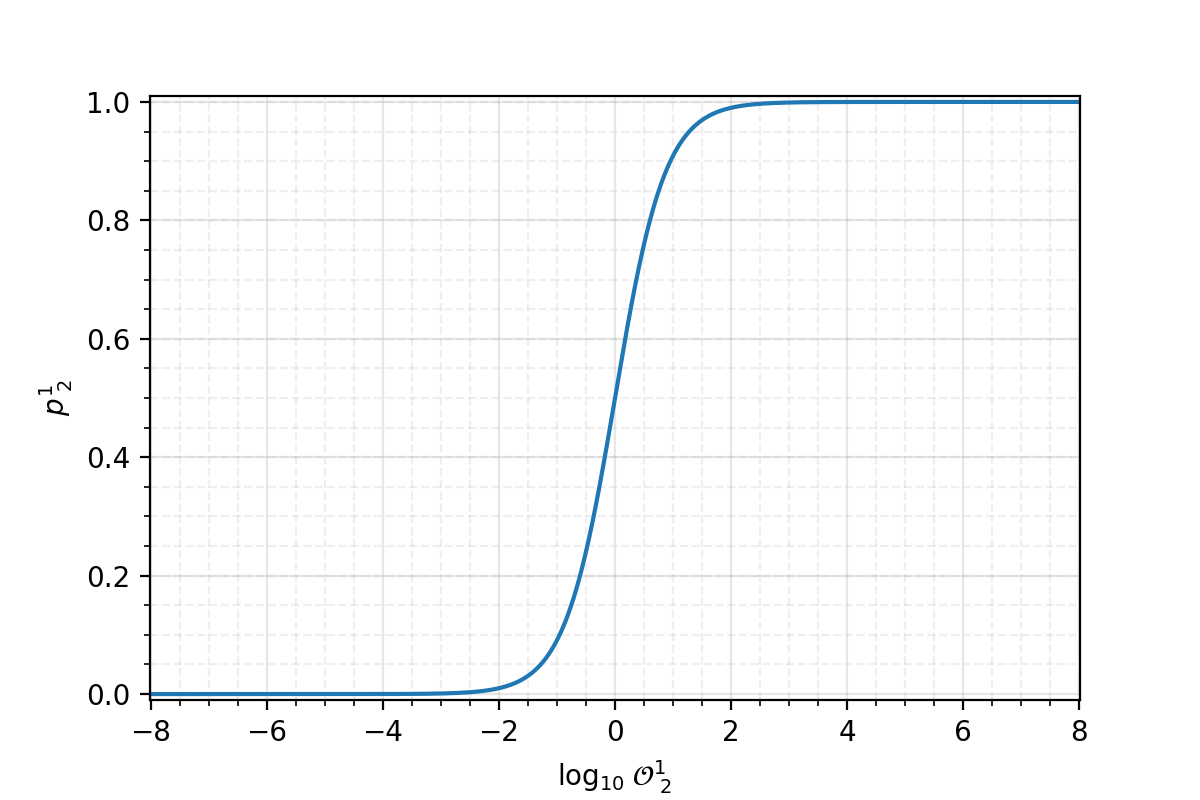
\includegraphics[width=\textwidth]{/figs/chapter5/log10odds_probability.png}
  \caption{The probability of hypothesis 1 being favored over hypothesis 2 when considering the $\mathrm{log}_{10} \; \mathcal{O}$. When $\mathrm{log}_{10} \; \mathcal{O} = 0$, the probability for each hypothesis is $50\%$. At odds ratios close to 100 (0.01) the evidence becomes heavily stacked towards one hypothesis or another.}
  \label{fig:log10odds_v_probability}
\end{figure}
Furthermore, we can map this probability to a ranking statistic that is more familiar to Frequentists. That is the one-tailed z-score which states the integrated probability density from $-\infty$ to a particular multiple of the standard deviation of a Gaussian function. A z-score of $0 \sigma$ indicates a $50\%$ probability, while a z-score of $5 \sigma$ is $\sim$ $1-10^-7$ probability. We place a plot of this below for convenience.
\begin{figure}
  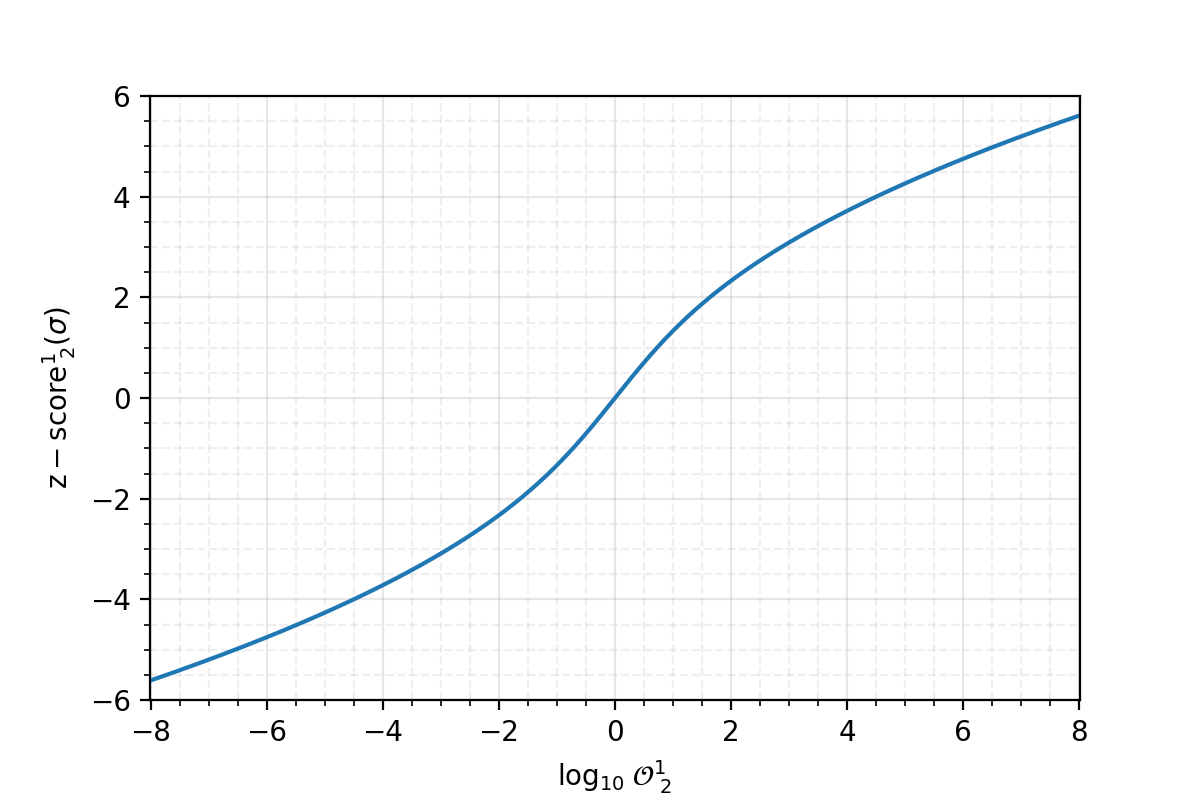
\includegraphics[width=\textwidth]{/figs/chapter5/log10odds_z_score.png}
  \caption{The Frequentist z-score pertaining to the same level of probability for  hypothesis 1 being favored over hypothesis 2 when considering the $\mathrm{log}_{10} \; \mathcal{O}$. When $\mathrm{log}_{10} \; \mathcal{O} = 0$, the z-score is $0 \sigma$ and the probability for each hypothesis is $50\%$. A z-score of $>5 \sigma$ has the same probability value as an odds ratio of $> 10^7$.}
  \label{fig:log10odds_v_z_score}
\end{figure}

One convenient property of odds ratios is that we can stack evidence from multiple events if we continue to measure new data with our same prior hypotheses. In this manner, it is possible to take low significant results from multiple experiments and gradually build evidence for a hypothesis over many experiments. This requires that each experiment is a statistically independent event from the others, which is for all intents and purposes guaranteed in gravitational wave astronomy.

\subsection{Bayesian Model Averaging}

Bayesian statistics is based centrally around inferences from Bayes theorem. And as such there is no distinction necessary for inferences over parameters and inferences over models themselves. This provides a simple way to extend a singular analysis into an ongoing inference over multiple data sets or over multiple hypotheses. It provides a robust method for comparing and combining multiple inferences when data are informative or uninformative. As such we describe a methodology for combining the results of multiple hypothesis inferences called Bayesian model averaging as found in Kass and Raftery.

The concept of Bayesian model averaging is to average over many different models after evaluating the marginal likelihood for each model. In particular, one considers a fiducial standard model, $A$, of which the marginal likelihoood of $A$ will be compared to every other model. Thus for $N$ models we generate $N$ Bayes factors, where model $A$'s Bayes factor is simply unity since it is the fiducial standard model. In the case that all of the Bayes factors, $B_i$, are not definitive for one model or another, we must consider the possibility that since our parameters are conditioned on the model that we have elected, that we must seriously consider the effect of choice of model on various parameters. Given a sufficiently large set of models we can try to extract knowledge about the parameters that describe our data by marginalizing over many models. The formalism for this procedure follows immediately from Bayes theorem. Consider the following marginal posterior probability distribution for some model:
\begin{equation}
    \mathcal{P}(H_i|D) = \frac{\mathcal{B}^{H_i\;\;}_{\;\;H_A} \; \pi(H_i)}{\sum_{i=1}^N \mathcal{B}^{H_i\;\;}_{\;\;H_A} \; \pi(H_i)}.
\end{equation}
Here we have the posterior probability of some hypothesis given the data ... and the prior probability that we had for each model $H_i$...
Next, we consider a parameter $x$ that is present in all models thus considered such that our marginal posterior probability on $x$ given all of the models can become:
\begin{equation}
    \mathcal{P}(x|D) = \sum_{i=1}^N \mathcal{P}(x| D, H_i) \; \mathcal{P}(H_i|D).
\end{equation}
Here $\mathcal{P}(x| D, H_i)$ represents the marginal posterior probability distribution of $x$ under a particular hypothesis $H_i$, and so we coherently combine our inferences from multiple models by marginalizing over models. While, in practice there are an infinite number of models from which to draw inference on, there are usually only a finite set of probable models that we desire to investigate. All other models we can set our prior probabilities $\pi(H_i)$ to $0$, or sufficiently close to $0$ that they do not contribute to the analysis.

In the face of model uncertainty with respect to a particular data set, this provides us a consistent method for combining the results of multiple models in a self-consistent manner.

\subsection{Multiple Data Sets: Combining Evidence}

\section{Derivation of the Thermodynamic Integration and Steppingstone methods}\label{sec:ti_ss_method_derivation}
\subsection{The Thermodynamic Integration Method}
From the Sec.~\ref{sec:methods} we learned about power-posteriors in Eq.~(\ref{eq:power_posterior}) and the thermodynamic integral given in Eq.~(\ref{eq:thermoint}). We follow resources \citep{annis2019thermodynamic} for the derivation and discussion here. Here we derive the thermodynamic integral by considering the following expression implied by the 2nd Fundamental theorem of Calculus:
\begin{equation}\label{eqn:ti_identity}
    \mathrm{ln} \, \mathcal{Z}_{\beta=1}\left(\mathbf{d}\right) - \mathrm{ln} \, \mathcal{Z}_{\beta=0}\left(\mathbf{d}\right) = \int^1_0 \left(\frac{d\left(\mathrm{ln} \, \mathcal{Z}_\beta \left(\mathbf{d}\right) \right)}{d\beta}\right) \, d\beta = \int^1_0 \frac{1}{\mathcal{Z}_\beta \left(\mathbf{d}\right)} \frac{d \, \mathcal{Z}_\beta \left(\mathbf{d}\right)}{d\beta} d\beta.
\end{equation}
For a properly normalized prior, $\pi(\vec{\theta}$, $\mathrm{ln} \, \mathcal{Z}_{\beta=0} \left(\mathbf{d}\right) = 0$. This leaves the marginal likelihood at $\beta=1$ that we are interested in, the untempered $\mathrm{ln} \, \mathcal{Z} \left(\mathbf{d}\right)$. Now we can expand Eq.~\ref{eqn:ti_identity} as:
\begin{equation}
    \mathrm{ln} \, \mathcal{Z} \left(\mathbf{d}\right) = \int_0^1 \frac{\int \frac{d}{d\beta} \left[\pi\left(\vec{\theta}\right) \, \mathcal{L} \left(\mathbf{d}|\vec{\theta} \right)^\beta \right]\, d\vec{\theta} d\vec{\theta}}{\int \pi\left(\vec{\theta}\right) \, \mathcal{L}\left(\mathbf{d}|\vec{\theta} \right)^\beta \, d\vec{\theta}}.
\end{equation}
Suppressing parenthetical arguments on $\theta$ and $\mathbf{d}$ for clarity we can arrive at the following expression by taking the derivative in the numerator we then arrive at:
\begin{equation}
    \mathrm{ln} \, \mathcal{Z} = \int^1_0 \frac{\int \pi \, \, \, \left(\mathrm{ln} \, \mathcal{L}\right) \, \, \, \mathcal{L}^{\beta} d\theta}{\int \pi \mathcal{L}^{\beta} d\theta} d\beta.
\end{equation}
Using Bayes theorem we can replace the numerator and denominator with $\mathcal{P}_\beta = \pi \mathcal{L}^\beta / \mathcal{Z}_\beta$ to get:
\begin{equation}
    \mathrm{ln} \, \mathcal{Z} = \int^1_0 \frac{\int \mathcal{P}_\beta \, \left(\mathrm{ln} \, \mathcal{L}\right) d\theta}{\int \mathcal{P}_\beta   d\theta} d\beta = \int^1_0 \langle \mathrm{ln} \, \mathcal{L} \rangle_{\mathcal{P}_\beta} \, d\beta,.
\end{equation}
Thus, the logarithm of the untempered evidence is given by the one dimensional integral in Eq.~(\ref{eq:thermoint}).
where $\langle \mathrm{ln} \, \mathcal{L} \rangle_{\mathcal{P}_\beta}$ represents the average untempered log-likelihood under the measure described by the power-posterior distribution at $\beta$. Said in another way, this is the average untempered log-likelihood when drawing samples from the power-posterior distribution at $\beta$. We suppress this notation to write $\langle \mathrm{ln} \, \mathcal{L} \rangle_{\mathcal{P}_\beta} \equiv \langle \mathrm{ln} \, \mathcal{L} \rangle_\beta$ in the main-body of the text. Thus simulating from power-posterior distributions with $\beta$ between $0$ and $1$ provide a means to estimating the logarithm of the untempered evidence for the model and thus present a tractable way towards Bayesian model selection and comparison. This method is an ubiased estimator of the evidence provided that samples of $\langle \mathrm{ln} \, \mathcal{L} \rangle_\beta$ can be drawn in an unbiased manner from power-posteriors~\citep{carlson2016partition}.

It is convenient to describe additional derivatives of the thermodynamic integrand as they will be useful as references in the next section. In general, $\mathrm{n}^{\mathrm{th}}$ derivatives of the form $\mathrm{ln} \, \mathcal{Z}$ can be solved as~\citep{gradshteyn2015table}\footnote{Note that the solution in~\cite{gradshteyn2015table} has a minor typo, which we correct here.}:
\begin{equation}\label{eqn:gradshteyn_derivatives}
    \frac{d^n}{d\beta^n}\left( \mathrm{ln} \, \mathcal{Z} \right) = \sum_{k=1}^{n} \frac{(-1)^{(k+1)} {{n}\choose{k}}}{k \mathcal{Z}^k} \frac{d^n}{d\beta^n} \left(\mathcal{Z}^k\right).
\end{equation}
The first derivative, $n=1$, we have already solved as being $\langle \mathrm{ln} \, \mathcal{L} \rangle_\beta$. The next derivative, $n=2$, was found in~\cite{friel2014improving} as $\mathrm{Var}(\mathrm{ln} \, \mathcal{L})_\beta$, which is the variance of the untempered log likelihood samples when drawn from the power-posterior at $\beta$. We solve the next derivative, $n=3$, as:
\begin{equation}\label{eqn:third_ti_deriv}
    \frac{d^3}{d\beta^3}\left( \mathrm{ln} \, \mathcal{Z}\right) = \langle \left(\mathrm{ln} \, \mathcal{L} \right)^3\rangle_\beta + 2 \langle \mathrm{ln} \, \mathcal{L} \rangle^3_\beta - 3 \langle \left(\mathrm{ln} \, \mathcal{L} \right)^2\rangle_\beta \langle \mathrm{ln} \, \mathcal{L}\rangle_\beta.
\end{equation}
An astute observation would be to recognize that the pattern here follows that the $\mathrm{n}^{\mathrm{th}}$ derivative of $\mathrm{ln} \, \mathcal{Z}$ follow the pattern of the $\mathrm{n}^{\mathrm{th}}$ cumulants of the power-posterior distribution at $\beta$~\cite{friel2014improving, carlson2016partition}. The term $\mathcal{Z}$ describes a partition function for the posterior distribution $\mathcal{P}$~\citep{carlson2016partition, lamont2019correspondence}, and $\mathrm{ln} \, \mathcal{Z}$ can be thought of as a cumulant generating function~\citep{kardar2007statistical}. This relationship can make computation of values of high order derivatives more numerically stable since cumulants of order $\ge 2$ are shift-invariant~\cite{kardar2007statistical}. We can make the transformation of variables, $\widetilde{\mathrm{ln} \, \mathcal{L}} \equiv \mathrm{ln} \, \mathcal{L} - \mathrm{ln} \, \mathcal{L}_{\mathrm{max}}$ for every power-posterior before calculating Eq.~(\ref{eqn:third_ti_deriv}). We have tested this on high-order derivatives and found it to be both accurate and numerically stable, although we have found that the parallel-tempered \emph{emcee} sampler~\citep{emcee,vousden:2016} may not be stable enough to permit high-order derivatives to be accurate in all cases.

The thermodynamic integrand with the next two derivatives are shown in Fig.~\ref{fig:gooseneck_linear} for the permissive $\delta \phi$ prior choice ($\mathrm{log}_{10} A \in U[-10, -5.5], \, n \in U[-1, 3), \, f_0 \in U[10, 100]~Hz$) with a linear in $\beta$ scale. We also produce this plot in the logarithmic scale in~\ref{fig:gooseneck_log} where inspection of the curvature of the thermodynamic integrand is easier to see. These plots are helpful to inspect for places where the integrand may not be well sampled in $\beta$ and hence require additional inverse-temperatures~\cite{liu2016evaluating, de2011free, de2013comparison}. Of particular note is the instability in the second (third) subplot of Fig.~\ref{fig:gooseneck_log} where the second (third) derivative is not smooth in $\beta$. Even in the first subplot, where we expect the thermodynamic integrand to be smooth and monotonically increasing as $\beta$ goes from $0$ to $1$, there is some numerical instability at $\beta \sim 10^{-9}$. This implies, perhaps, the need for a better tempering sampler or bias-corrective terms in the sampling such as those found in~\cite{oates2017control,evans2019thermodynamic}. The instability is so slight however that we do not expect it to significantly impact the Bayes factor estimation, but it is a potential source of error in the numerical integration.

\begin{figure}[th]
\centering
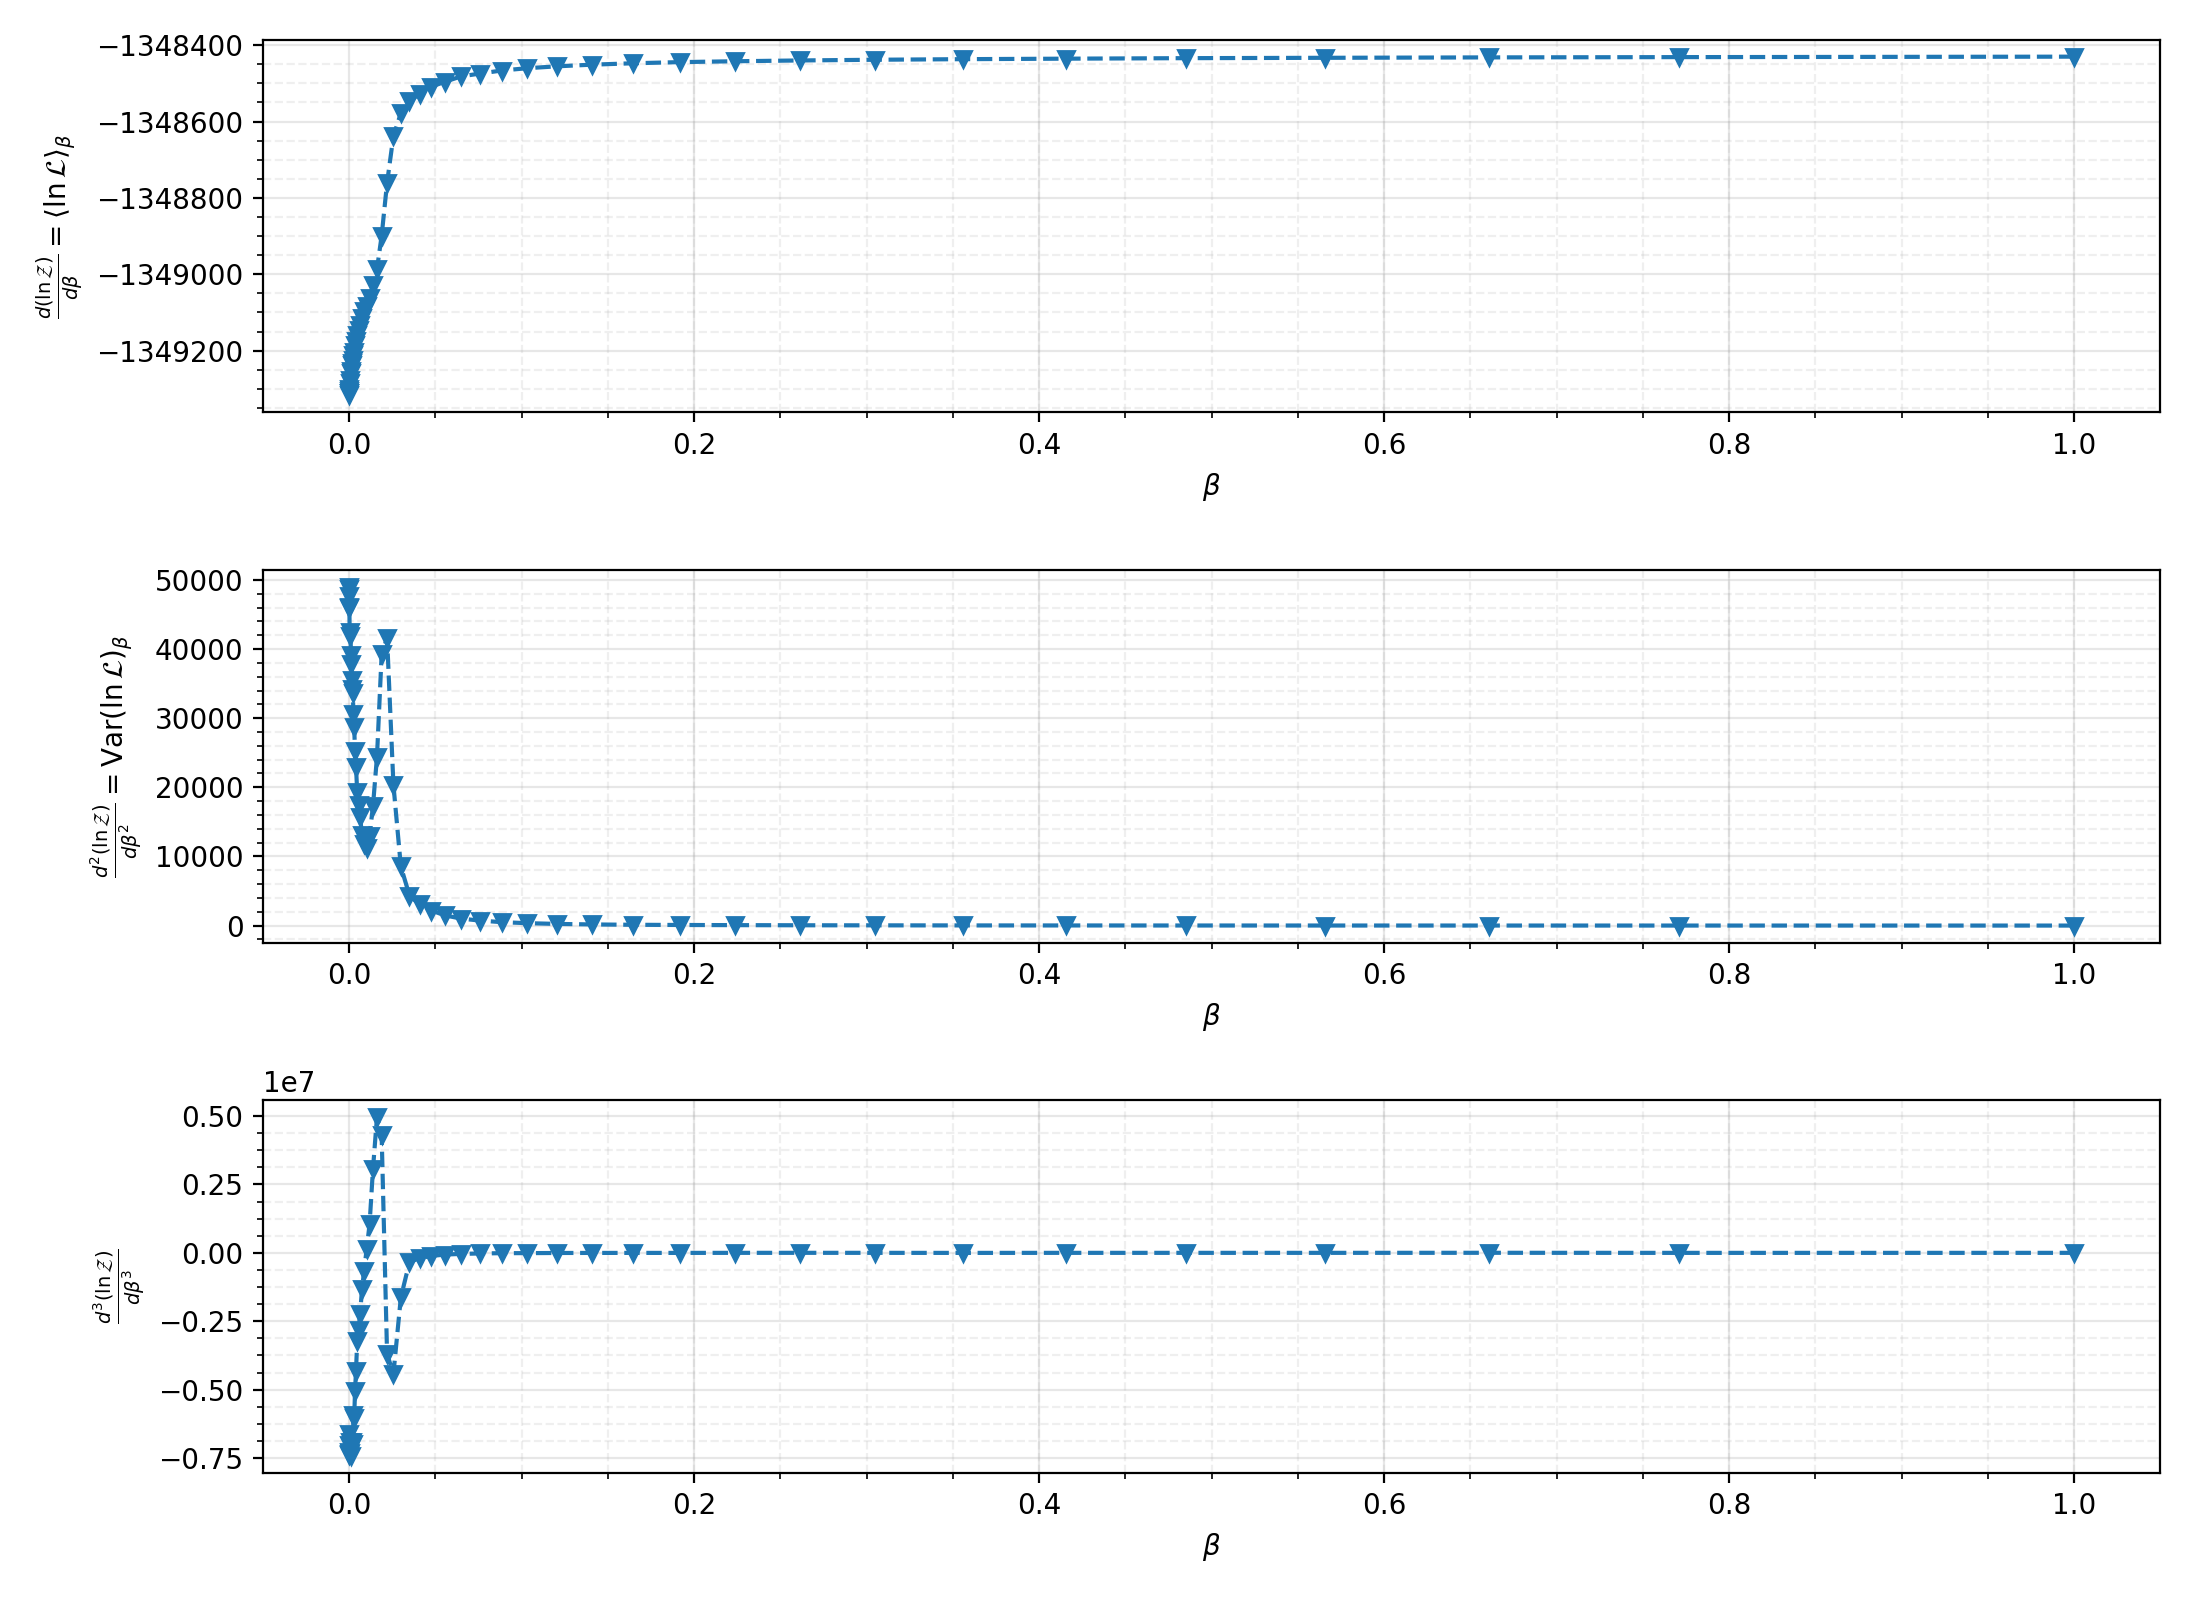
\includegraphics[width=0.9\columnwidth]{figs/chapter6/gooseneck_plots_linear.png}
\caption{The subplots of the thermodynamic integrand and subsequent derivatives of the thermodynamic integral. (\textit{Top}) The thermodynamic integrand when compared to the inverse-temperature $\beta$. The curve should be smooth and montonic, however it is very difficult to inspect the integrand on a linear $\beta$ scale. (\textit{Middle}) The second derivative of the logarithm of the evidence is the variance of the power-posterior at an inverse temperature $\beta$. There is some indication that an inflection point happens in the curvature of the integrand at high temperature. (\textit{Bottom}) The third derivative of the logarithm of the evidence is also the third-order cumulant of the power-posterior distributions at an inverse-temperature $\beta$. It is difficult to inspect the behavior of this derivative on the linear $\beta$ scale.}
\label{fig:gooseneck_linear}
\end{figure}

\begin{figure}[th]
\centering
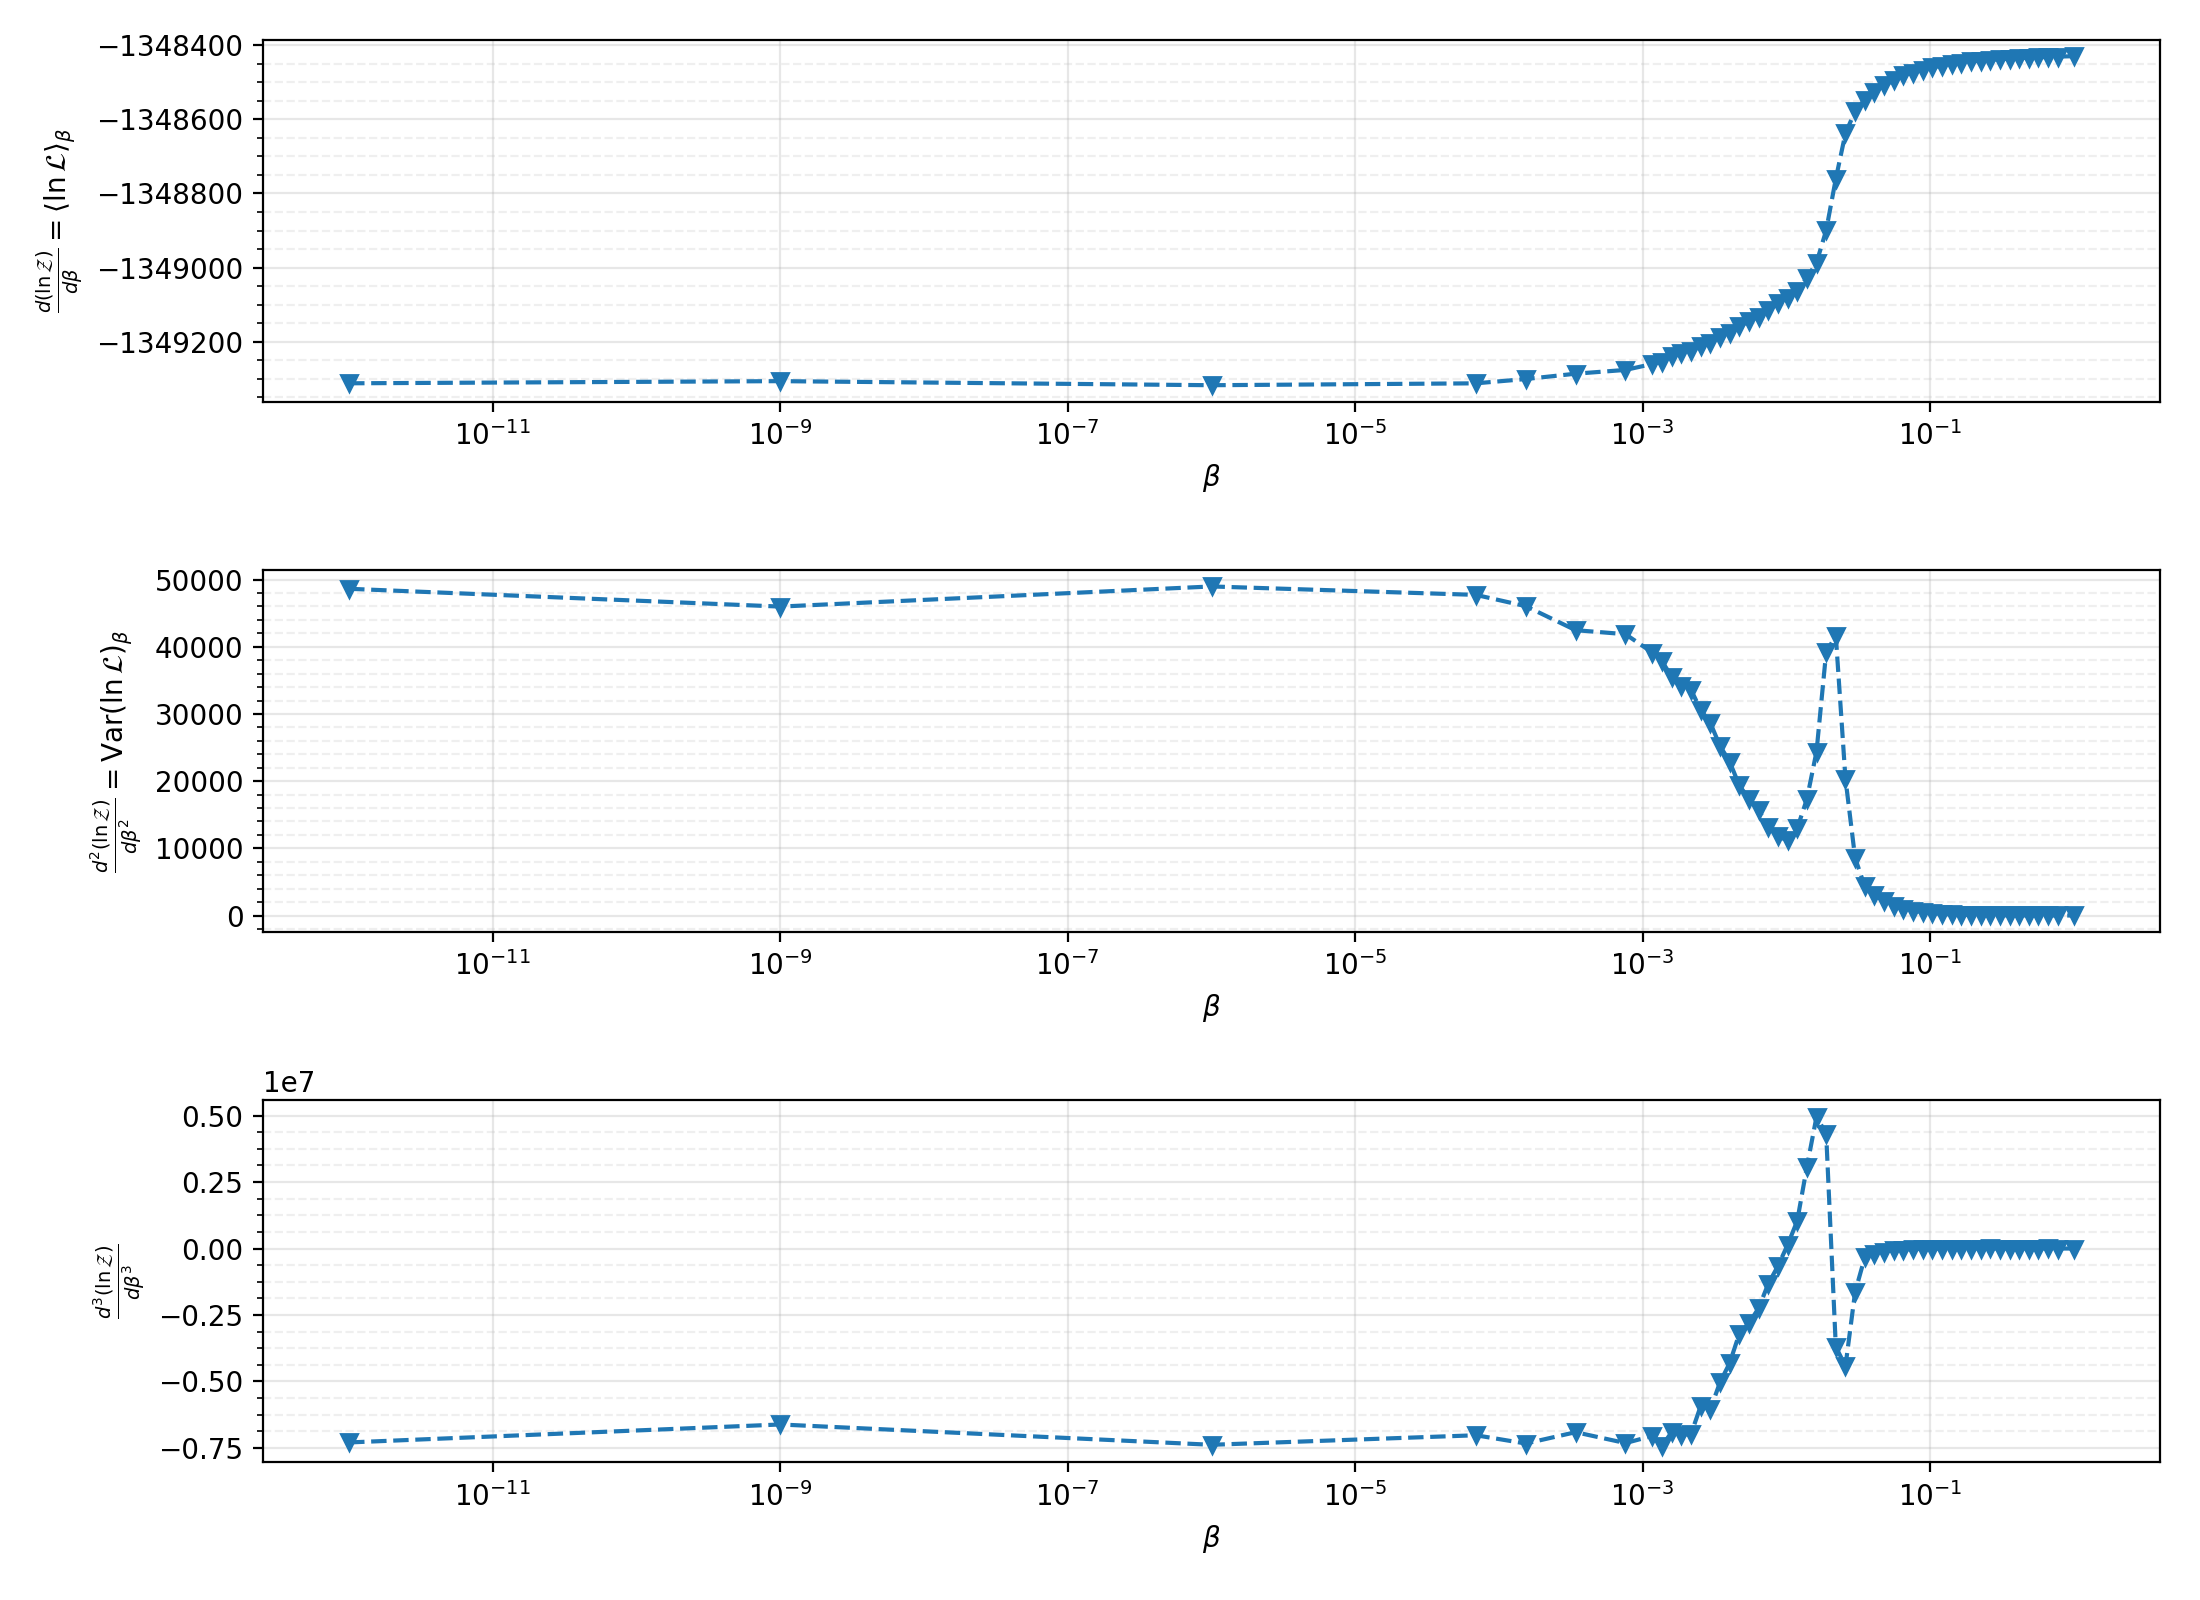
\includegraphics[width=0.9\columnwidth]{figs/chapter6/gooseneck_plots_log.png}
\caption{The subplots of the thermodynamic integrand and subsequent derivatives of the thermodynamic integral. (\textit{Top}) The thermodynamic integrand when compared to the inverse-temperature $\beta$. The curve should be smooth and montonic, however there is some indication at $\beta = 10^{-9}$ that this condition is not strictly met in the Markov Chain Monte Carlo simulation. (\textit{Middle}) The second derivative of the logarithm of the evidence is the variance of the power-posterior at an inverse temperature $\beta$. This function should also be smooth however there is some indication that at high temperature that the derivatives are not stable. (\textit{Bottom}) The third derivative of the logarithm of the evidence is also the third-order cumulant of the power-posterior distributions at an inverse-temperature $\beta$. Here we can see that the derivatives are not very sable or smooth. This may motivate moving our analysis to new multi-tempered samplers that are optimized for thermodynamic integration.}
\label{fig:gooseneck_log}
\end{figure}

\subsubsection{Numerical Quadrature}
The thermodynamic integral in Eq.~(\ref{eq:thermoint}) can be estimated through numerical quadrature rules such as the trapezoidal rule, or Simpson's rule. Because $\beta$ for thermodynamic integration are typically not uniformly distributed between $0$ and $1$, it is beneficial to consider integration rules that do not depend on equally spaced abscissa. A polynomial interpolant that does not make use of derivatives of the function or equally spaced abscissa is the Newton's divided difference interpolant, see~\cite{brun1953generalization, selmer1958numerical, abramowitz1965handbook} for examples of how to construct these polynomials. Other  interpolants, and thus integration rules, can be constructed, see ~\cite{abramowitz1965handbook} for examples.

The simplest rule that we consider here is the trapezoidal rule which can be written for thermodynamic integration as:
\begin{equation}
    \widehat{\mathrm{ln} \, \mathcal{Z}}_{\mathrm{Trapz}} = \sum_{i=0}^{N_\beta-1} \frac{1}{2} \left(\beta_{i+1} - \beta_i \right) \left(\langle \mathrm{ln} \, \mathcal{L} \rangle_{\beta_{i+1}} + \langle \mathrm{ln} \, \mathcal{L} \rangle_{\beta_{i}} \right)
\end{equation}
Here $N_\beta$ represents the number of $\beta$ being summed over in the integration estimation. The error corrective term to the trapezoidal rule can be found by integrating the next-to-leading order Taylor polynomial correction~\citep{abramowitz1965handbook}, yielding:
\begin{equation}
    \widehat{\mathrm{ln} \, \mathcal{Z}}_{\mathrm{Trapz \, +}} \approx \widehat{\mathrm{ln} \, \mathcal{Z}}_{\mathrm{Trapz}} + \sum_{i=0}^{N_\beta-1} -\frac{1}{12} \left(\beta_{i+1} - \beta_i \right)^2 \left(f'(\beta_{i+1}) - f'(\beta_{i}) \right).
\end{equation}
Here $f'(\beta_i)$ represents the second derivative of $\mathrm{ln} \, \mathcal{Z}$ with respect to $\beta$. It was found in~\cite{friel2014improving} that this corresponds to the variance of the untempered log likelihood as drawn from the power-posterior at $\beta_i$.

Simpson's rule for unequally spaced abscissa under Newton's divided difference interpolation~\citep{easa1988area} is:
\begin{equation}
    \widehat{\mathrm{ln} \, \mathcal{Z}}_{\mathrm{Simps}} = \sum_{\mathrm{i\, is\, even}, \. i=0}^{N_\beta-2} \frac{h_i + h_{i+1}}{6} \left [ A \, \langle \mathrm{ln} \, \mathcal{L} \rangle_{\beta_{i}} + B \, \langle \mathrm{ln} \, \mathcal{L} \rangle_{\beta_{i+1}} + C \, \langle \mathrm{ln} \, \mathcal{L} \rangle_{\beta_{i+2}}\right ],
\end{equation}
for the expressions:
\begin{equation}
\begin{array}{lll}
     A &= \frac{(2h_i - h_{i+1})}{h_i} \\ \\ 
     B &= \frac{(h_i+h_{i+1})^2}{h_i h_{i+1}} \\ \\
     C &= \frac{(2h_{i+1} - h_i)}{h_{i+1}}. \\ \\
\end{array}
\end{equation}
Here  $h_i \equiv \beta_{i+1} - \beta_i$, and $h_{i+1} \equiv \beta_{i+2} - \beta_{i+1}$. The error corrective term for Simpson's rule can thus be solved in the same manner as for the trapezoidal rule and we find:
\begin{equation}
    \widehat{\mathrm{ln} \, \mathcal{Z}}_{\mathrm{Simps \, +}} \approx \widehat{\mathrm{ln} \, \mathcal{Z}}_{\mathrm{Simps}} + \sum_{\mathrm{i\, is\, even}, \, i=0}^{N_\beta-2} \frac{1}{72}\left(\beta_{i+2} - \beta_{i} \right)^2 (\beta_i - 2\beta_{i+1} + \beta_{i+2})\frac{f''(\beta_{i+2}) - f''(\beta_i)}{\beta_{i+2} - \beta_i}.
\end{equation}
Here $f''(\beta_i)$ represents the third derivative of $\mathrm{ln} \, \mathcal{Z}$ with respect to $\beta$, which is in Eq.~\ref{eqn:third_ti_deriv}.

The cubic integration rule for unequally spaced abscissa under Newton's divided difference interpolation can be found in~\cite{brun1953generalization,selmer1958numerical,chambers1989estimating} or can be derived through the tools in~\cite{abramowitz1965handbook}. We also use the cubic integration rule, and in particular we use the form given in~\cite{chambers1989estimating}:
\begin{equation}
    \widehat{\mathrm{ln} \, \mathcal{Z}}_{\mathrm{cubic}} = \sum_{\mathrm{i\, is\, a \, multiple \, of \, 3}, \, i=0}^{N_\beta-3} \frac{h_i + h_{i+1} + h_{i+2}}{12} \left [A \, \langle \mathrm{ln} \, \mathcal{L} \rangle_{\beta_{i}} + B \, \langle \mathrm{ln} \, \mathcal{L} \rangle_{\beta_{i+1}} + C \, \langle \mathrm{ln} \, \mathcal{L} \rangle_{\beta_{i+2}} + D \, \langle \mathrm{ln} \, \mathcal{L} \rangle_{\beta_{i+3}}\right ],
\end{equation}
for expressions:
\begin{equation}
\begin{array}{llll}
     A &= \frac{3h_i^2 -h_{i+1}^2 +h_{i+2}^2 +2 h_i h_{i+1} - 2h_i h_{i+2}}{h_i (h_i + h_{i+1})} \\ \\
     B &= \frac{(h_i + h_{i+1} + h_{i+2})^2 (h_i + h_{i+1} - h_{i+2})}{h_{i} h_{i+1} (h_{i+1} h_{i+2})} \\ \\
     C &= \frac{(h_i + h_{i+1} + h_{i+2})^2 (h_{i+1} + h_{i+2} - h_i)}{h_{i+1} h_{i+2} (h_i + h_{i+1})} \\ \\
     D &= \frac{h_i^2 - h_{i+1}^2 +3 h_{i+2}^2 - 2h_i h_{i+2} + 2 h_{i+1} h_{i+2}}{h_{i+2}(h_{i+1} + h_{i+2})}.\\ \\
\end{array}
\end{equation}
Here we have defined $h_i \equiv \beta_{i+1} - \beta_{i}$, $h_{i+1} \equiv \beta_{i+2} - \beta_{i+1}$, and $h_{i+2} \equiv \beta_{i+3} - \beta_{i+2}$.

We exercise caution in describing the thermodynamic integral through a higher order polynomial quadrature rule as it may not be well described by polynomials. Thus there may be very little incentive for going to higher order polynomial rules as improved accuracy is not always guaranteed by going to higher order polynomial integration rules~\citep{epperson1987runge}. It is important to note that we treat the logarithm of the evidence as an unknown quantity which we are trying to infer the value of, and so we must treat the evidence as a random variable. Without prior information we should exercise caution when trusting one of these quadrature rules above the others. Our inference is more confident when these quadrature rules agree on the numerical value of the logarithm of the evidence.

Future studies may make use of Taylor series polynomials for unequally spaced abscissa, ratios of Taylor series polynomials through the Pad$\textrm{\'e}$ approximant for improved accuracy~\citep{press1992pade}, or other interpolant functions. Improvement in numerical integration for thermodynamic integration may also be improved by focusing on increasing the number of inverse-temperatures $\beta$ and/or by improved placement of $\beta$.

\subsubsection{Monte Carlo Error}
Here we follow the discussion from \cite{annis2019thermodynamic} who provide a heuristic for estimating the Monte Carlo error to estimating the thermodynamic integral as first given in \cite{friel2008marginal}. A variance of the thermodynamic integral estimator, $\widehat{\mathrm{ln} \, \mathcal{Z}}$, from Monte Carlo error can be found in two steps. First, calculate the thermodynamic integral for each sample of untempered log likelihoods drawn from the power-posterior at $\beta$. For $N$ samples drawn from each power-posterior this generates $N$ thermodynamic integral values. The integration should be done relative to the numerical quadrature technique that one is trying to estimate the Monte-Carlo error for. This represents the sample variance of the thermodynamic integration. The variance of the mean value of the logarithm of the evidence can be calculated via:
\begin{equation}
    \sigma^2_{\mathrm{MC}} = \frac{1}{N} \sigma^2_{\mathrm{sample}}.
\end{equation}
Here, $\sigma^2_{\mathrm{MC}}$ represents the Monte-Carlo variance for the thermodynamic integration estimator while $\sigma^2_{\mathrm{sample}}$ is the sample variance and $N$ represents the number of available samples. See Fig.~\ref{fig:ti_monte_carlo_error} for a visualization of this procedure.

\begin{figure}[th]
\centering
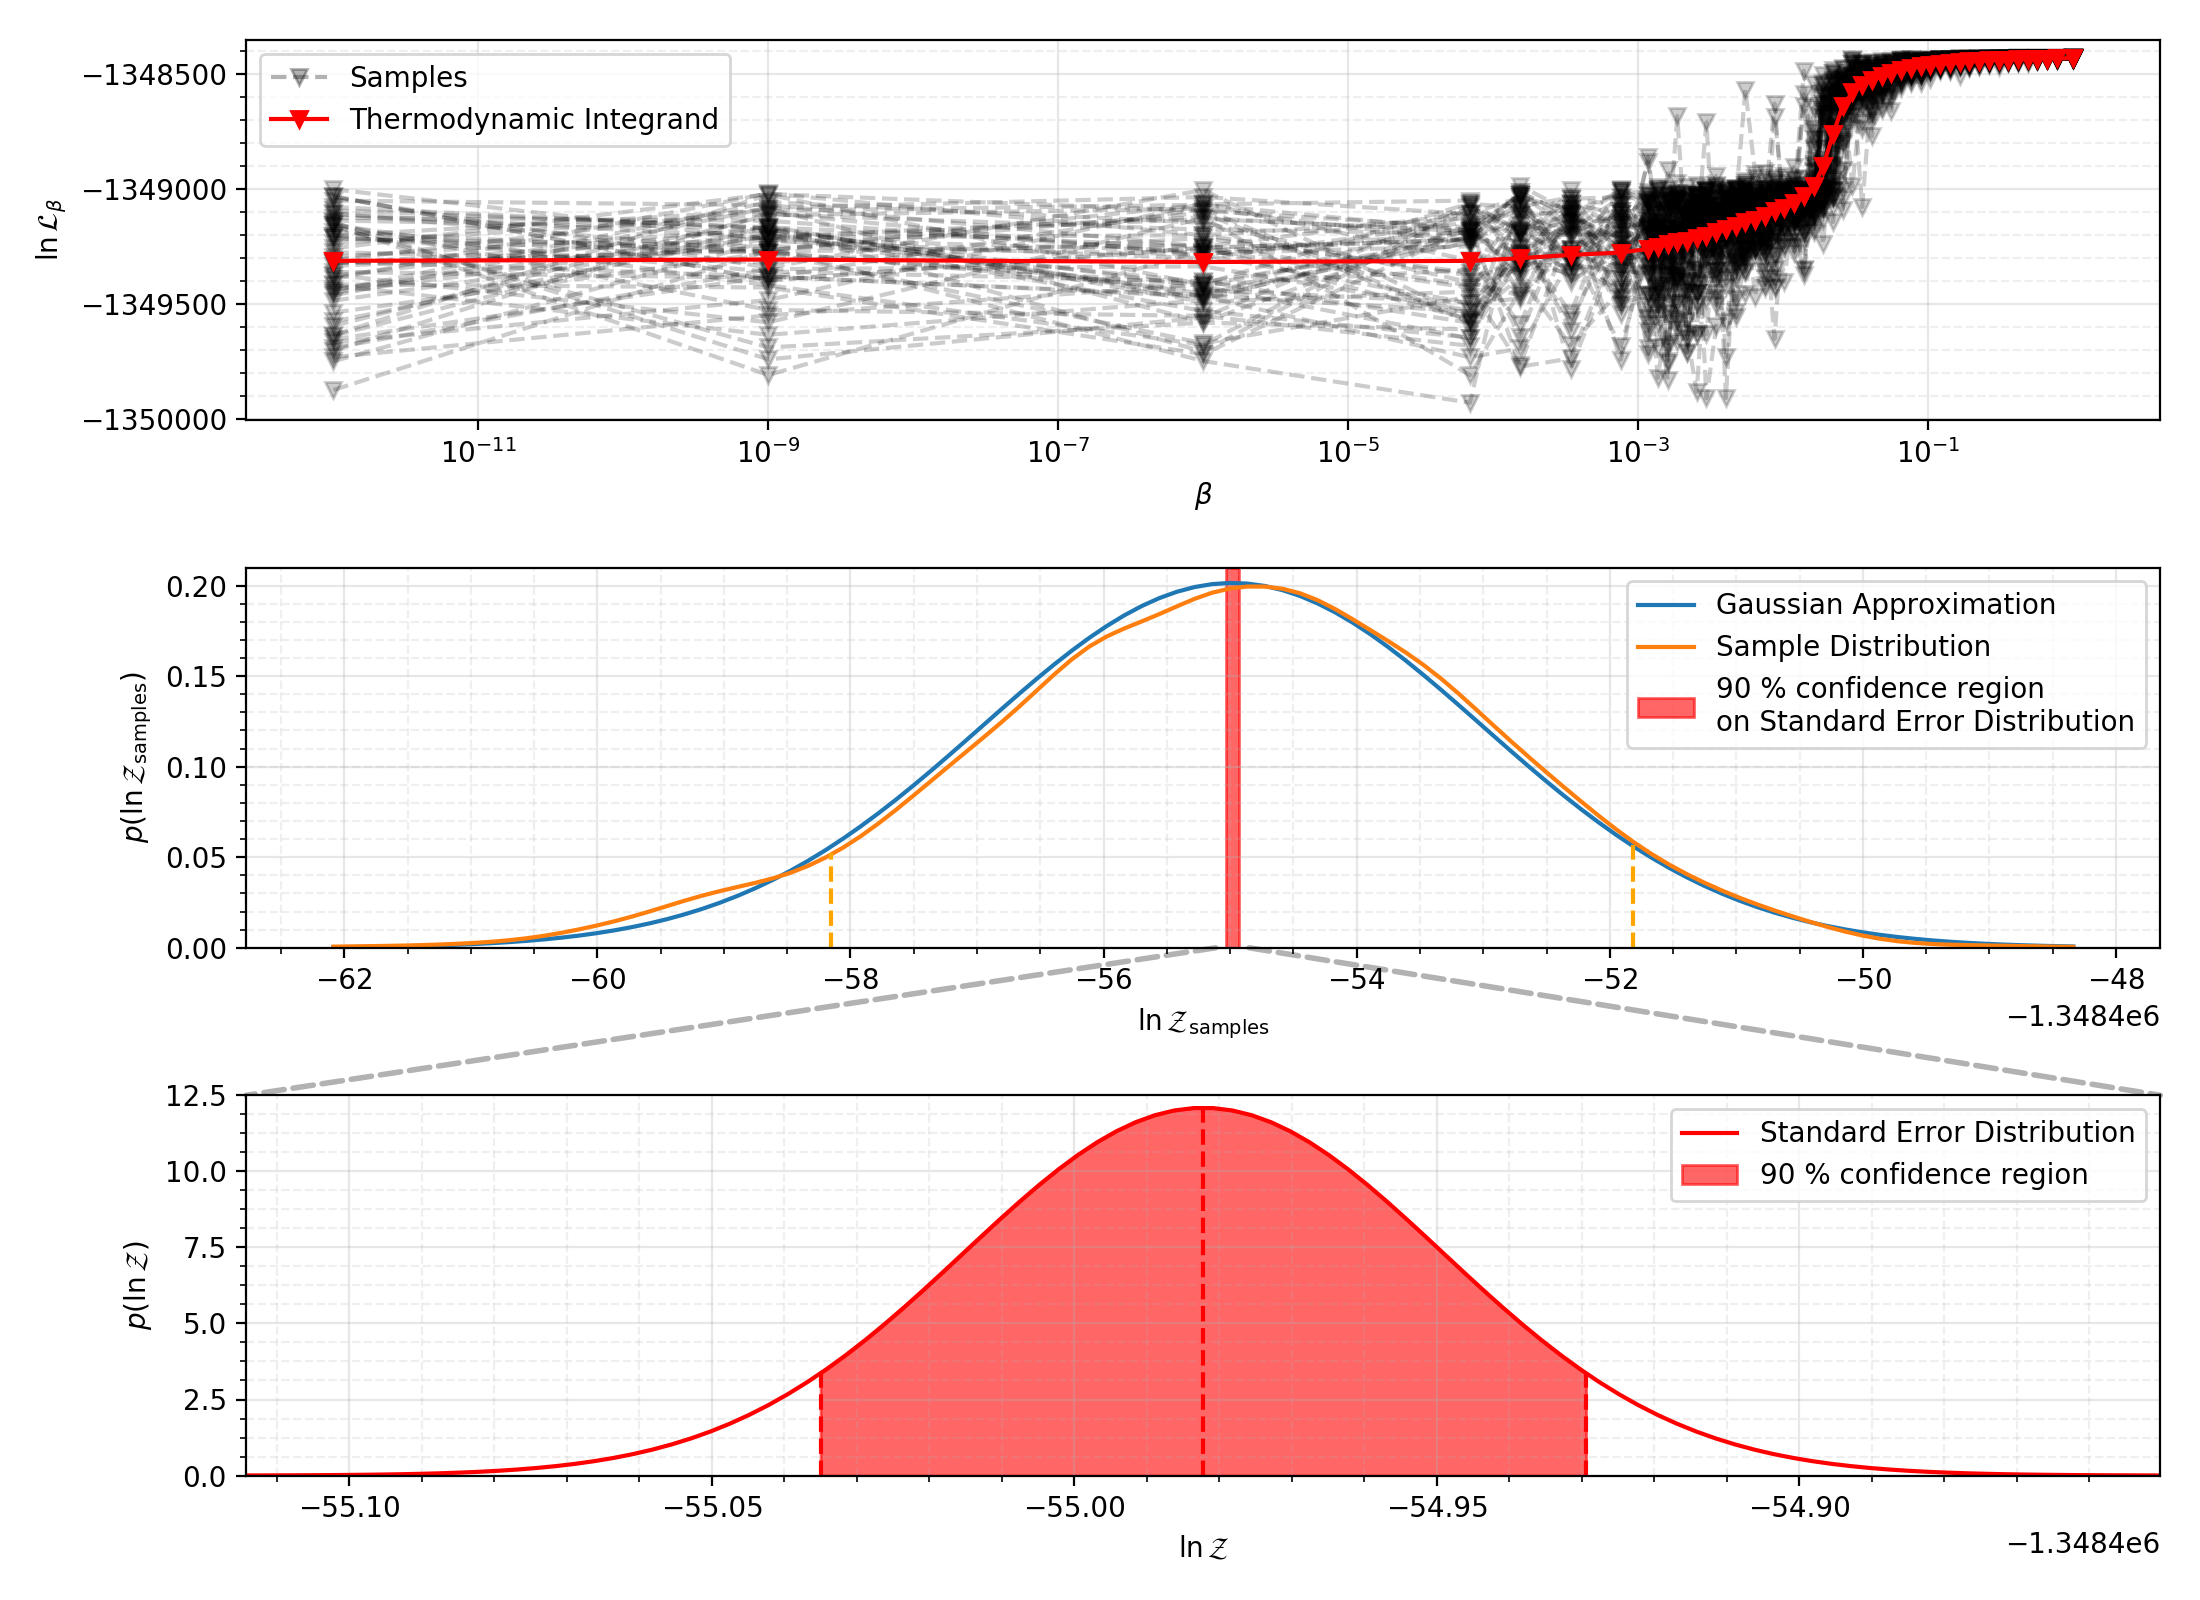
\includegraphics[width=0.9\columnwidth]{figs/chapter6/ti_monte_carlo_error.png}
\caption{The first subplot denotes the untempered log-likelihood samples when drawn from the power-posteriors at $\beta$. The expectation value of the untempered log-likelihood when drawn from these power-posteriors is the thermodynamic integrand and is plotted in red. The thermodynamic integral over all geometric paths given from the samples is drawn in the second subplot. The sample-log-integral distribution is approximately a Gaussian distribution. The standard error of the mean value of the log evidence is given by the sample standard deviation divided by the square root of the number of samples. The $90 \%$ confidence interval on the sample distribution in the log-evidence is drawn in dashed orange lines. The $90\%$ confidence region from this standard error is shaded in red. The final subplot is a zoom-in on this $90 \%$ confidence region showing the error estimate on the thermodynamic integral due to Monte Carlo sampling. This, when combined with the convergence error, is used in the final error estimate on the log-evidence of the thermodynamic integral.}
\label{fig:ti_monte_carlo_error}
\end{figure}

Repeated runs where the random seed for the Markov-Chain Monte Carlo analysis was changed has shown that the variance estimate from presented in~\cite{annis2019thermodynamic} is a plausible confidence interval estimate for Monte Carlo error. It has also shown good agreement with the steppingstone Monte Carlo error estimate which uses the same samples as those in thermodynamic integration.

\subsubsection{Convergence Error}
The procedure of estimating the marginal likelihood from power-posterior simulation requires that the power-posteriors all converge to the proper distribution. To first order, this requires inspection of the thermodynamic integrand over the course of the MCMC analysis. To next order, this would require that sequential cumulants of the power-posterior also stabilizes. In the limit that the MCMC analysis has converged all of the power-posterior distributions will be stationary as a function of MCMC iteration. During the course of the study we did not fully investigate the stationarity of the full power-posterior distribution through inspection of all of the cumulants, but rather focused on the stationarity of the thermodynamic integrand across each temperature. This resulted in investigating the stationarity of the the thermodynamic integral as well.

An accurate depiction of the power-posterior distribution for a particular temperature requires that all of the samples be independent and identically distributed samples (this is sometimes called \textif{i.i.d.} in the statistics literature)~\cite{annis2019thermodynamic}. Gathering independent and identically distributed samples can be done by calculating the autocorrelation length of the MCMC chains from a particular temperature. In practice, PyCBC Inference calculates the autocorrelation length of all of the temperature chains and uses the largest autocorrelation length as the autocorrelation length for all temperatures. This is a safe and conservative practice for ensuring that samples drawn from the MCMC simulation are not correlated. Thus, to track the thermodynamic integrand at various iterations in the MCMC simulation we divide the MCMC analysis into $12$ equally spaced partitions  based on the number of MCMC iterations that the analysis has undergone. In practice any number of partitions will do, but it is computationally intensive to sample more partitions. The partitions do not need to be equally spaced in MCMC iterations but we find equally spaced partitions to be useful for visualization of the progression of the thermodynamic integrand. Using this number of partitions, each partition is segmented in half, where the first half is discarded as burn-in samples, and the autocorrelation length is calculated from the remaining samples. Then independent samples are drawn from this segment spaced out by autocorrelation length. This is the generic procedure of the $\mathrm{n_{acl}}$ algorithm implemented in PyCBC for drawing independent samples from the Markov chains. The partitioning is shown in Fig.~\ref{fig:nacl_segments}. Having drawn independent samples from $12$ segments of the MCMC analysis we can visually inspect the stability of the thermodynamic integrand at $12$ iterations in the MCMC analysis. We can also inspect the convergence of the thermodynamic integral. When the logarithm of the evidence has converged to $\mathcal{O}(10^{-2}$ accuracy, we usually consider the power-posteriors to have converged to their final distribution. We base our inference on convergence on the worst quadrature method, the trapezoidal rule for thermodynamic integration, as a means to be conservative. Higher order quadrature rules can converge more rapidly than the trapezoidal rule, however, the more closely aligned the numerical quadrature estimates the more confidence we can attain in the accuracy of the thermodynamic integration. Figure~\ref{fig:integrand_convergence} shows the progression of the convergence of the thermodynamic integrand as a function of the MCMC iteration. Figure~\ref{fig:integral_convergence} shows the convergence rate of the thermodynamic integral as a function of the MCMC iteration for a variety of integration techniques.

\begin{figure}[th]
\centering
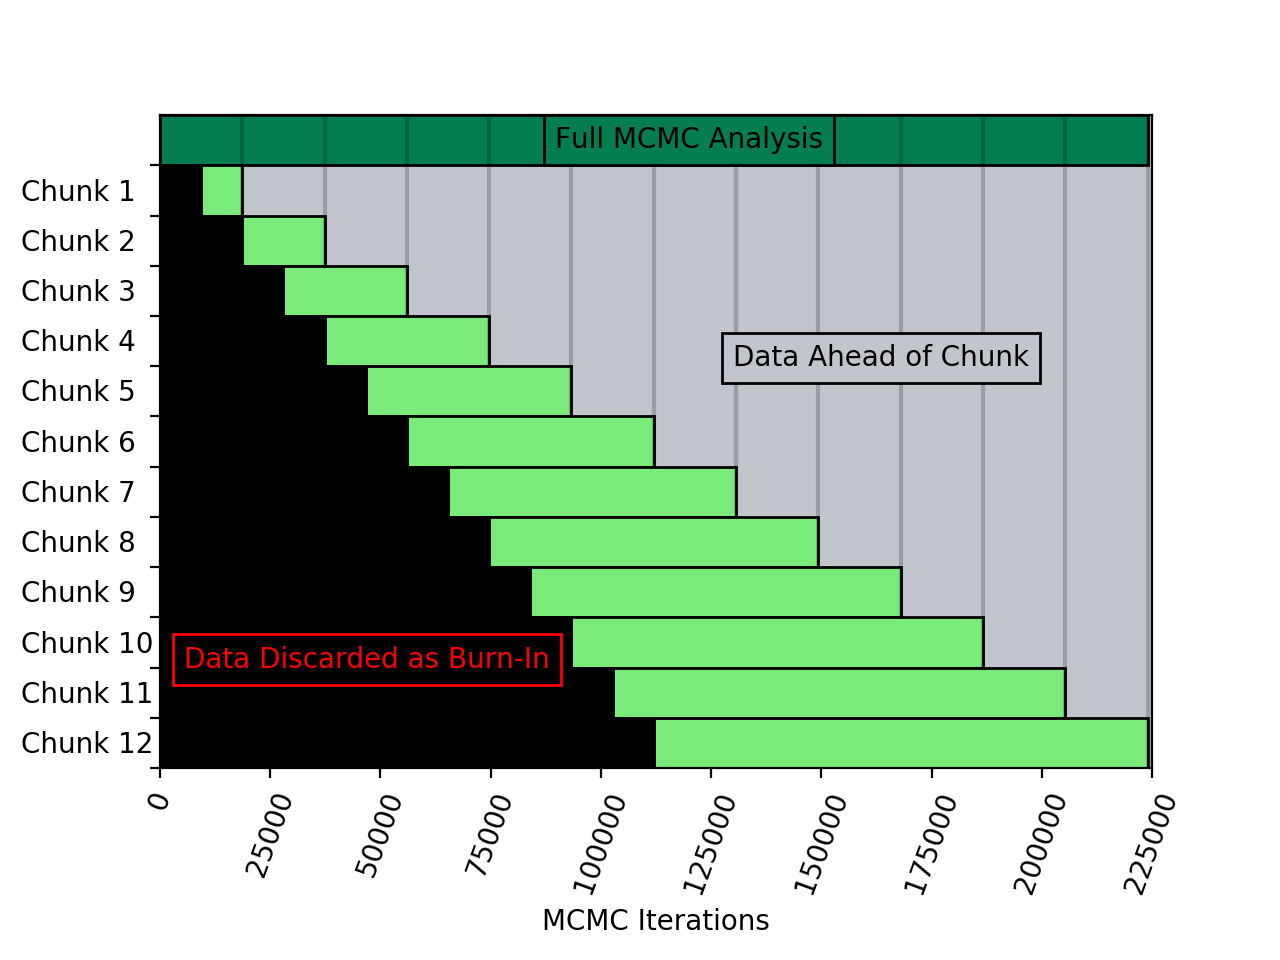
\includegraphics[width=0.9\columnwidth]{figs/chapter6/convergence_segmentation_lvc_sim.png}
\caption{The partitioning of the MCMC analysis to check on the convergence of the thermodynamic integrand and the thermodynamic integration. The dark-green bar at the top represents all of the samples collected by the MCMC analysis. This segment is divided into 12 segments represented by the light gray lines. The light-green segments represent chunks that independent samples can be drawn from. The dark region represents samples discarded as burn-in samples for the MCMC. The dark grey region represents data that is ahead of the chunk and thus not used in drawing independent samples for that chunk. Chunk $12$ produces the identical samples as drawing independent samples according to the $\mathrm{n_{acl}}$ algorithm from PyCBC at the end of the analysis.}
\label{fig:nacl_segments}
\end{figure}

\begin{figure}[th]
\centering
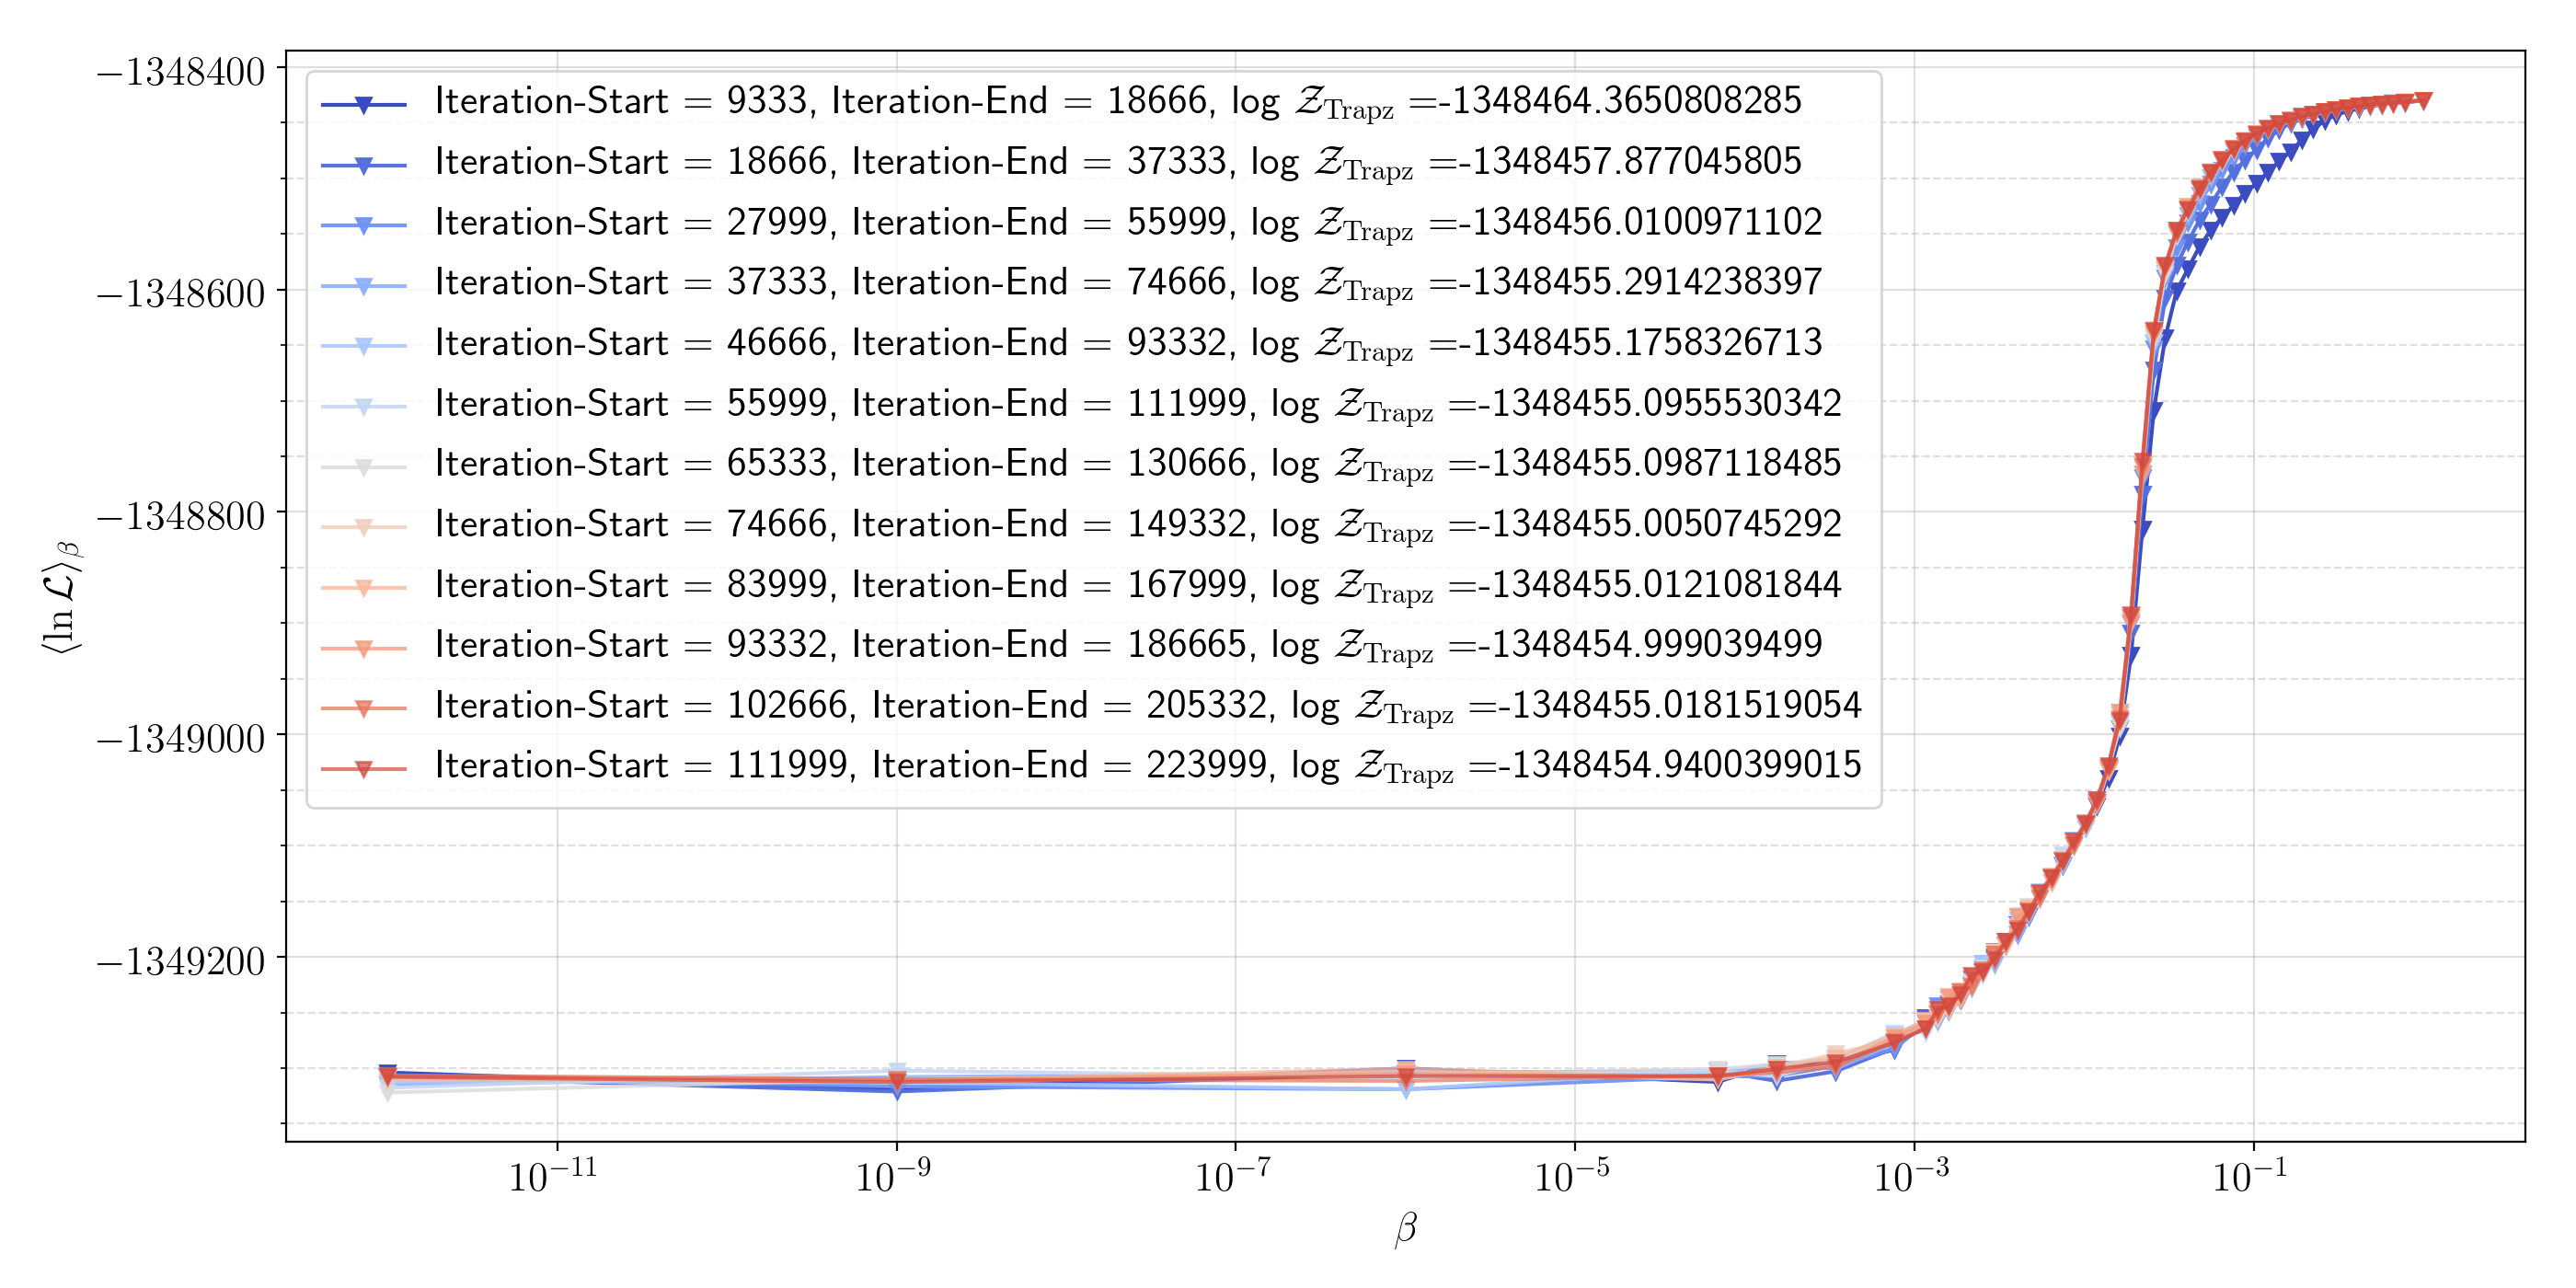
\includegraphics[width=0.9\columnwidth]{figs/chapter6/lsc_sim_integrand_progress.png}
\caption{The convergence of the thermodynamic integrand for the unconstrained $\delta \phi$ prior choice on the $p$-$g$ mode instability model. The Iteration-Start denotes the point is taken from a segment beginning with that MCMC iteration and ending with the MCMC iteration denoted as Iteration-End. These iterations correspond to the segments found in Fig.~\ref{fig:nacl_segments}. The logarithm of the evidence is shown also in the figure caption, and it can be noted that as the MCMC analysis progresses the integral converges to a set value. The thermodynamic integrand can be visually seen to converge to the S-like curve seen in the figure. Early in the analysis the curve can be mishaped as the power-posteriors have not all converged. Experience has told us tha the power-posteriors that take the longest to converge tend to be in the region where the average log likelihood changes rapidly. Here this is in the region between $\beta$ $\in$ ($10^{-2} - 1$).}
\label{fig:integrand_convergence}
\end{figure}

\begin{figure}[th]
\centering
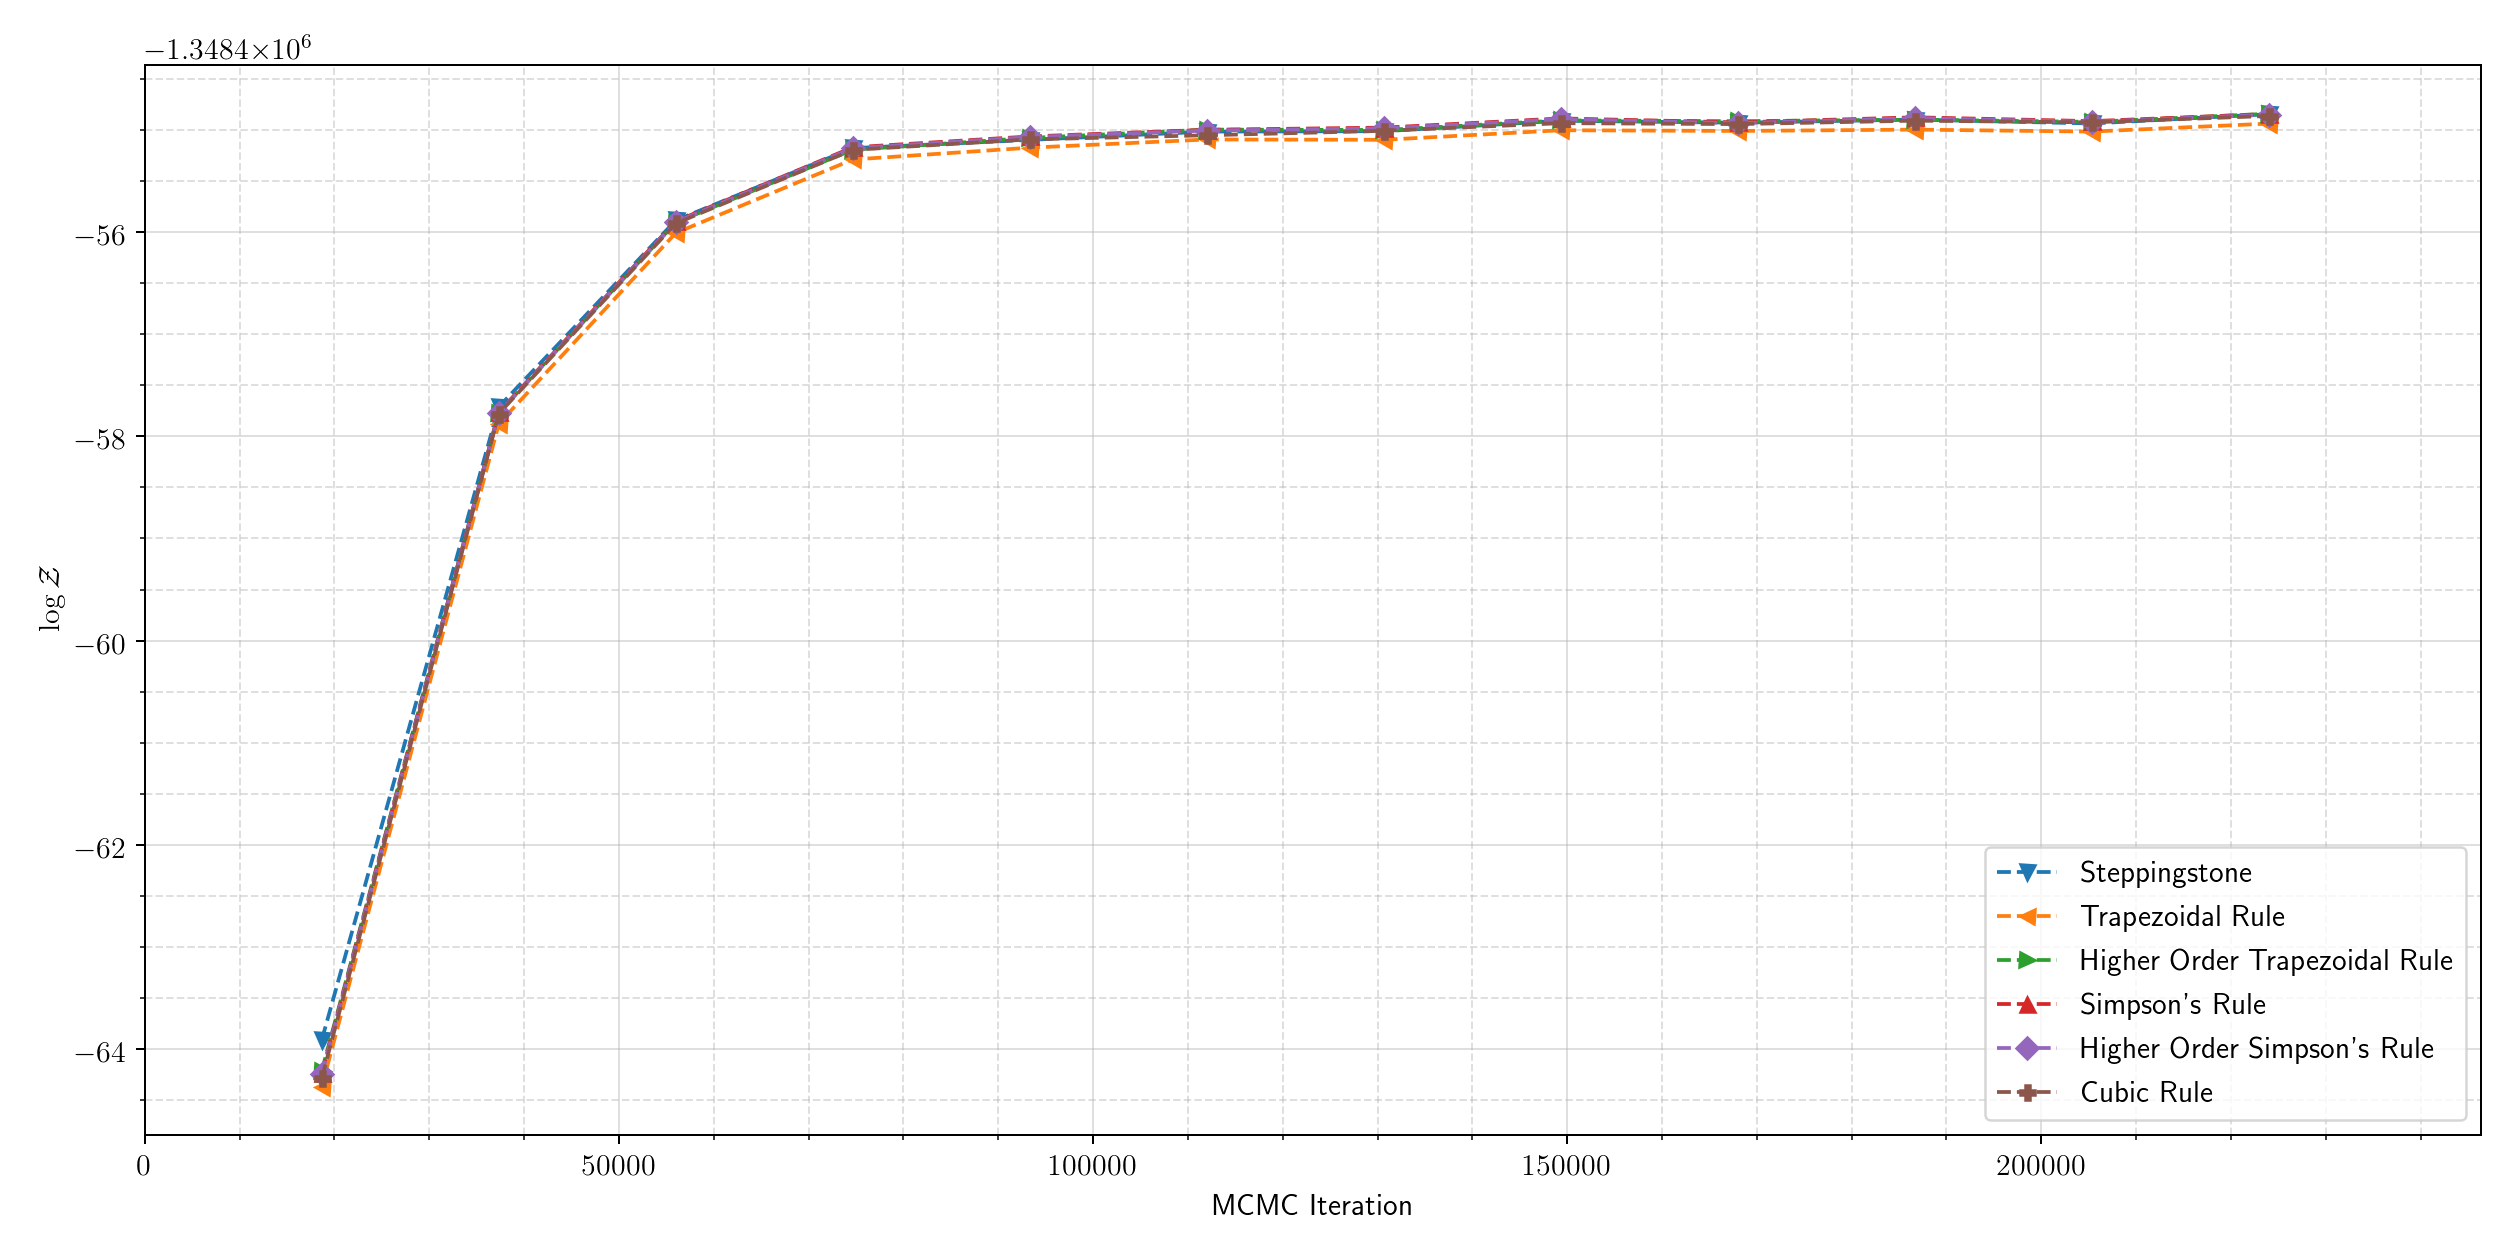
\includegraphics[width=0.9\columnwidth]{figs/chapter6/lvc_sim_evidence_convergence.png}
\caption{The convergence of the thermodynamic integral for the unconstrained $\delta \phi$ prior choice on the $p$-$g$ mode instability model as a function of the MCMC iteration. These choice of points of iterations correspond to the segments found in Fig.~\ref{fig:nacl_segments}. As the analysis progresses the logarithm of the evidence from all methods tend towards a fixed value.}
\label{fig:integral_convergence}
\end{figure}

The absolute value of the difference between the last two thermodynamic integration estimates from this partitioning are then used as the standard deviation of the error for the log evidence due to convergence error, $\sigma_{\mathrm{convergence}}$:
\begin{equation}
    \sigma_{\mathrm{convergence}} \sim  \, \mid \mathrm{ln} \, \mathcal{Z}_{\mathrm{partition \,} N} - \mathrm{ln} \, \mathcal{Z}_{\mathrm{partition \,} N-1} \mid
\end{equation}
This provides a rough estimate for ensuring that we do not terminate the MCMC analysis too early and thus give ourselves overconfidence about the true value of logarithm of the evidence. Previous analyses such as those in \cite{de2018tidal} did not make use of this technique and the analysis is terminated based on the number of independent samples collected in the posterior distribution. This is an insufficient metric for inference analyses based on Bayesian model selection through multi-tempered MCMC simulation. We use this estimate for $\sigma_{\mathrm{convergence}}$ in Eq.~\ref{eq:errorprop}.

During the development of this technique a similar technique based on a moving-block bootstrap method was developed in~\cite{Russel:2018pqv} for error analysis of the logarithm of the evidence from the thermodynamic integration method. We have not investigated this technique thoroughly to compare its performance with our own method.

\subsubsection{Temperature Placement Bias}
The placement of inverse-temperatures $\beta$ affects the results of the numerical integration for the evidence\citep{lartillot2006computing, xie2010improving}. This study has a particular bias at the low-end of $\beta \to 0$ because it does not include $\beta = 0$ in the numerical integration. This tail-end bias at small $\beta$ is much, much lower than the resolution of the Monte Carlo error and the convergence error and so it is irrelevant to the final results. However, future practice should always include $\beta =0$.

Research into the proper placement of $\beta$ is ongoing in the field of Statistics~\citep{annis2019thermodynamic}. We followed the suggestions in~\cite{liu2016evaluating} on placing temperatures where the thermodynamic integrand changed rapidly. With $51$ inverse-temperatures it is incredibly unlikely that the main results of the Bayes factors being $\sim 0.7$ are biased by discretization error outside of the statistical uncertainties. This is implied by the agreement of the results between thermodynamic integration, the steppingstone, and the Savage-Dickey density ratio methods. In Fig.~\ref{fig:lvc_sim_log_evidence_distr} there is some slight disagreement on the exact value of the marginal log likelihood, but it seems to cancel out in the Bayes factor since all models share the same temperature ladder (see Fig~\ref{fig:lvc_sim_uni_ceos_bayes_distr}).

One method for improving the temperature ladder would be to use the method of~\cite{friel2014improving} by using the intersection of the slopes of the thermodynamic integrand from two adjacent power-posteriors as a new position for additional temperatures. We could go further by using the intersections of higher-order polynomials using the expressions for the derivatives of the thermodynamic integrand. However, this is not likely to be fruitful in this study as our error at the moment appears dominated by Monte Carlo error and convergence error. Future studies using multi-tempering techniques may make use of this method in refining temperature placement.

It is our opinion that the placement of inverse-temperatures, if it cannot be solved analytically, should be considered a question of inference. That is to say, given a prior belief on an appropriate distribution on the placement of inverse-temperatures, how should one adjust the placement of inverse-temperatures given the results of the numerical quadrature routine? Bayesian quadrature is a promising area of research meant to address optimal placement of abscissa for numerical integration. It is likely that the thermodynamic integration method would likely greatly benefit from this sort of an approach. See~\cite{diaconis1988bayesian} for an initial formulation and~\cite{briol2015probabilistic} for a modern perspective, especially with respect to thermodynamic integration.

\subsection{The Steppingstone Method}
The steppingstone method is very similar in many respects to thermodynamic integration in that it requires multiple inverse-temperatures between $0$ and $1$ to calculate. The motivation for steppingstone is that it uses importance sampling between adjacent temperatures to estimate the contribution to the marginal likelihood $\mathcal{Z}$ at each interval $\beta_{i-1}$-$\beta_i$. Before we derive the steppingstone method we provide a brief, but useful derivation of another often used identity, called the harmonic mean estimator for the evidence. For the following section we suppress use of $\vec{\theta}$ and $\mathbf{d}$.

For the derivation of the harmonic mean estimator we follow a simplified version of the derivation presented in \citep{newton1994approximate}. From the definition of the marginal likelihood we can write:
\begin{equation}
    \frac{1}{\mathcal{Z}} = \frac{1}{\int \pi \, \mathcal{L} \, d\theta}.
\end{equation}
Since we only deal with proper priors we can substitute the numerator with $\int \pi d\theta = 1$. This gives:
\begin{equation}
    \frac{1}{\mathcal{Z}} = \frac{\int \pi \, d\theta}{\int \pi \, \mathcal{L} \, d\theta}.
\end{equation}
Now we multiply both the numerator and denominator by $\mathcal{P}/\mathcal{P}$ to get:
\begin{equation}
    \frac{1}{\mathcal{Z}} = \frac{\int \frac{\pi}{\mathcal{P}} \mathcal{P} \, d\theta}{\int \frac{\pi \, \mathcal{L}}{\mathcal{P}}\mathcal{P} \, d\theta}.
\end{equation}
Which we simplify using Bayes theorem to substitute out for $1/\mathcal{P}$ to give:
\begin{equation}
    \frac{1}{\mathcal{Z}} = \frac{\int \frac{\pi \mathcal{Z}}{\pi \mathcal{L}} \mathcal{P} \, d\theta}{\int \frac{\pi \, \mathcal{L} \mathcal{Z}}{\pi \mathcal{L}}\mathcal{P} \, d\theta}.
\end{equation}
Cancelling out terms of $\pi$ and moving terms of $\mathcal{Z}$ out of the integral to cancel, this gives:
\begin{equation}\label{eqn:HME}
    \frac{1}{\mathcal{Z}} = \frac{\int \frac{1}{\mathcal{L}} \mathcal{P} \, d\theta}{\int \mathcal{P} \, d\theta} = \int \frac{1}{\mathcal{L}} \mathcal{P} \, d\theta.
\end{equation}
Therefore we can express the inverse of the evidence as:
\begin{equation}
    \frac{1}{\mathcal{Z}} = \langle \mathcal{L}^{-1} \rangle_{\mathcal{P}},
\end{equation}
which is to say that the inverse of the evidence is given as the average value of the inverse of the likelihood when sampled from the measure defined by the posterior distribution. This is the harmonic mean estimator of the evidence, and although it is correct in theory, it typically misbehaves numerically and computationally. It is also worth noting as~\cite{xie2010improving} points out that the harmonic mean estimator is not sensitive to the prior distribution which runs contradictory to the heart of Bayesian model comparison. We will use this identity in the derivation of the steppingstone estimator.

We follow~\cite{annis2019thermodynamic} in the derivation of the steppingstone estimator. Recall from Eq. \ref{eq:thermoint} that the marginal likelihood can be expressed as:
\begin{equation}
    \mathrm{ln} \, \mathcal{Z} = \mathrm{ln} \, \mathcal{Z}_{\beta=1} - \mathrm{ln} \, \mathcal{Z}_{\beta=0},
\end{equation}
which is equivalent to:
\begin{equation}
    \mathcal{Z} = \frac{\mathcal{Z}_{\beta=1}}{\mathcal{Z}_{\beta=0}}.
\end{equation}
For, say, a hundred equally spaced temperatures between $0$ and $1$ this motivates the following re-expression:
\begin{equation}
    \mathcal{Z} = \frac{\mathcal{Z}_{\beta = 0.01}} {\mathcal{Z}_{\beta = 0}}  
    \times \frac{\mathcal{Z}_{\beta = 0.02}} {\mathcal{Z}_{\beta = 0.01}}
    \times \ldots \times \frac{\mathcal{Z}_{\beta = 0.99}} {\mathcal{Z}_{\beta = 0.98}} \times \frac{\mathcal{Z}_{\beta = 1}} {\mathcal{Z}_{\beta = 0.99}}.
\end{equation}
The general form for this is:
\begin{equation}\label{eqn:ssa_prod_series}
     \mathcal{Z} = \prod_{i=1}^{N_\beta} \frac{\mathcal{Z}_{\beta_{i}}}{\mathcal{Z}_{\beta_{i-1}}}.
\end{equation}
Here we use the ordering on $\beta$, as $\beta_0=0 < \beta_1 < ... < \beta_{N_\beta -1} < \beta_{N_\beta} = 1$. Finally, then, consider the evidence for the  power-posterior at inverse-temperature $\beta_i$ given as:
\begin{equation}
    \mathcal{Z}_{\beta_i} = \int \pi \mathcal{L}^{\beta_i} \, d\theta.
\end{equation}
We now divide by $1$ via $\int \pi \, d\theta$ and multiply by $1$ via $\mathcal{P}_{\beta_{i-1}} \, / \, \mathcal{P}_{\beta_{i-1}}$ in the numerator and denominator to get:
\begin{equation}
    \mathcal{Z}_{\beta_i} = \left(\int \frac{\pi \mathcal{L}^{\beta_i}}{\mathcal{P}_{\beta_{i-1}}} \mathcal{P}_{\beta_{i-1}} \, d\theta \right )\bigg / \left( \int \frac{\pi}{\mathcal{P}_{\beta_{i-1}}} \mathcal{P}_{\beta_{i-1}} \, d\theta \right).
\end{equation}
Using Bayes theorem we substitute $\mathcal{P}_{\beta_{i-1}}$ = $(1/\mathcal{Z}_{\beta_{i-1}}) \, \pi \, \mathcal{L}^{\beta_{i-1}}$ to get:
\begin{equation}
    \mathcal{Z}_{\beta_i} = \left (\int \frac{\pi \mathcal{L}^{\beta_i} \mathcal{Z}_{\beta_{i-1}}}{\pi \mathcal{L}^{\beta_{i-1}}} \mathcal{P}_{\beta_{i-1}} \, d\theta \right) \bigg / \left(\int \frac{\pi \mathcal{Z}_{\beta_{i-1}}}{\pi \mathcal{L}^{\beta_{i-1}}} \mathcal{P}_{\beta_{i-1}} \, d\theta\right).
\end{equation}
Terms of $\mathcal{Z}_{\beta_{i-1}}$ are independent of $\theta$ and so can be moved out of the integral where they cancel, and we can cancel terms of $\pi$ to get:
\begin{equation}
    \mathcal{Z}_{\beta_i} = \left(\int \frac{ \mathcal{L}^{\beta_i} }{\mathcal{L}^{\beta_{i-1}}} \mathcal{P}_{\beta_{i-1}} \, d\theta\right) \bigg / \left(\int \frac{1}{ \mathcal{L}^{\beta_{i-1}}} \mathcal{P}_{\beta_{i-1}} \, d\theta\right).
\end{equation}
Finally we recognize that in the denominator we have Eq.~\ref{eqn:HME} for the inverse of the evidence at the inverse-temperature $\beta_{i-1}$, and in the top we can simplify terms so as to get:
\begin{equation}
    \mathcal{Z}_{\beta_i} = \mathcal{Z}_{\beta_{i-1}} \int \mathcal{L}^{\beta_i - \beta_{i-1}}  \mathcal{P}_{\beta_{i-1}} \, d\theta.
\end{equation}
Thus we arrive at the key ingredient for the steppingstone estimator:
\begin{equation}\label{eqn:ssa_identity}
    \frac{\mathcal{Z}_{\beta_i}}{\mathcal{Z}_{\beta_{i-1}}} = \int \mathcal{L}^{\beta_i - \beta_{i-1}}  \mathcal{P}_{\beta_{i-1}} \, d\theta = \langle \mathcal{L}^{\beta_i - \beta_{i-1}} \rangle_{\mathcal{P}_{\beta_{i-1}}}.
\end{equation}
This can be uncomfortably summarized as saying, in the interval of inverse-temperatures between $\beta_{i-1}$ and $\beta_i$, the ratio of the evidences between successive inverse-temperatures is given by the average of the likelihood raised to the difference in the inverse-temperatures when samples for the likelihood are drawn from the power-posterior distribution for the smaller of the  inverse-temperatures in the inverse-temperature interval. We suppress some of the notation in Eq.~(\ref{eqn:ssa_identity}) such that $\langle \mathcal{L}^{\beta_i - \beta_{i-1}} \rangle_{\mathcal{P}_{\beta_{i-1}}} \equiv \langle \mathcal{L}^{\beta_i - \beta_{i-1}} \rangle_{\beta_{i-1}}$ We finally combine Eq.~(\ref{eqn:ssa_identity}) into Eq.~(\ref{eqn:ssa_prod_series}) to achieve the steppingstone estimator for the evidence:
\begin{equation}\label{eqn:steppingstone}
    \mathcal{Z} = \prod_{i=1}^{N_\beta} \langle \mathcal{L}^{\beta_i - \beta_{i-1}} \rangle_{\beta_{i-1}}. 
\end{equation}
Some care needs to be taken in the implementation of Eq.~(\ref{eqn:steppingstone}) as the form presented is not numerically stable and we often must use the log likelihood and log evidence in place of the likelihood and the evidence. A numerically stable form of the logarithm of Eq.~(\ref{eqn:steppingstone}) is presented in~\cite{xie2010improving}. It is noted to exhibit some level of bias as an estimator of the marginal likelihood due to its logarithmic form. The bias is noted to be small, and it was shown in~\cite{xie2010improving} that the steppingstone estimator typically outperforms the trapezoidal rule for thermodynamic integration in terms of accuracy. This bias can be mitigated by increasing the number of temperatures and/or improving their placement between $0$ and $1$~\citep{xie2010improving}.

For the steppingstone estimator we can use the same samples as for the thermodynamic integration method. Optimal temperature placement for the steppingstone estimator is an active area of research~\citep{annis2019thermodynamic}.
\subsubsection{Monte Carlo Error}
In~\cite{xie2010improving} there is an expression for the estimated variance of the logarithmic steppingstone estimator using an approximation method called the $\delta$ method~\citep{oehlert1992note}. The expression in~\cite{xie2010improving} for the variance of the logarithm of the evidence is however not presented in a numerically stable version. We use a numerically stabilized version of the variance estimator in our study. We have found the variance estimate from the $\delta$ method is typically comparable to the thermodynamic integration method's Monte-Carlo error. Repeated runs where the random seed for the Markov-Chain Monte Carlo analysis was changed has shown that the variance estimate from presented in~\cite{xie2010improving} is a plausible confidence interval estimate for Monte Carlo error.  

\subsubsection{Convergence Error}
The method for calculating the error on the steppingstone estimator due to convergence error is algorithmically identical to the thermodynamic integration method.

\subsubsection{Temperature Placement Bias}
At the current time optimal placement of inverse-temperatures $\beta$ remains an active area of research~\citep{annis2019thermodynamic}. Due to the high density of inverse-temperatures $\beta$ we do not believe that increased number of $\beta$ nor more optimal placement of $\beta$ would significantly alter the results of this study. It is regrettably a potential source of bias in our analysis that we cannot fully quantify, although heuristically we believe the bias to be small.

\section{Derivation of the Savage-Dickey Density Ratio Method}\label{sec:sddr_derivation}
The Savage-Dickey density ratio method for Bayes factor calculation requires consideration of two models, wherein one model is nested in the other model. We derive the method and explain its limitations following~\cite{wagenmakers2010bayesian}. We can consider two models that are parametrized in the following way:
\begin{eqnarray}
    \pi \left(\vec{\theta}_{\mathrm{simple}}|\mathrm{H}_{\mathrm{simple}}\right)  &\equiv& \pi \left(\left \{\mathcal{M}, \eta, \chi_{\mathrm{eff}}, \tilde{\Lambda}, \ldots  \right \} | \mathrm{H}_{\mathrm{simple}} \right)\\
    \pi \left(\vec{\theta}_{\mathrm{complex}}| \mathrm{H}_{\mathrm{complex}}\right) &\equiv& \pi \left(\left \{\mathcal{M}, \eta, \chi_{\mathrm{eff}}, \tilde{\Lambda}, \ldots , A, f_0, n \right \}| \mathrm{H}_{\mathrm{complex}}\right).
\end{eqnarray}
In the $p$-$g$ mode instability parametrization setting $A = 0$, effectively reduces the parameter space from the complex parameter space including $p$-$g$ mode parameters to the simple parameter space denoted as the standard TaylorF2 parameter space in the main text. We abbreviate the notation by writing the prior under the simple hypothesis  as $\pi_{!\mathrm{NL}} \left(\psi \right)$ and the prior under the more complex hypothesis as $\pi_{\mathrm{NL}} \left(\psi, A\right)$. Here the dependence on hypotheses is denoted by the subscript !NL or NL, and $\psi$ denotes all parameters that are not $A$. The parameters $\psi$ can be considered for the purposes of this derivation to be nuisance parameters. In order for the Savage-Dickey Density Ratio method to hold for the case here we require the following expression be satisfied:
\begin{equation}\label{eqn:sddr_condition}
    \lim_{A \to 0} \pi_{\mathrm{NL}} \left(\psi | A\right) = \pi_{\mathrm{!NL}}\left(\psi\right).
\end{equation}
In essence, this is stating that setting $A = 0$ reduces the prior parameter space from including $p$-$g$ mode parameters (and they're potential effect on the likelihood function) down to the TaylorF2 parameter space with point-particle parameters and linear tidal parameters. These conditions are in fact satisfied by setting $A=0$ and so we can present the Bayes factor as:
\begin{equation}
    \mathcal{B}^{\mathrm{NL}}_{!\mathrm{NL}} = \frac{\mathcal{Z}_{\mathrm{NL}}(\mathbf{d})}{\mathcal{Z}_{\mathrm{!NL}}(\mathbf{d})}.
\end{equation}
Now, we also know that the denominator can be expressed according to:
\begin{equation}\label{eqn:evidence_sub_sddr}
    \mathcal{Z}_{\mathrm{!NL}}(\mathbf{d}) = \int \pi_{\mathrm{!NL}}\left(\psi\right) \, \mathcal{L}_{\mathrm{!NL}} \left(\mathbf{d} | \psi \right)  d\psi.
\end{equation}
Since the models are nested, the prior (likelihood) under the NL hypothesis at $A=0$ is equivalent to the prior (likelihood) under the !NL hypothesis. That is to say:
\begin{equation}\label{eqn:sddr_sub_eqs1}
\pi_{NL}\left(\psi, A=0\right) = \pi_{!NL}\left(\psi \right) \end{equation}
and
\begin{equation}
\label{eqn:sddr_sub_eqs2}
\mathcal{L}_{NL}\left(\mathbf{d}|\psi, A=0\right) = \mathcal{L}_{!NL}\left( \mathbf{d} | \psi \right).
\end{equation}
If we substitute Eqs.~\ref{eqn:sddr_sub_eqs1} and \ref{eqn:sddr_sub_eqs2} into Eq.~\ref{eqn:evidence_sub_sddr} we get:
\begin{equation}
    \mathcal{Z}_{\mathrm{!NL}}(\mathbf{d}) = \int \pi_{\mathrm{NL}}\left(\psi, A=0\right) \, \mathcal{L}_{\mathrm{NL}} \left(\mathbf{d} | \psi, A=0 \right)  d\psi.
\end{equation}
Integrating this over all $\psi$, leaves the $A=0$ unintegrated over leaving us with $\mathcal{Z}_{\mathrm{!NL}} = \mathcal{L}_{\mathrm{NL}} \left(\mathbf{d} | A=0 \right)$. Using Bayes theorem, we can rewrite $\mathcal{L}_{\mathrm{NL}} \left(\mathbf{d} | A=0 \right) = [\mathcal{P}_{\mathrm{NL}}(A=0 | \mathbf{d}) \, \mathcal{Z}_{\mathrm{NL}}(\mathbf{d})] / \pi_{\mathrm{NL}} (A=0)$. This leaves us with:
\begin{equation}
    \mathcal{Z}_{\mathrm{!NL}}\left(\mathbf{d}\right) = \frac{\mathcal{P}_{\mathrm{NL}}\left(A=0 | \mathbf{d}\right) \mathcal{Z}_{\mathrm{NL}} \left(\mathbf{d} \right)} {\pi_{\mathrm{NL}} \left(A=0\right)},
\end{equation}
and thus:
\begin{equation}
    \mathcal{B}^{\mathrm{NL}}_{\mathrm{!NL}} = \frac{\pi_{\mathrm{NL}}\left(A=0\right)}{\mathcal{P}_{\mathrm{NL}}\left(A=0 | \mathbf{d}\right)}.
\end{equation}
The more appropriate manner to write this expression requires the use of limits as expressed in Eq.~(\ref{eq:sddr_bayes_factor}). As outlined in the main-body, we can substitute with little risk $A=0$ with $A=10^{-10}$. A generalized Savage-Dickey density ratio test that makes fuller use of Eq.~\ref{eqn:sddr_condition} makes an additional correction factor to this Bayes factor~\citep{verdinelli1995computing}, but it does not play a role in our analysis.

\section{Performance of Multi-Tempered Evidence Estimators}\label{sec:ti_ssa_performance}
We model the logarithm of the evidence from multi-tempered methods for each astrophysical hypothesis as a Gaussian distribution in log-likelihood, with mean $\mu_{\widehat{\mathrm{ln} \, \mathcal{Z}}}$ given by the particular multi-tempered method's point-estimate, and with standard deviation $\sigma_{\widehat{\mathrm{ln} \, \mathcal{Z}}}$ given from Eq.(~\ref{eq:errorprop}). Thus we treat the logarithm of the evidence as a random variable described by a Gaussian distribution as follows:
\begin{equation}\label{eqn:p_log_z}
    p(\widehat{\mathrm{ln} \, \mathcal{Z}}) = \left(\frac{1}{\sqrt{2 \pi \sigma_{\widehat{\mathrm{ln} \, \mathcal{Z}}}}} \right) \mathrm{exp} \left \{-\frac{\left(\mathrm{ln} \, \mathcal{Z} - \mu_{\widehat{\mathrm{ln} \, \mathcal{Z}}}\right)^2} {2 \sigma_{\widehat{\mathrm{ln} \, \mathcal{Z}}}}  \right\}.
\end{equation}
We can see the distributions of the logarithm of the evidence for the astrophysical hypothesis on $p$-$g$ mode instability for the unconstrained $\delta \phi$ prior in Fig.~\ref{fig:lvc_sim_log_evidence_distr}.

\begin{figure}[th]
\centering
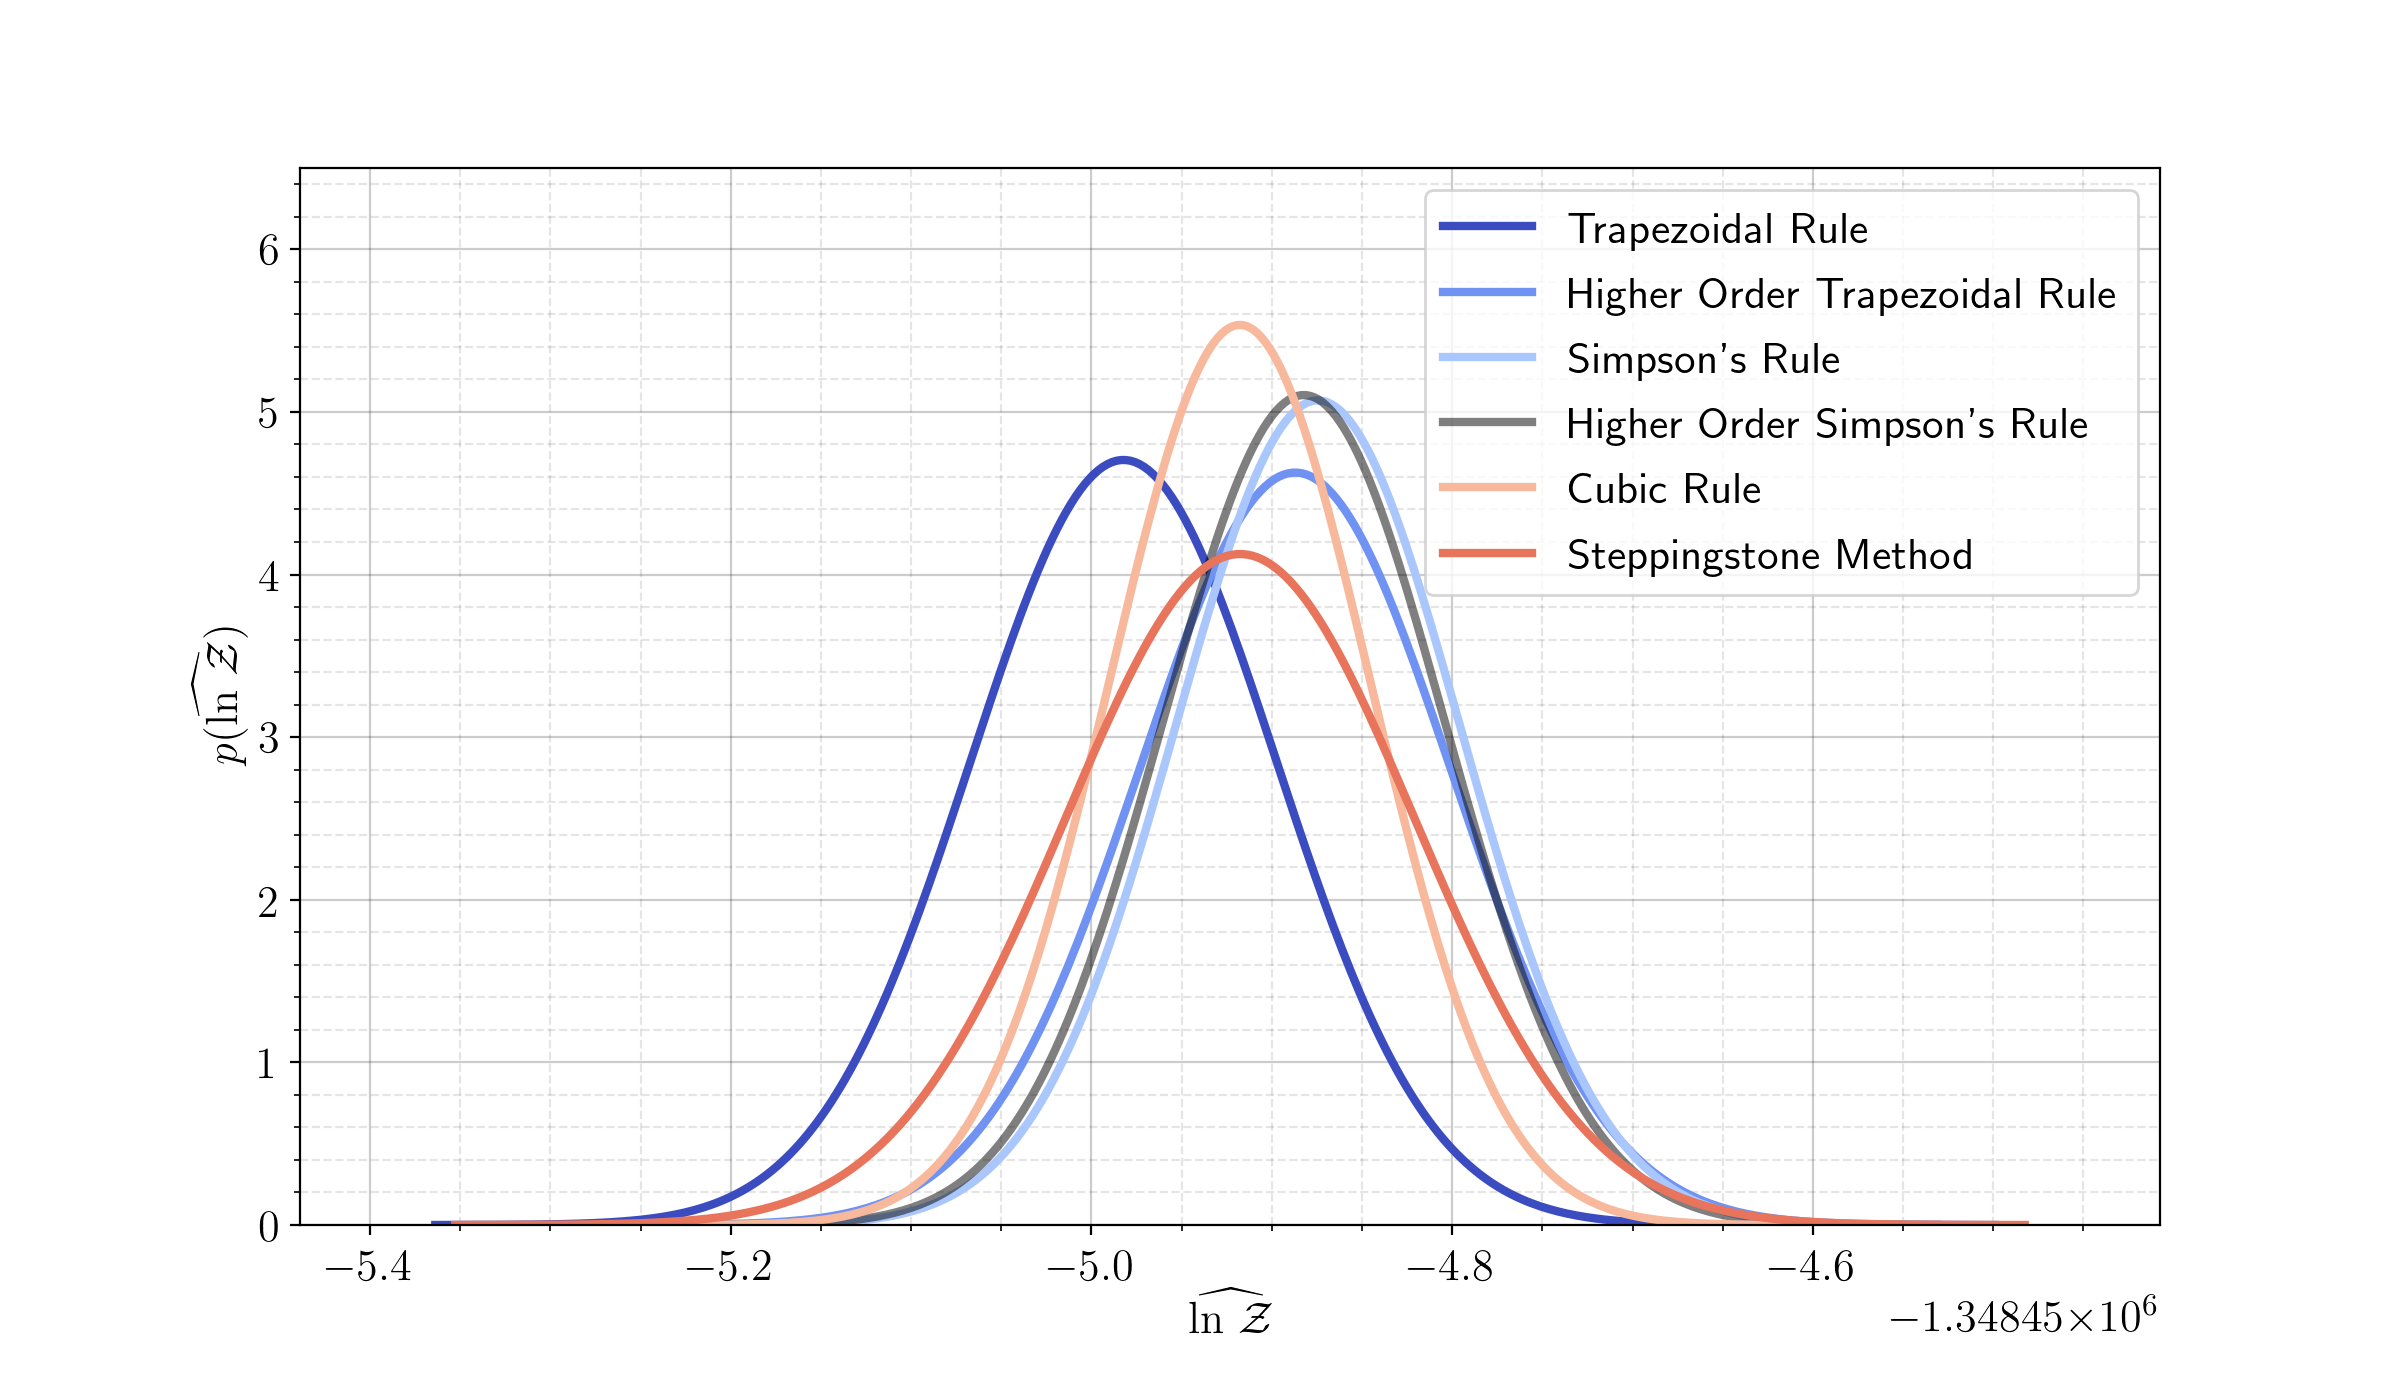
\includegraphics[width=0.9\columnwidth]{figs/chapter6/multi_temper_log_z_lsc_sim.png}
\caption{The estimates of the logarithm of the evidence from multi-temper evidence integration methods. We model the logarithm of the evidence as a Gaussian in log-space. These data are for the logarithm of the evidence from the unconstrained $\delta \phi$ prior for the $p$-$g$ mode instability model. The trapezoidal rule estimates the lowest log evidence for this model, and the cubic rule has the smallest estimated statistical error uncertainty (the smallest confidence interval). The mean values of the higher order quadrature rules appear to be closer together to one another than they are to the trapezoidal rule.}
\label{fig:lvc_sim_log_evidence_distr}
\end{figure}

The logarithm of the Bayes factor is the difference of the logarithm of the evidence for one hypothesis and the logarithm of the evidence for another hypothesis:
\begin{equation}\label{eqn:log_bayes_factor}
    \mathrm{ln} \, \mathcal{B}^A_B = \mathrm{ln} \, \mathcal{Z}_{\mathrm{A}} - \mathrm{ln} \, \mathcal{Z}_{\mathrm{B}}
\end{equation}
However, since we treat $\mathrm{ln} \, \mathcal{Z}_{\mathrm{A}}$ as a random variable who's true value is unknown and so we must deal with the uncertainty in $\widehat{\mathrm{ln} \, \mathcal{Z}_{\mathrm{A}}}$. The logarithm of the Bayes factor then becomes the difference between two probability distribution functions. This can be solved via convolution and has been solved for the Gaussian case~\citep{bromiley2003products}. Thus the resultant $\widehat{\mathrm{ln} \, \mathcal{B}^A_B}$ is itself a Gaussian distribution function with mean $\mu_{\widehat{\mathrm{ln} \, \mathcal{B}^A_B}} = \mu_{\widehat{\mathrm{ln} \, \mathcal{Z}_A}} - \mu_{\widehat{\mathrm{ln} \, \mathcal{Z}_B}}$ and standard deviation $\sigma_{\widehat{\mathrm{ln} \, \mathcal{B}^A_B}} = \sqrt{\sigma_{\widehat{\mathrm{ln} \, \mathcal{Z}_A}}^2 + \sigma_{\widehat{\mathrm{ln} \, \mathcal{Z}_B}}^2 }$~\citep{bromiley2003products}. This thus gives us the following expression for the distribution function that describes our uncertainty on the logarithm of the Bayes factor:
\begin{equation}\label{eqn:p_log_b}
    p(\widehat{\mathrm{ln} \, \mathcal{B}^A_B}) = \left(\frac{1}{\sqrt{2 \pi \sigma_{\widehat{\mathrm{ln} \, \mathcal{B}^A_B}}}} \right) \mathrm{exp} \left \{-\frac{\left(\widehat{\mathrm{ln} \, \mathcal{B}^A_B} - \mu_{\widehat{\mathrm{ln} \, \mathcal{B}^A_B})}\right)^2} {2 \sigma^2_{\widehat{\mathrm{ln} \, \mathcal{B}^A_B}}}  \right\}.
\end{equation}

The expression in Eq.~(\ref{eqn:p_log_b}) is a Gaussian distribution function in $\widehat{\mathrm{ln} \, \mathcal{B}^A_B}$, but we often prefer to know the estimate on $\mathcal{B}^A_B$ and so we must transform coordinates. This transformation of coordinates, fortunately, is a well-known distribution called the log-normal distribution and it is able to be described in terms of the coordinates used in Eq.~(\ref{eqn:p_log_b}). Below we write out our log-normal probability distribution function for $\widehat{\mathcal{B}^A_B}$:
\begin{equation}
    p(\widehat{\mathcal{B}^A_B}) = \frac{1}{\widehat{\mathcal{B}^A_B} \, \sigma_{\widehat{\mathrm{ln} \, \mathcal{B}^A_B}}} \frac{1}{2\pi} \mathrm{exp} \left \{-\frac{\left(\mathrm{ln} \, \widehat{\mathcal{B}^A_B} - \mu_{\widehat{\mathrm{ln} \, \mathcal{B}^A_B})}\right)^2} {2 \sigma^2_{\widehat{\mathrm{ln} \, \mathcal{B}^A_B}}}  \right\}.
\end{equation}
This is the implementation that we have used to represent that Bayes factor in this study. It is worth noting that for a sufficiently small standard deviation on the logarithm of the Bayes factor, the probability of the distribution function will look approximately Gaussian in shape. One useful property of the log-normal Bayes factor distribution is that the median of the log-normal Bayes factor distribution is identical to the point-estimate Bayes factor, $\mathcal{B}^A_B = \mathrm{exp} \left[\mathrm{ln} \, \mathcal{Z}_{\mathrm{A}} - \mathrm{ln} \, \mathcal{Z}_{\mathrm{B}} \right]$. Note, that the expectation value (mean) of $\mathcal{B}^A_B$ is always right-skewed of the median, while the mode of the distribution is left-skewed relative to the median. Large standard deviations on the logarithm of the evidence will create very long tails for the distribution of the Bayes factor, which can make decision-making on Bayes factors more risky. Future studies should consider limiting the error on the logarithm of the evidence to mitigate the larger error on the Bayes factor.

Our Bayes factor estimation from $6$ multi-tempered estimators on the logarithm of the Bayes factor can be seen in Fig.~\ref{fig:lvc_sim_uni_ceos_bayes_distr} when comparing the hypothesis on $p$-$g$ mode instability for the unconstrained $\delta \phi$ prior to the hypothesis presented in~\cite{de2018tidal} for the uniform mass prior with a common equation of state constraint. The different methods appear to give similar probability distributions on the Bayes factor. Those estimators with large standard deviations in $\mathrm{log} \, \mathcal{B}$ have tails that skew towards a Bayes factor of unity.

Another approach to Bayes factor uncertainty estimation that is less mathematical and easier to gain wrap one's head around is to draw random samples from the Gaussian distribution for the logarithm of the evidence for a particular hypothesis. Subtract the random samples from one another to generate a set of samples for the logarithm of the Bayes factor. Then finally exponentiate the random samples to arrive at a set of samples for the Bayes factor. Finally, create a histogram of the samples to estimate the underlying uncertainty in our Bayes factor estimation. For a sufficiently large number of samples ($\sim \mathcal{O}(10^6)$) the estimate will be very close to the log-normal distribution. We have rigorously checked this through both methods and they agree very well.

\begin{figure}[th]
\centering
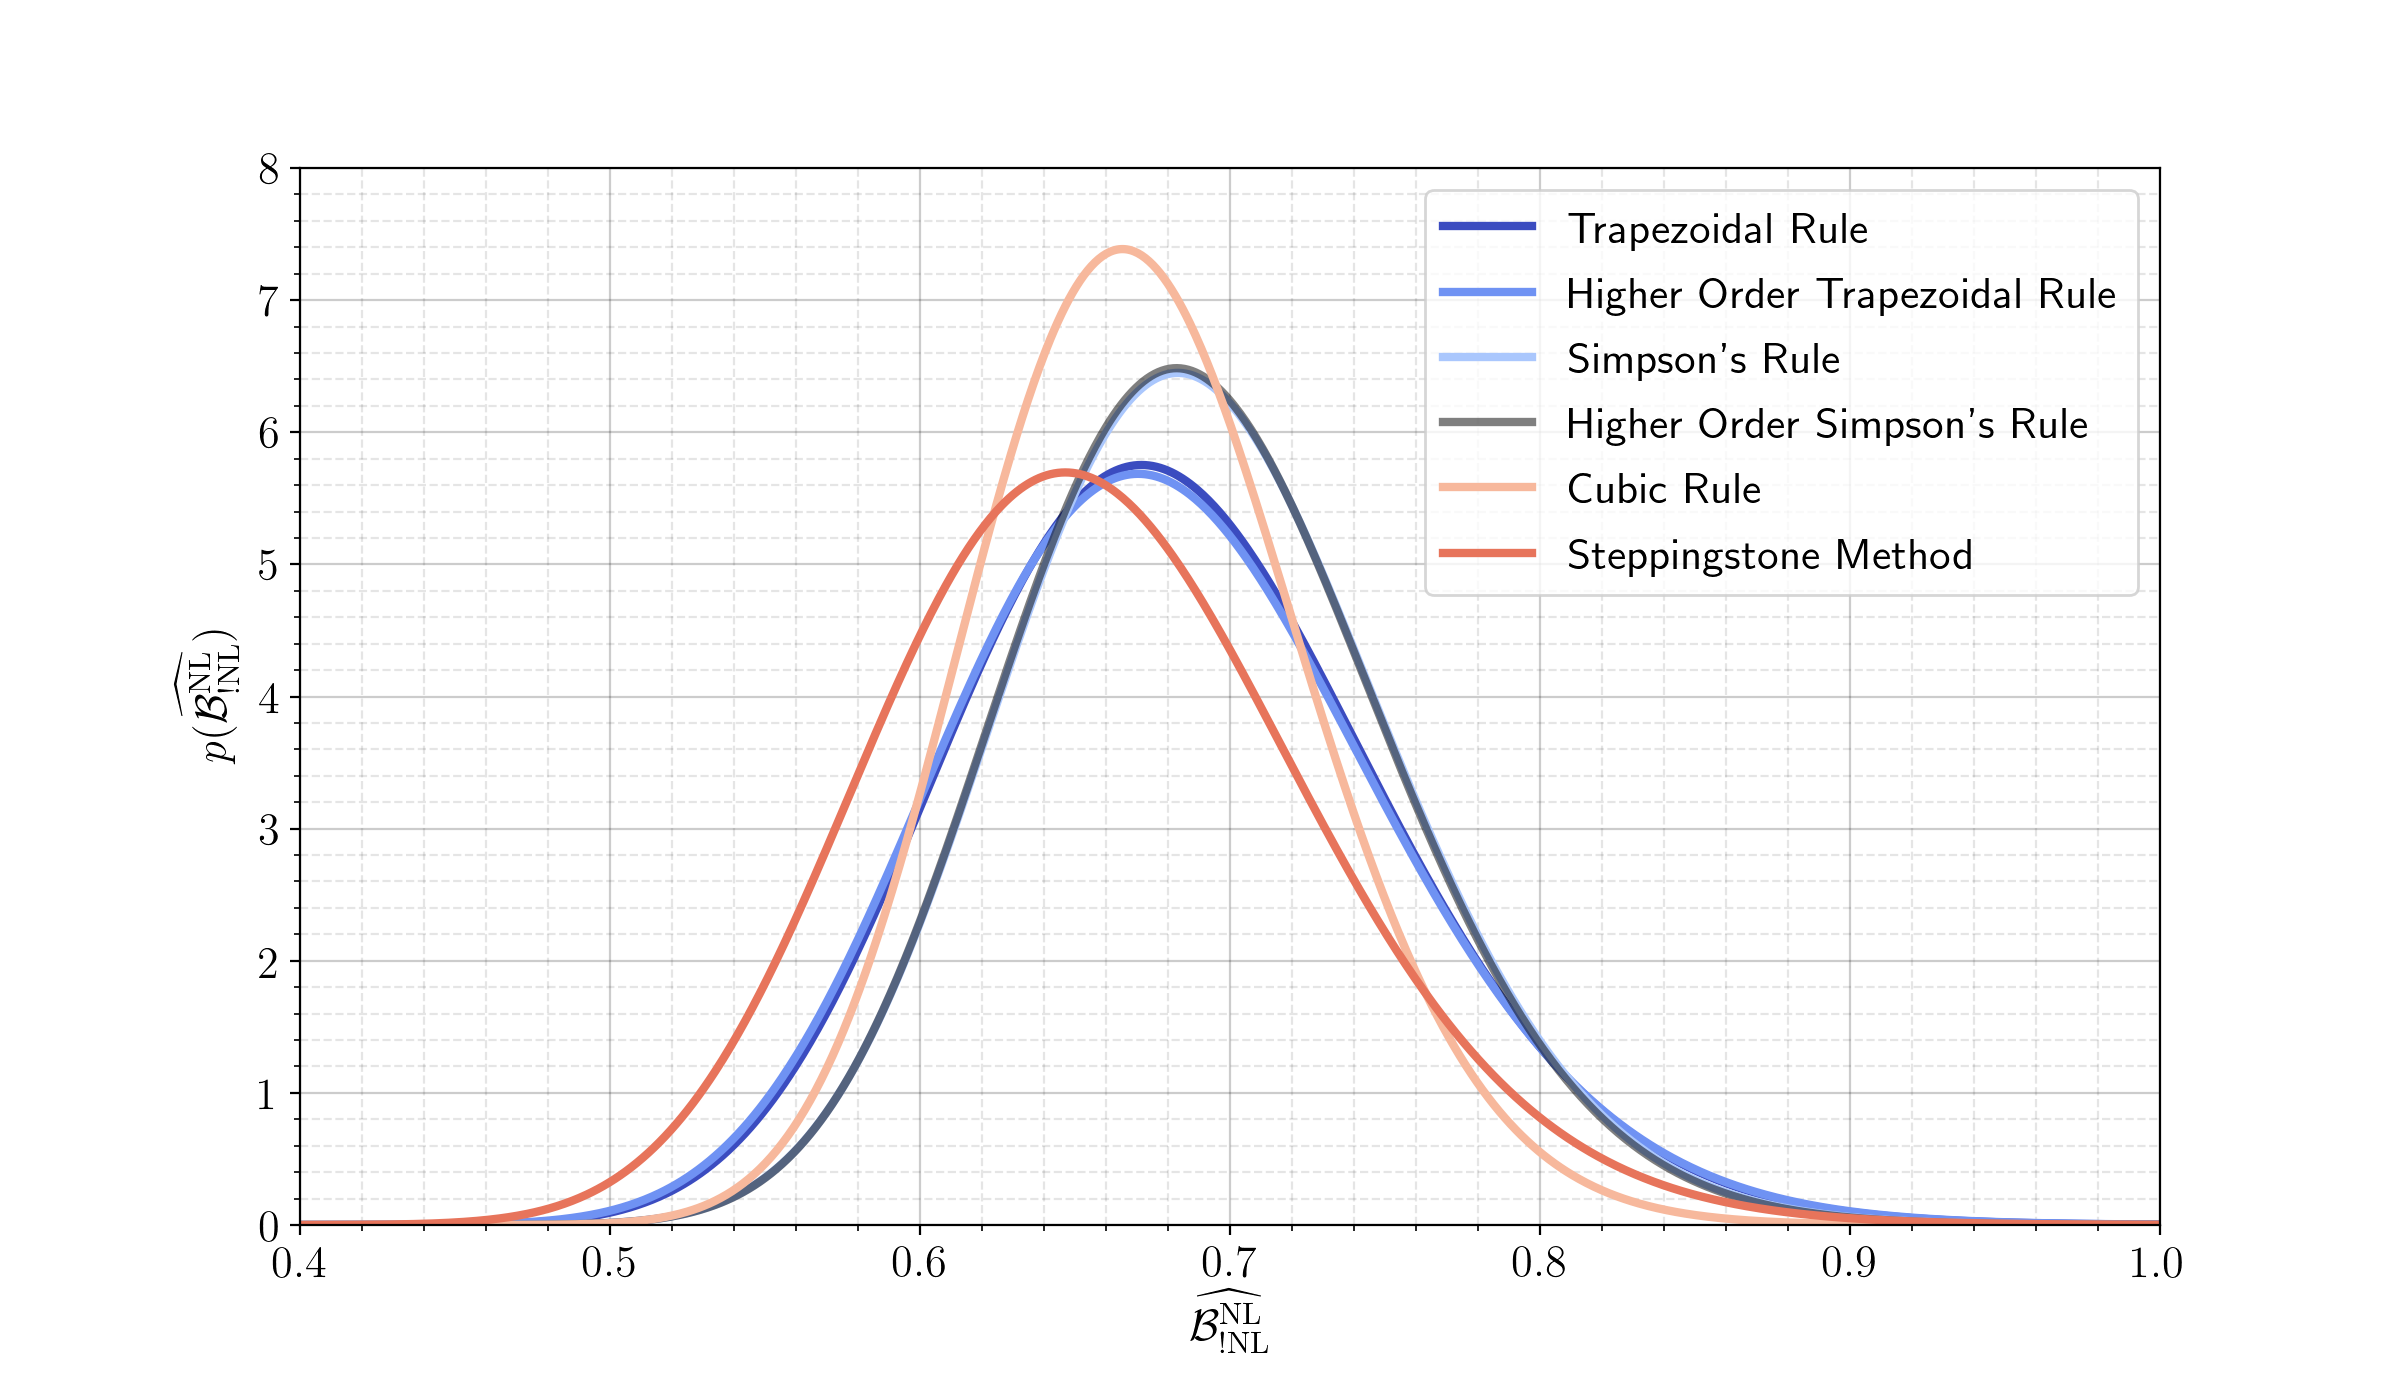
\includegraphics[width=0.9\columnwidth]{figs/chapter6/multi_temper_bayes_lsc_sim_uni_ceos.png}
\caption{The distribution for the Bayes factor for nonlinear tides from $p$-$g$ mode instability from the unconstrained $\delta \phi$ prior relative to the uniform mass, common equation of state prior from~\cite{de2018tidal} under the assumption that the logarithm of the evidence for each model is well approximated by a Gaussian distribution.  but our method is sufficiently accurate in the high-sample limit. When the uncertainty on the logarithm of the evidences in the Bayes factor estimation are sufficiently small, the Bayes factor distribution is approximately normal in shape, but formally they are log-normal distributions.}
\label{fig:lvc_sim_uni_ceos_bayes_distr}
\end{figure}

The Bayes factors for all hypotheses using all of the multi-tempered methods can be seen in Table~\ref{table:Bayes}. The median values of the Bayes factors range between roughly $0.63$ and $0.76$, with the $5^{\mathrm{th}}$ and $95^{\mathrm{th}}$ percentile interval being  around $\pm 0.1$ with a skew towards Bayes factors of $1$. Under a binary choice between the $p$-$g$ mode instability model and the corresponding model without $p$-$g$ mode instability we can calculate a posterior probability of one choice over the other choice. Without giving preference to either model, we can calculate a posterior probability as $p^{\mathrm{NL}}_{\mathrm{!NL}}$ = $\mathcal{B}^{\mathrm{NL}}_{\mathrm{!NL}} / ( 1 + \mathcal{B}^{\mathrm{NL}}_{\mathrm{!NL}})$. Thus, the Bayes factor of $0.63$ corresponds to a posterior probability of $39$ \%  and a Bayes factor of $0.76$ corresponds to a posterior probability of $43$ \%. If we consider the $\pm$ 0.1 ends of the Bayes factor estimation, a Bayes factor of $0.53$ can be interpreted as a posterior probability of $34$\% probability, while a Bayes factor of $0.86$ can be interpreted as the model having a $46$ \% posterior probability. If we consider all models collectively, the posterior probability on any one, particular model reduces significantly.

\begin{table}[ht]
\begin{tabularx}{1.0\textwidth}{l c c c c c c}
\hline\hline
 Hypothesis Tested  & $\mathcal{B}^{\mathrm{NL}}_{\mathrm{!NL}}(A)$  & $\mathcal{B}^{\mathrm{NL}}_{\mathrm{!NL}}(B)$ & $\mathcal{B}^{\mathrm{NL}}_{\mathrm{!NL}}(C)$ & $\mathcal{B}^{\mathrm{NL}}_{\mathrm{!NL}}(D)$ & $\mathcal{B}^{\mathrm{NL}}_{\mathrm{!NL}}(E)$ & $\mathcal{B}^{\mathrm{NL}}_{\mathrm{!NL}}(F)$\\
\hline\hline
$H_1$ (Uniform Mass, $A$, $n$, $f_0$ $\in$ (15, 100) $Hz$), $\delta \phi > 0.1$ &
$0.63^{+0.08}_{-0.07}$ & $0.63^{+0.08}_{-0.07}$ & $0.64^{+0.07}_{-0.06}$ & $0.64^{+0.05}_{-0.05}$ & $0.63^{+0.06}_{-0.06}$ & $0.63^{+0.06}_{-0.06}$ \\ 
\hline 
$H_2$ (Gaussian Mass, $A$, $n$, $f_0$ $\in$ (15, 100) $Hz$), $\delta \phi > 0.1$ &
$0.71^{+0.08}_{-0.07}$ & $0.71^{+0.08}_{-0.07}$ & $0.70^{+0.06}_{-0.06}$ & $0.70^{+0.04}_{-0.04}$ & $0.71^{+0.06}_{-0.06}$ & $0.73^{+0.07}_{-0.07}$ \\ 
\hline
$H_3$ (Uniform Mass, $A$, $n$, $f_0$ $\in$ (15, 800) $Hz$), $\delta \phi > 0.1$ &
$0.64^{+0.09}_{-0.08}$ & $0.64^{+0.09}_{-0.08}$ & $0.64^{+0.08}_{-0.07}$ & $0.64^{+0.06}_{-0.06}$ & $0.64^{+0.06}_{-0.06}$ & $0.63^{+0.09}_{-0.07}$ \\  
\hline
$H_4$ (Gaussian Mass, $A$, $n$, $f_0$ $\in$ (15, 800) $Hz$), $\delta \phi > 0.1$ &
$0.76^{+0.08}_{-0.07}$ & $0.76^{+0.08}_{-0.07}$ & $0.75^{+0.06}_{-0.06}$ & $0.75^{+0.04}_{-0.04}$ & $0.75^{+0.05}_{-0.05}$ & $0.76^{+0.07}_{-0.06}$ \\ 
\hline
$H_5$ (Uniform Mass, $A$, $n$, $f_0$ $\in$ (10, 100) $Hz$) &
$0.68^{+0.12}_{-0.11}$ & $0.68^{+0.13}_{-0.11}$ & $0.69^{+0.11}_{-0.1}$ & $0.69^{+0.1}_{-0.09}$ & $0.67^{+0.1}_{-0.08}$ & $0.65^{+0.13}_{-0.11}$ \\ 
\hline\hline
\end{tabularx}
\caption{The various Bayes factors under different multi-tempered integration methods. The column marked with $\mathcal{B}^{\mathrm{NL}}_{\mathrm{!NL}}(A)$ is the Bayes factor under the thermodynamic integration method using the trapezoid quadrature rule. The $(B)$ column is the Bayes factor from the thermodynamic integration method using the higher-order trapezoid quadrature rule. The $(C)$ column is the Bayes factor from the thermodynamic integration method using Simpson's quadrature rule. The $(D)$ column is the Bayes factor for the thermodynamic integration method using Simpson's higher-order quadrature rule. The $(E)$ column is the Bayes factor for the thermodynamic integration method using a cubic polynomial quadrature rule. And $(F)$ is the Bayes factor from the steppingstone method. The $50^{\mathrm{th}}$ percentile with the $5^{\mathrm{th}}$ and $95^{\mathrm{th}}$ percentiles in the plus and minus superscripts and subscripts, respectively, are shown above.}\label{table:Bayes}
\end{table}

%$0.631831831832^{+0.0774774774775}_{-0.0684684684685}$ & $0.631831831832^{+0.0774774774775}_{-0.0690690690691}$ & $0.637237237237^{+0.0678678678679}_{-0.0612612612613}$ & $0.637237237237^{+0.0528528528529}_{-0.0486486486486}$ & $0.633633633634^{+0.0600600600601}_{-0.0546546546547}$ & $0.633633633634^{+0.0600600600601}_{-0.0546546546547}$ \\ 

%$0.708708708709^{+0.0786786786787}_{-0.0708708708709}$ & $0.709309309309^{+0.0786786786787}_{-0.0714714714715}$ & $0.702102102102^{+0.0630630630631}_{-0.0582582582583}$ & $0.701501501502^{+0.0432432432432}_{-0.0408408408408}$ & $0.710510510511^{+0.0606606606607}_{-0.0564564564565}$ & $0.726726726727^{+0.0744744744745}_{-0.0678678678679}$ \\ 

%$0.637237237237^{+0.0864864864865}_{-0.0762762762763}$ & $0.637837837838^{+0.0870870870871}_{-0.0768768768769}$ & $0.640840840841^{+0.0756756756757}_{-0.0678678678679}$ & $0.640840840841^{+0.0624624624625}_{-0.0570570570571}$ & $0.64024024024^{+0.0642642642643}_{-0.0588588588589}$ & $0.631831831832^{+0.0846846846847}_{-0.0744744744745}$  \\ 

%$0.756156156156^{+0.0780780780781}_{-0.0714714714715}$ & $0.756756756757^{+0.0786786786787}_{-0.0714714714715}$ & $0.753153153153^{+0.0636636636637}_{-0.0582582582583}$ & $0.753153153153^{+0.0402402402402}_{-0.0378378378378}$ & $0.74954954955^{+0.0516516516517}_{-0.0474474474474}$ & $0.75975975976^{+0.0672672672673}_{-0.0618618618619}$  \\ 

%$0.678678678679^{+0.124924924925}_{-0.105705705706}$ & $0.677477477477^{+0.126726726727}_{-0.106306306306}$ & $0.688888888889^{+0.10990990991}_{-0.0948948948949}$ & $0.688288288288^{+0.0984984984985}_{-0.0858858858859}$ & $0.66966966967^{+0.0954954954955}_{-0.0834834834835}$ & $0.654654654655^{+0.126726726727}_{-0.106306306306}$ \\ 

\section{Performance of Savage-Dickey Density Tests}\label{sec:prob_density_estimator_performance}
Below we will enumerate the methods used to conduct the Savage-Dickey density test for finding the Bayes factor of the  on $p$-$g$ mode instability for the unconstrained $\delta \phi$ prior compared to a null-hypothesis, that is a hypothesis where $p$-$g$ mode instability is not modeled. Formally, this is the model presented in~\cite{de2018tidal} for the uniform mass prior with a common equation of state constraint however the Savage-Dickey density test makes no use of the data from~\cite{de2018tidal}. While this may sound somewhat outrageous, we will find that the results generally agree with those found using multi-tempered model selection techniques. The results of all of the Savage-Dickey density tests are collected and summarized in Table~\ref{table:Bayes_sddr}. 

\subsection{Histogram Method}
An elementary method for estimating the probability density function is to histogram the samples and normalize the histogram to integrate to unity. Under this methodology the only relevant parameter to fitting the histogram to the data is the choice of bin-width, sometimes called bandwidth.

Two methods that we have used to try to maximize the fit of the histogram to the data are through the choice of plug-in bin-width algorithms. The algorithms are designed to minimize the error to the histogram density fit to an underlying density function. The first is Scott's rule~\citep{scott1979optimal} and is considered optimal relative to a density function that is normally distributed, and hence the bin-width $h$ is defined as:
\begin{equation}
    h = \frac{3.5 \, \hat{\sigma}}{N^{1/3}}.
\end{equation}
Here $\hat{\sigma}$ represents the sample standard deviation of the data, and $N$ represents the number of samples in the data.

The second method is described in ~\cite{Freedman1981} and makes use of the interquartile range (IQR). The IQR is the difference between the $75^{\mathrm{th}}$ and $25^{\mathrm{th}}$ percentile of the data. The Freedman-Diaconis bin method ~\citep{Freedman1981}, where the bin-width $h$ is:
\begin{equation}
    h = \frac{2 \, \mathrm{IQR}}{N^{1/3}}
\end{equation}
Here $N$ represents the number of samples in the data.

Since the marginal prior (posterior) distribution functions on $A$ are distributed logarithmically, it is convenient to do the density estimation in the variable $\tilde{X} \equiv \mathrm{log}_{10} \, A$. Under this change of variables the marginal prior distribution on $\tilde{X}$ is uniform between $\tilde{X}=-10$ and $\tilde{X}=-5.5$, hence the distribution function is constant over all values of $\tilde{X}$:
\begin{equation}
    \pi\left(\tilde{X}\right) = \frac{1}{\tilde{X}_{max} - \tilde{X}_{min}} = 0.2\overbar{2}, \qquad -10.0 \leq \tilde{X} \leq -5.5
\end{equation}

Using the histogram bin-width rules from above we estimate the marginal posterior probability density at $\tilde{X} = -10.0$. To simulate the variability of the algorithm to the data we resample from the the marginal posterior probability density distribution of $\mathrm{log}_{10} \, A$ via the bootstrap method some $5,000$ times. This gives us a distribution of possible Bayes factor values. We find a $\mathcal{B}^{\mathrm{NL}}_{!\mathrm{NL}} = 0.66^{+0.08}_{-0.07}$ at the $90\%$ confidence interval for Scott's Rule and a $\mathcal{B}^{\mathrm{NL}}_{!\mathrm{NL}} = 0.66^{+0.08}_{-0.06}$ at the $90\%$ confidence interval for the Freedman-Diaconis Rule. For a comparison of the density estimates for the marginal posterior probability density on $\mathrm{log}_{10} \, A$ see Fig.~\ref{fig:density_estimators}. The Bayes factor uncertainty distribution is shown, in comparison to the other density estimators and the thermodynamic integration method uner the higher-order trapezoidal rule, in Fig.~\ref{fig:sddr_bayes_factor_comparisons}.

\subsection{Gaussian Kernel Density Estimator}
We use a Gaussian kernel density estimator available in the Python package GetDist~\citep{lewis2015getdist}. GetDist is a Python package intended to accurately estimate the underlying one-dimensional and two-dimensional posterior probability distribution functions from a Bayesian MCMC analysis. A rough understanding of a Gaussian kernel density estimator is that it uses small truncated-Gaussian distributions centered at samples of the data and combines the sum of the distributions into a smooth probability distribution function.

The advantage that GetDist offers over other Gaussian kernel density estimators is that it comes with robust linear-boundary bias corrections to the Gaussian kernel. Sharp boundaries on the distribution function are known to cause bias to the probability distribution function estimation for Gaussian kernel density estimators~\citep{lewis2015getdist}, and the Savage-Dickey density ratio method in this application requires us to know the density of the posterior distribution function at the boundary. GetDist uses an asymmetric linear addition to the kernel at the boundaries which helps to ameliorate some of the boundary bias. There are additional bias-correction and bandwidth optimization algorithms in the routine that help improve the accuracy of the density estimation. See~\cite{lewis2015getdist} for the full details.

We follow the same procedure in estimating the posterior probability density of $A$ at $10^{-10}$ as in the histogram method. We resample the posterior distribution through the bootstrap method to generate $5,000$ estimates of $\mathcal{P}(A =10^{-10}|\mathbf{d})$. This then yields an estimate of the Bayes factor at the $90\%$ confidence level of $\mathcal{B}^{\mathrm{NL}}_{!\mathrm{NL}} = 0.66^{+0.13}_{-0.1}$. For a comparison of the density estimates for the marginal posterior probability density on $\mathrm{log}_{10} \, A$ see Fig.~\ref{fig:density_estimators}. The Bayes factor uncertainty distribution is shown, in comparison to the other density estimators and the thermodynamic integration method under the higher-order trapezoidal rule, in Fig.~\ref{fig:sddr_bayes_factor_comparisons}.

\subsection{Logspline Density Estimator}
In the logspline density estimator of~\cite{stone1997polynomial} a univariate log-probability density is modeled by a cubic spline. The algorithm places knots of a cubic spline in an algorithmic fashion and uses an internal likelihood function to find a maximum likelihood number of knots (and placement) to use. Internal to the software package is a Bayesian model-selection routine based on the Akaike Information Criterion (AIC)~\citep{akaike1981likelihood} and the Bayesian Information Criterion (BIC)~\citep{schwarz1978estimating} to both ensure goodness of fit and to avoid over-fitting to the data. The details of the procedure are sophisticated and beyond the scope of this study. We utilize the maximum likelihood fit to the probability distribution function from the packages' model selection routine. We note that using the maximum likelihood fit is not very risky as the likelihood for other values of knot and knot placement as given from the package's fit routine provide posterior density estimates that are almost identical to the maximum likelihood fit.

We use the same bootstrap method outlined above to estimate the variability of the logspline algorithm relative to the variability of the data. We find an estimate of the Bayes factor at the $90\%$ confidence level of $\mathcal{B}^{\mathrm{NL}}_{!\mathrm{NL}} = 0.63^{+0.06}_{-0.05}$. For a comparison of the density estimates for the marginal posterior probability density on $\mathrm{log}_{10} \, A$ see Fig.~\ref{fig:density_estimators}. The Bayes factor uncertainty distribution is shown, in comparison to the other density estimators and the thermodynamic integration method under the higher-order trapezoidal rule, in Fig.~\ref{fig:sddr_bayes_factor_comparisons}.

\begin{figure}[th]
\centering
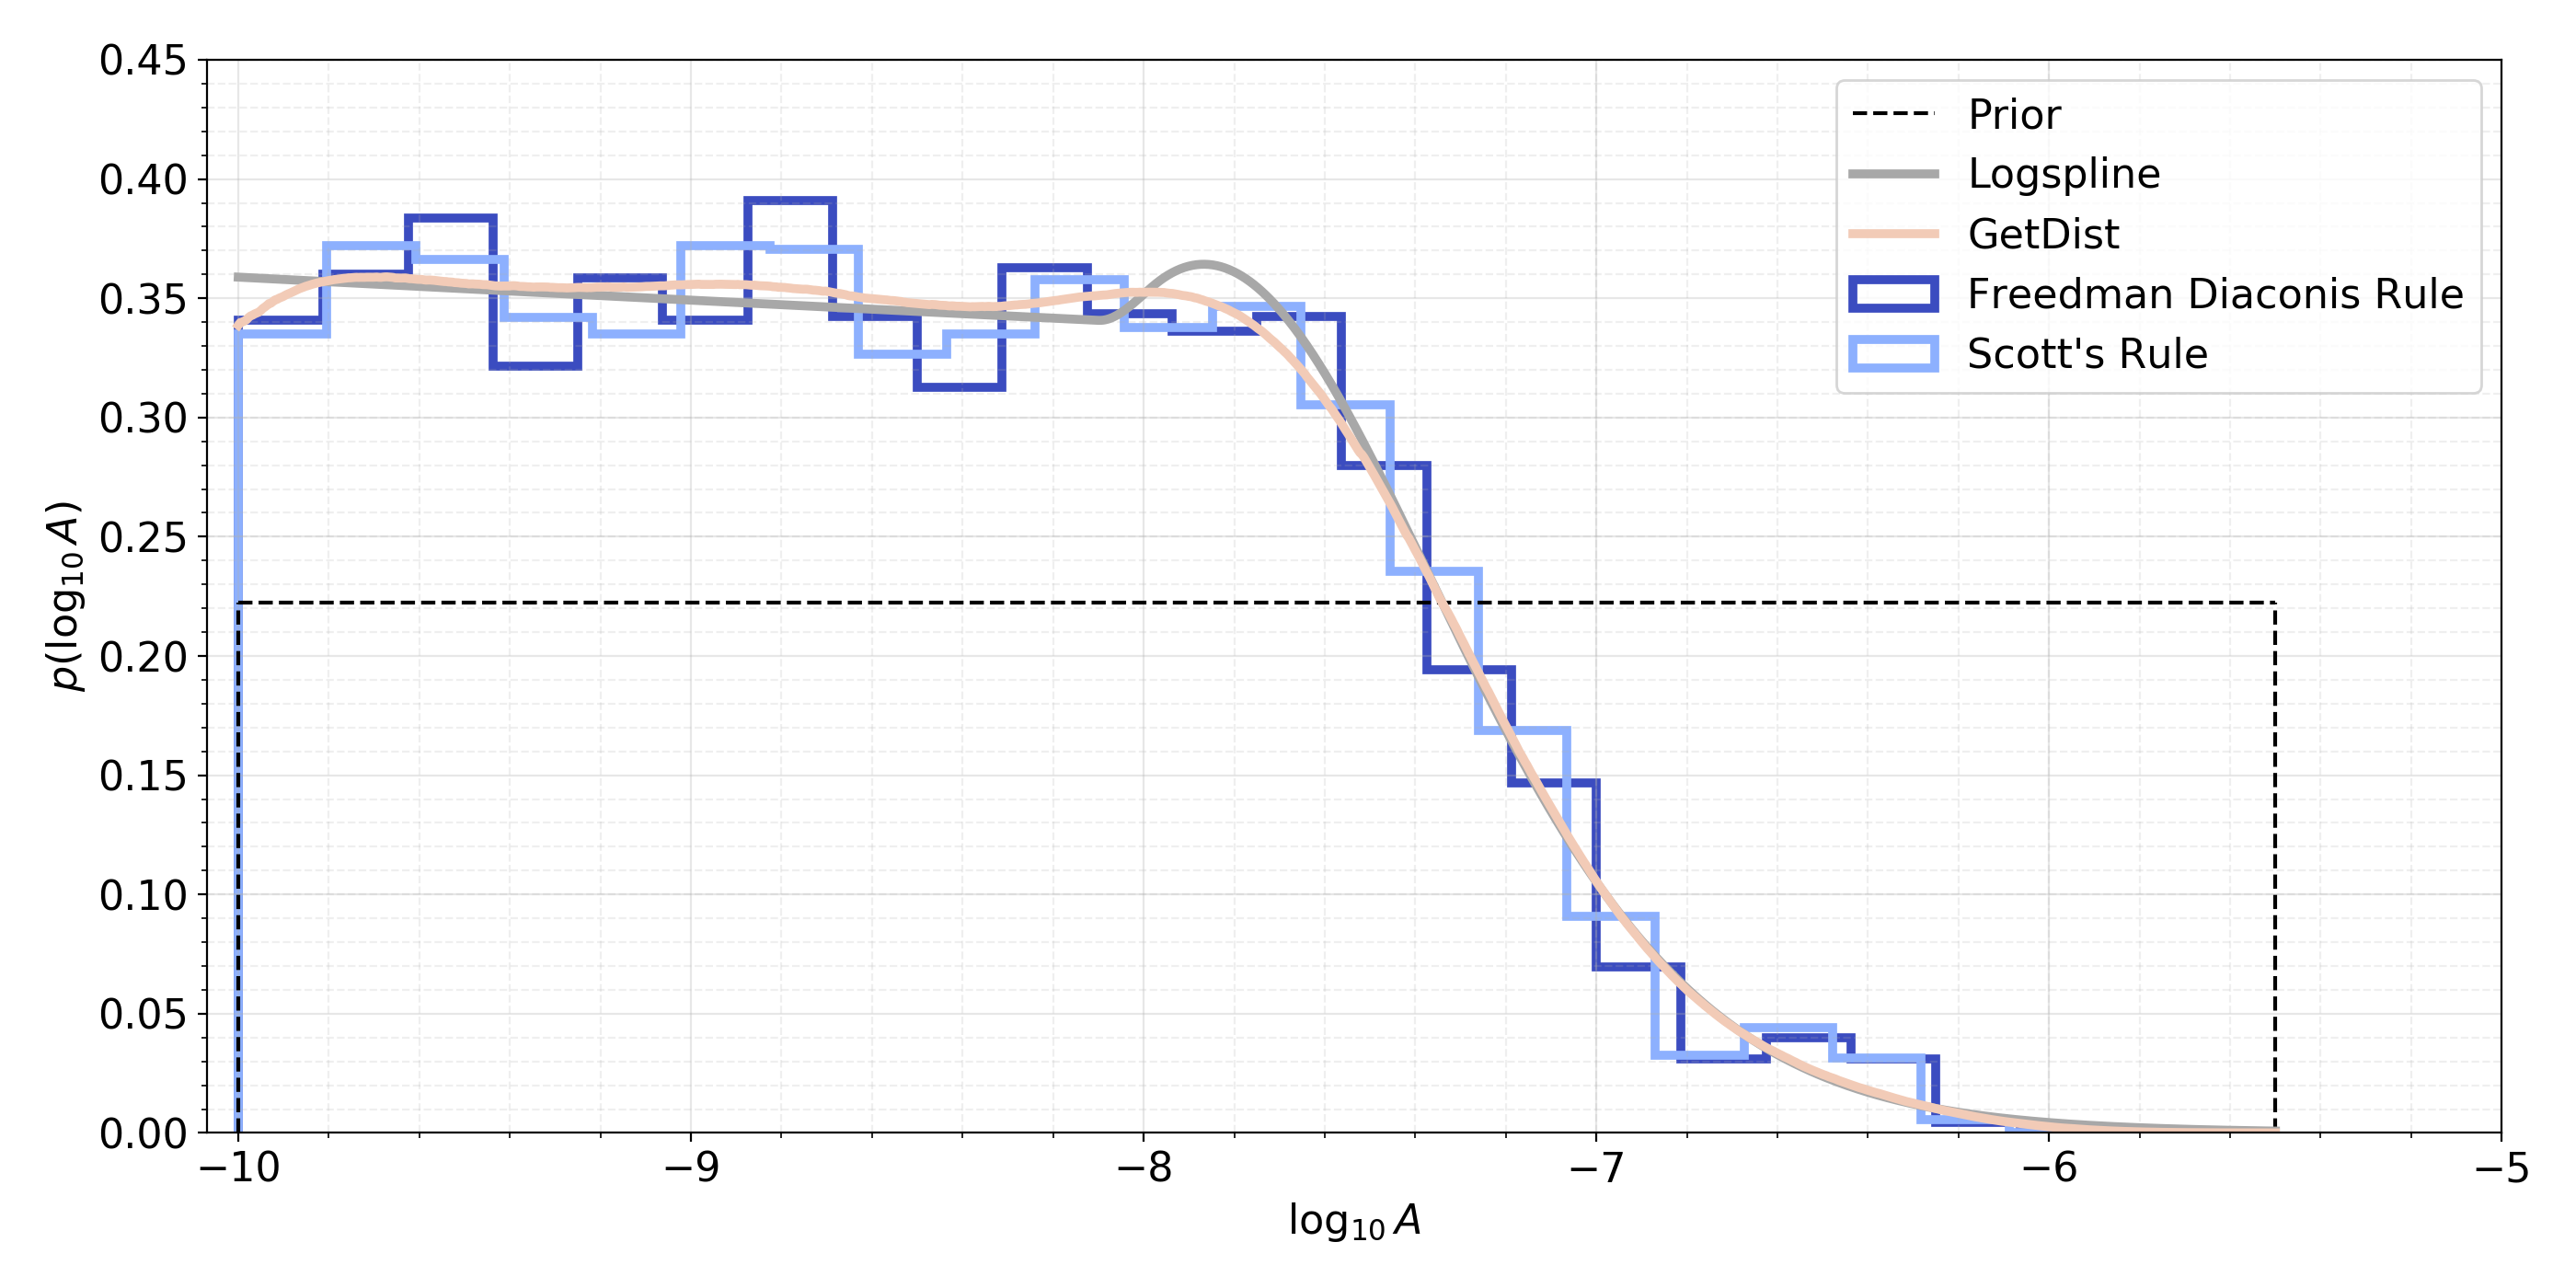
\includegraphics[width=0.9\columnwidth]{figs/chapter6/prior_posterior_sddr.png}
\caption{The prior and posterior density estimations from different density estimators for the parameter $\mathrm{log}_{10} \, A$. The prior density is uniform in $\mathrm{log}_{10}$ and is $0.\overbar{2}$. Posterior Logspline is the density estimation under the logspline density estimator, and it is notable that it tends to estimate the posterior density at $\mathrm{log}_{10} \, A = -10$ more highly than the other estimators. If this is systematically true, then the Bayes factor from the logspline density estimator will be smaller than the other estimators. Posterior GetDist is the Gaussian kernel density estimator described in the Python GetDist package. Posterior FD and Scott are the histogram methods under the Freedman-Diaconis binning rule and Scott's binning rule, respectively. We can see here that there is some \textit{wasted} prior space at large $\mathrm{log}_{10} A$. THe posterior density might more closely match the prior density if we restricted our prior density to smaller $\mathrm{log}_{10} A$.}
\label{fig:density_estimators}
\end{figure}

\begin{figure}[th]
\centering
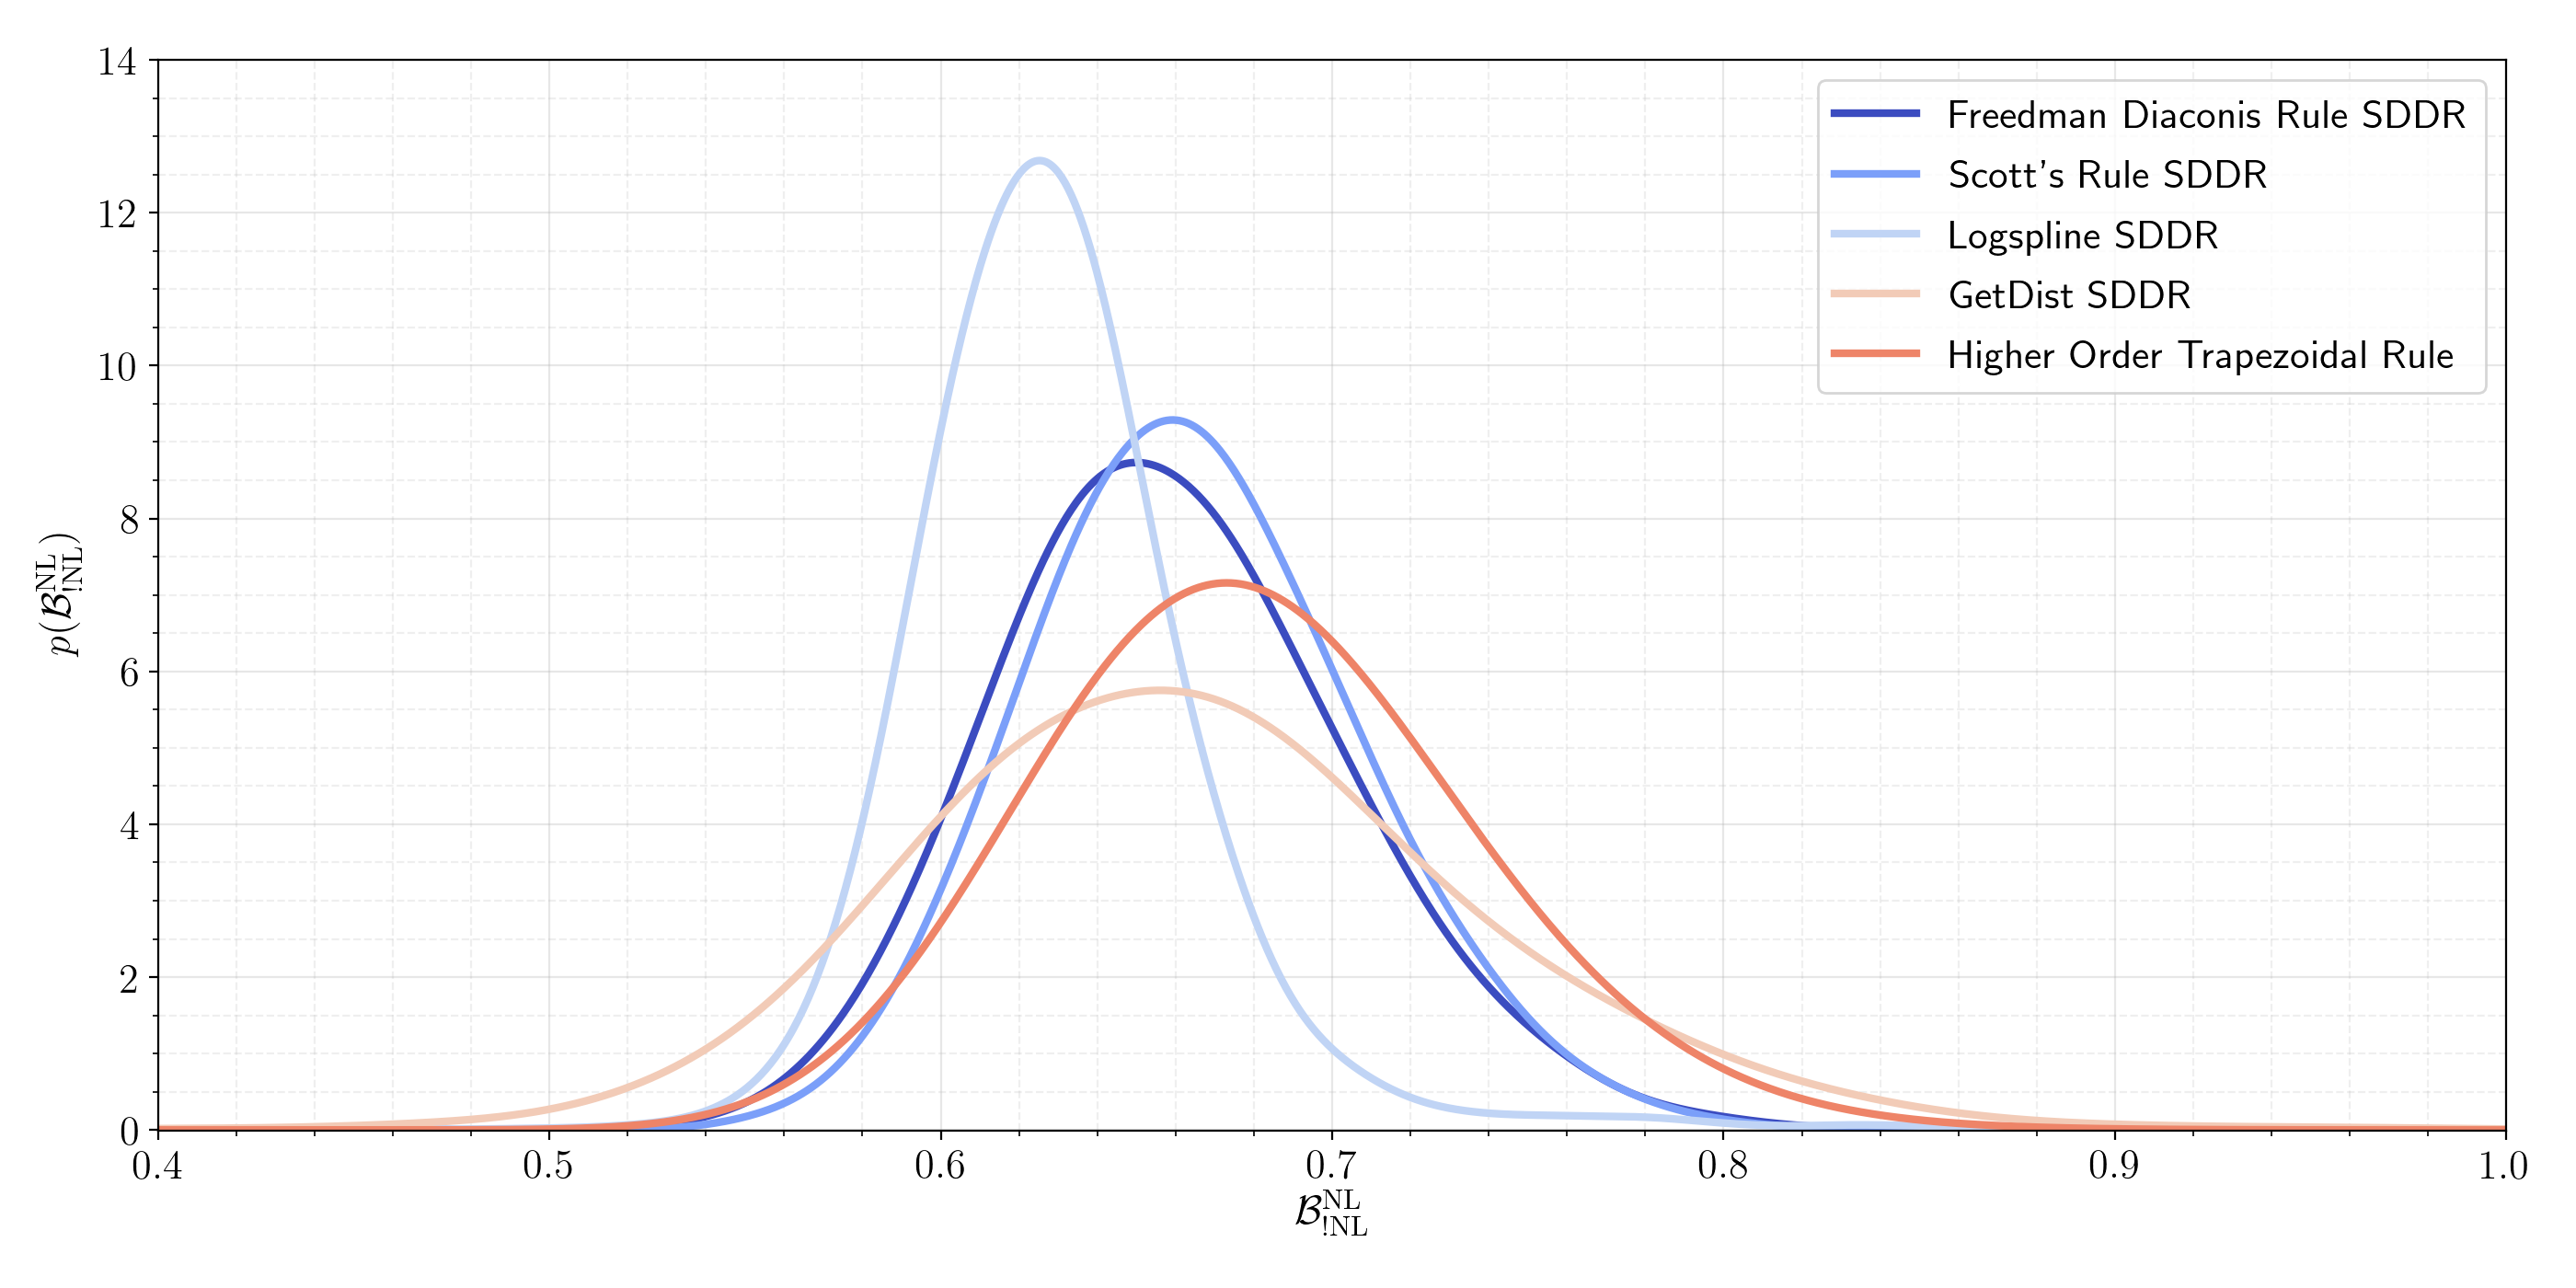
\includegraphics[width=0.9\columnwidth]{figs/chapter6/sddr_bayes_factor.png}
\caption{A comparison of the Bayes factor estimates for $p$-$g$ mode instability with the permissive prior on $\delta \phi$ vs no $p$-$g$ mode instability from different methods. Here, SDDR refers to the Savage Dickey density ratio test for each corresponding estimator technique. We compare these results to the higher order trapezoidal rule from thermodynamic integration. The other multi-tempered Bayes factors are comparable to the one shown here and so are not displayed. The estimates generally agree and if required we could marginalize over the method for calculating the Bayes factor to report one single value.}
\label{fig:sddr_bayes_factor_comparisons}
\end{figure}

\begin{table}[ht]
\begin{tabularx}{1.0\textwidth}{l c c c c}
\hline\hline
 Hypothesis Tested  & $\mathcal{B}^{\mathrm{NL}}_{\mathrm{!NL}}$(FD)  & $\mathcal{B}^{\mathrm{NL}}_{\mathrm{!NL}}$(Scott) & $\mathcal{B}^{\mathrm{NL}}_{\mathrm{!NL}}$(Gaussian KDE) & $\mathcal{B}^{\mathrm{NL}}_{\mathrm{!NL}}$(Logspline)\\
\hline\hline
$H_5$ (Uniform Mass, $A$, $n$, $f_0$ $\in$ (10, 100) $Hz$) &
$0.66^{+0.08}_{-0.07}$ & $0.66^{+0.08}_{-0.07}$ & $0.66^{+0.13}_{-0.1}$ & $0.63^{+0.06}_{-0.05}$ \\
\hline\hline
\end{tabularx}
\caption{The various Bayes factors from the Savage-Dickey Density Ratio test under different density estimators. The column marked with $\mathcal{B}^{\mathrm{NL}}_{\mathrm{!NL}}$(FD) is the Bayes factor from the Freedman Diaconis histogram binning rule. The $\mathcal{B}^{\mathrm{NL}}_{\mathrm{!NL}}$(Scott) column is the Bayes factor estimate under Scott's histogram binning rule. The $\mathcal{B}^{\mathrm{NL}}_{\mathrm{!NL}}$(Gaussian KDE) column is the Bayes factor estimate when using the Gaussian kernel density estimator with linear boundary bias corrections as found in the GetDist Python package. The column denoted as  $\mathcal{B}^{\mathrm{NL}}_{\mathrm{!NL}}$(Logspline) is the Bayes factor estimate when using the logspline density estimator. The $50^{\mathrm{th}}$ percentile with the $5^{\mathrm{th}}$ and $95^{\mathrm{th}}$ percentiles in the plus and minus superscripts and subscripts, respectively.}\label{table:Bayes_sddr}
\end{table}

\section{Can we improve the chirp mass measurement with an independent EM Observation?}
We noted in the introduction that we would require a strong constraint on the chirp mass independent of the gravitational wave data to mitigate the parameter degeneracy from the $p$-$g$ mode instability. Here we make a rough quantitative analysis of how tight an electromagnetic observation would have to constrain the chirp mass. To do so we must consider the joint posterior distribution, $\mathcal{P}(\mathcal{M} \, | \,  \mathbf{d_{GW}}, \mathbf{d_{EM}})$, from two statistically independent data sets, the gravitational wave data $\mathbf{d_{GW}}$, and a mock electromagnetic data set $\mathbf{d_{EM}}$. We must then define a (hyper) prior on the chirp mass that bridges the measured likelihood of the chirp mass for each data set to the posterior distribution. This expression looks as follows:
\begin{equation}
    \mathcal{P}(\mathcal{M} \, | \,  \mathbf{d_{GW}}, \mathbf{d_{EM}}) = \frac{\pi(\mathcal{M})}{\mathcal{Z}(\mathbf{d_{GW}}, \mathbf{d_{EM}})}  \,  \mathcal{L}(\mathbf{d_{GW}}, \mathbf{d_{EM}} \, | \, \mathcal{M}) = \frac{\pi(\mathcal{M})}{\mathcal{Z}(\mathbf{d_{GW}}, \mathbf{d_{EM}})} \, \mathcal{L}(\mathbf{d_{GW}} \, | \, \mathcal{M}) \, \mathcal{L}(\mathbf{d_{EM}} \, | \, \mathcal{M}).
\end{equation}
The separation of $\mathcal{L}(\mathbf{d_{GW}}, \mathbf{d_{EM}} \, | \, \mathcal{M}) = \mathcal{L}(\mathbf{d_{GW}} \, | \, \mathcal{M}) \, \mathcal{L}(\mathbf{d_{EM}} \, | \, \mathcal{M})$ follows from the two being statistically independent measurements of the chirp mass of GW170817. Here, $\mathcal{Z}(\mathbf{d_{GW}}, \mathbf{d_{EM}})$ is the normalizing constant that maintains the equality, which is easy to solve for computationally for a one parameter model. We will call this normalizing constant $c$ from now on. Finding the marginal likelihood of $\mathcal{L}(\mathbf{d_{GW}} \, | \, \mathcal{M})$ given all of the parameters in the analysis would be a prohibitively difficult difficult to construct without the MCMC methods described here for calculating the likelihood marginalized over all parameters. However, an application of Bayes' theorem reduces this problem to one that we can solve from the data in hand. Consider that $\mathcal{L}(\mathbf{d_{GW}} \, | \, \mathcal{M}) = \mathcal{P}(\mathcal{M} \, | \, \mathbf{d_{GW}}) / \pi_{\mathrm{GW}} (\mathcal{M})$ for the properly normalized marginal posterior and prior distributions on the chirp mass.

\begin{equation}
    \mathcal{P}(\mathcal{M} \, |  \, \mathbf{d_{GW}}, \mathbf{d_{EM}}) = \frac{\pi(\mathcal{M})}{c} \times \frac{\mathcal{P}(\mathcal{M} \, | \, \mathbf{d_{GW}})}{\pi_{\mathrm{GW}}(\mathcal{M})} \times \frac{\mathcal{P}(\mathcal{M} \, | \, \mathbf{d_{EM}})}{\pi_{\mathrm{EM}}(\mathcal{M})}
\end{equation}

Now, since we don't have a real posterior distribution from electromagnetic data on hand we make a simple assumption, $\mathcal{P}(\mathcal{M} | \mathbf{d_{EM}})$. We let the hyper prior $\pi(\mathcal{M})$ equal to the $\pi_{\mathrm{GW}}(\mathcal{M})$ and equal to our mock-analysis $\pi_{\mathrm{EM}}(\mathcal{M})$. These priors are uniform in chirp mass in the detector fram between $\mathcal{M} \in (1.1876, 1.2076)$. Now, let $\mathcal{P}(\mathcal{M} | \mathbf{d_{EM}})$ be a Gaussian distribution with mean value $\mu$ equivalent to the gravitational wave posterior mode of the chirp mass given a non p-g mode hypothesis. Now, we ask what is the standard deviation $\sigma$ of $\mathcal{P}(\mathcal{M} | \mathbf{d_{EM}})$ required to regulate the p-g mode inferred marginal posterior distribution on the chirp mass so that it \textit{looks} more like the marginal posterior distribution on the chirp mass from the null hypothesis? We solve this computationally for the unconstrained prior on $\delta \phi$ in the $p$-$g$ mode analysis and for the uniform mass distribution with common equation of state constraint from~\cite{de2018tidal}. The normalizing constant $c$ is solved via a fine-grid trapezoidal rule to normalize the posterior to unity. The net result is in Fig.~\ref{fig:em_posterior_analysis} where we find that an electromagnetic observer would need a constraint on $\sigma_{\mathcal{M}} < 0.0001 M_{\odot}$. This corresponds to a measurement error less than $0.008~\%$, well outside the realm of current methods.

One might improve on this simple heuristic by using the marginal chirp mass distribution when marginalizing over all $p$-$g$ mode models and then comparing it to the marginal chirp mass distribution when marginalizing over all models in~\cite{de2018tidal}. But the result would be qualitatively identical and so for simplicity we neglect this possible improvement.

\begin{figure}[th]
\centering
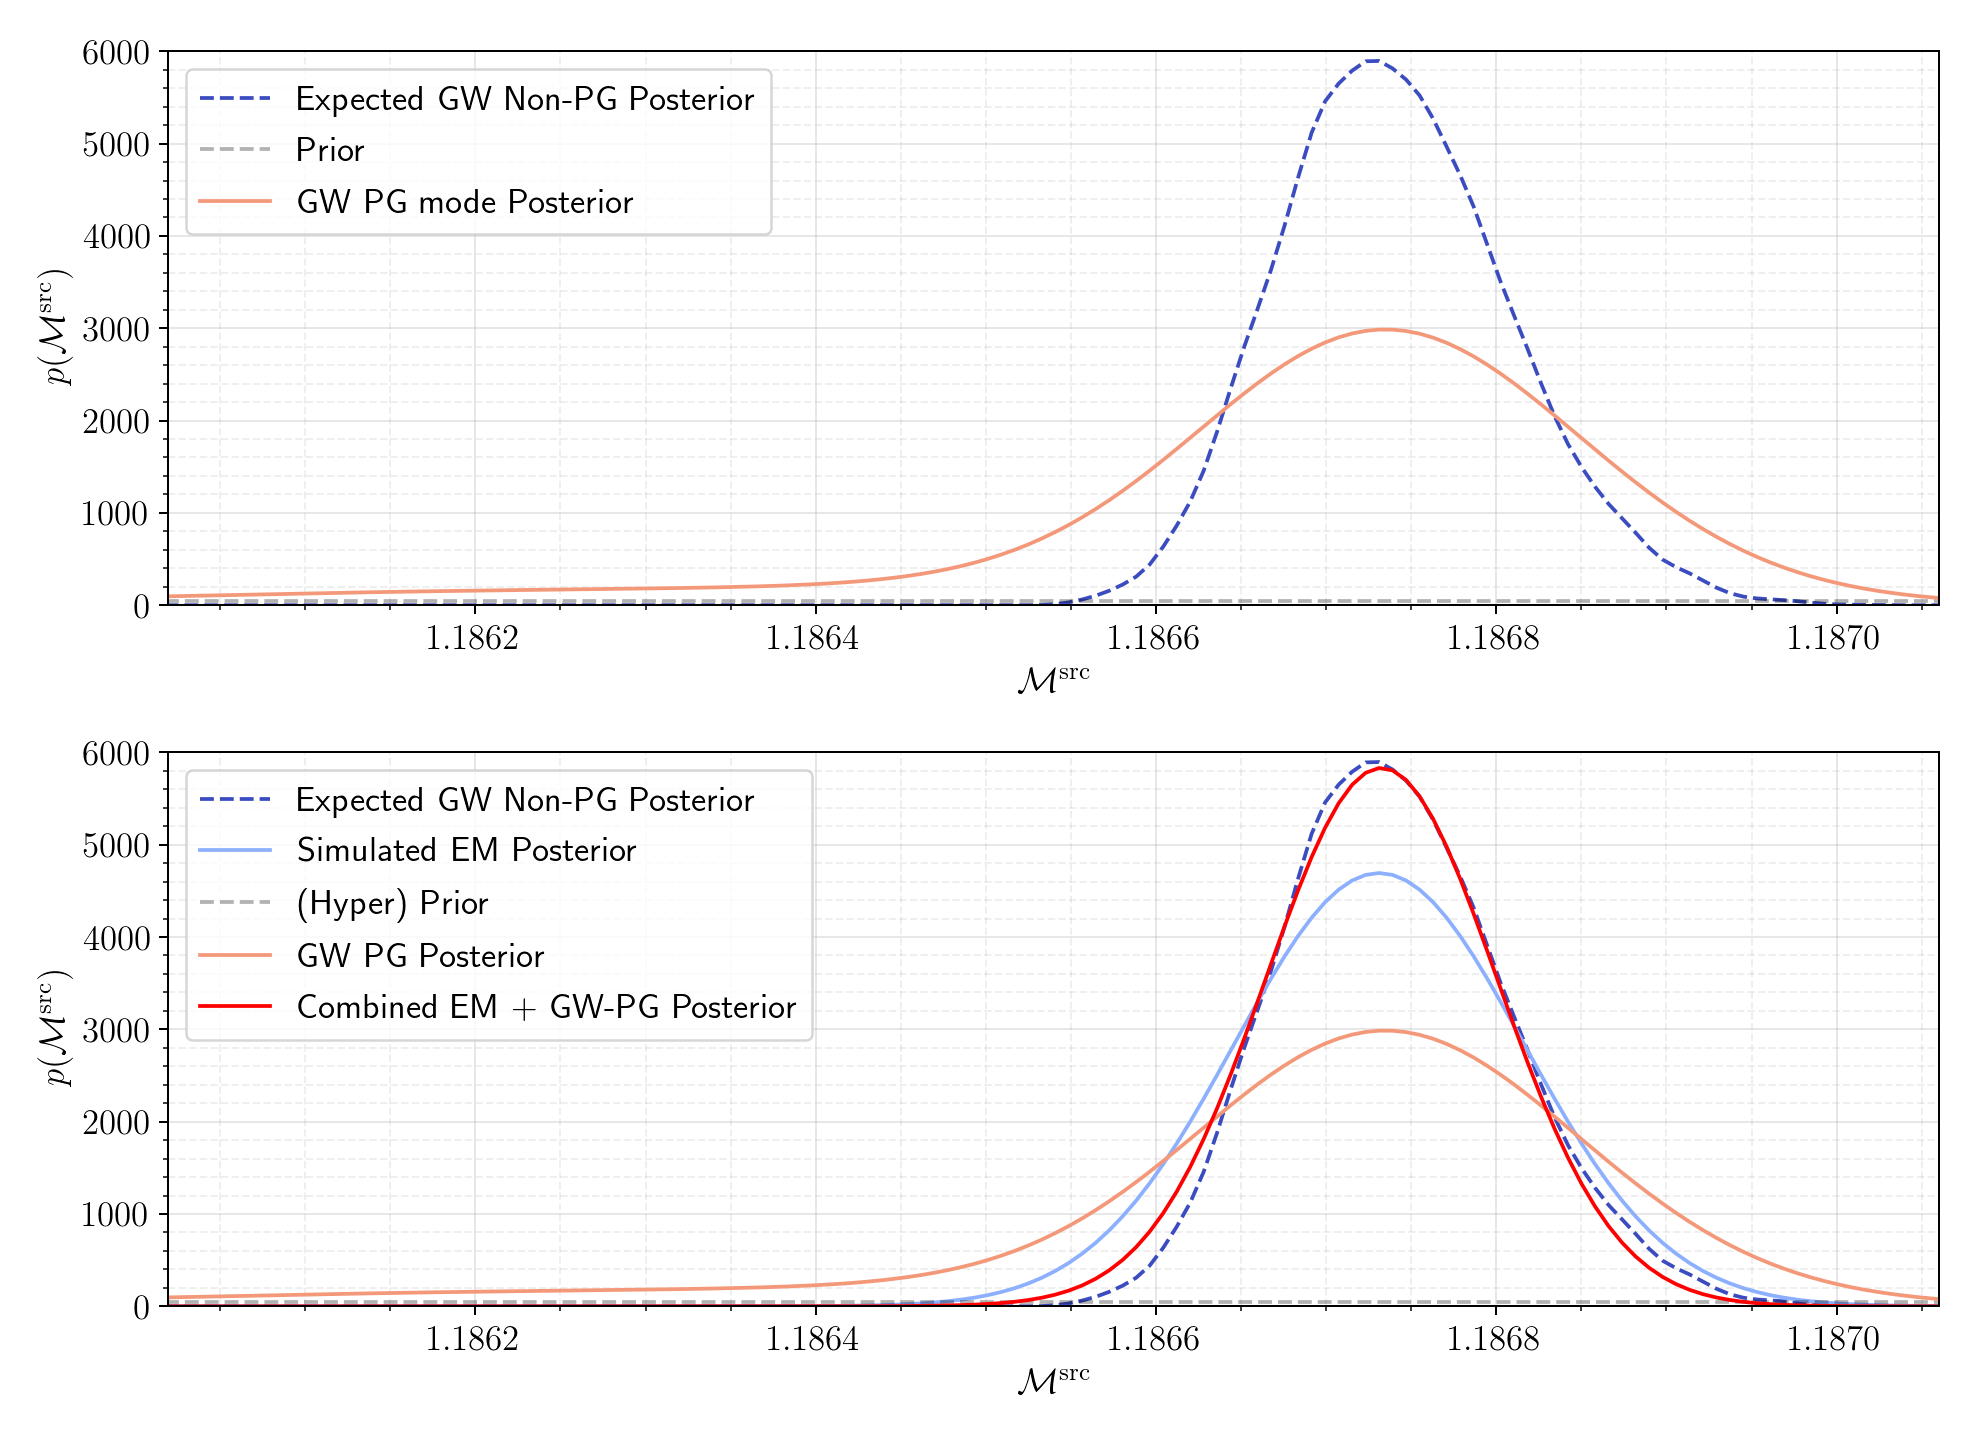
\includegraphics[width=0.9\columnwidth]{figs/chapter6/em_posterior_fix.png}
\caption{(\textit{Top}) The prior distribution on the chirp mass for two gravitational wave astrophysical hypotheses. The first hypothesis is the uniform mass and constrained equation of state constraint model from~\cite{de2018tidal}, while the second model is the $p$-$g$ mode instability hypothesis with unconstrained $\delta \phi$. The marginal posterior distributions on the chirp mass are in dashed-blue and solid, light-red, respectively. (\textit{Bottom}) Combining a simulated Gaussian electromagnetic posterior on the chirp mass (light-blue) and a prior on the chirp mass we can combine the posterior distributions from the gravitational wave data with the $p$-$g$ mode instability from the unconstrained $\delta \phi$ model with this electromagnetic posterior to construct a joint posterior distribution (solid, red) that closely matches the inferred chirp mass for GW170817 from~\cite{de2018tidal}. The simulated Gaussian electromagnetic posterior has mean centered at the maximum a posteriori value from~\cite{de2018tidal}, $\mu = 1.186731 \, M_\odot$, and standard deviation, $\sigma = 0.000085 \, M_\odot$.}
\label{fig:em_posterior_analysis}
\end{figure}

\section{Will there ever be a time when we can rule out the $p$-$g$ mode instability?}
In this section we investigate whether we can make a projection about whether future events will ever permit us to rule out the $p$-$g$ mode instability. We will have to make many assumptions in this section regarding the properties of the model, the events that we see, and the rate of mergers for binary neutron stars.

Our goal is to take advantage of the fact that Bayes factors for hypotheses are multiplicative across statistically independent events. That is to say, that with more binary neutron star events we can accumulate evidence for or against $p$-$g$ mode instability through continuous testing of these hypotheses on the individual events. The Bayes factors for $N$ events can be combined into one Bayes factor via following expression:
\begin{equation}\label{eqn:cumulative_bayes_factor}
    \mathcal{B}(\mathbf{d_1}, \mathbf{d_2}, \ldots,  \mathbf{d_{N-1}}, \mathbf{d_{N}} \, | \, \mathrm{H}_{\mathrm{NL}}, \mathrm{H}_{\mathrm{!NL}}) = \prod_{i=1}^N \mathcal{B}(\mathbf{d_i} \, | \, \mathrm{H}_{\mathrm{NL}}, \mathrm{H}_{\mathrm{!NL}}).
\end{equation}
Here the hypotheses for $p$-$g$ mode instability is denoted as $\mathrm{H}_{\mathrm{NL}}$, while the null hypothesis is denoted $\mathrm{H}_{\mathrm{!NL}}$. Note that inference with Bayes factors is equivalent to a Frequentist inference based on the likelihood rather than inference on a posterior probability. We multiply the Bayes factor by a $50 - 50$ prior odds ratio, $\left(\frac{\pi(\mathrm{H}_{\mathrm{NL}})}{\pi(\mathrm{H}_{\mathrm{!NL}})}\right)$, effectively stating no preference for either hypothesis, to convert the Bayes factor to a posterior odds ratio $\mathcal{O}$. Doing so permits us to consider the posterior odds ratio as equivalent to the Bayes factor:
\begin{equation}\label{eqn:posterior_odds_ratio}
    \mathcal{O}(\mathrm{H}_{\mathrm{NL}}, \mathrm{H}_{\mathrm{!NL}} \, | \, \mathbf{d_1}, \mathbf{d_2}, \ldots,  \mathbf{d_{N-1}}, \mathbf{d_{N}}) = \frac{\pi(\mathrm{H}_{\mathrm{NL}})}{\pi(\mathrm{H}_{\mathrm{!NL}})} \times \mathcal{B}(\mathbf{d_1}, \mathbf{d_2}, \ldots,  \mathbf{d_{N-1}}, \mathbf{d_{N}}\, | \, \mathrm{H}_{\mathrm{NL}}, \mathrm{H}_{\mathrm{!NL}}).
\end{equation}
Here $\mathcal{O}(\mathrm{H}_{\mathrm{NL}}, \mathrm{H}_{\mathrm{!NL}} \, | \, \mathbf{d_1}, \mathbf{d_2}, \ldots,  \mathbf{d_{N-1}}, \mathbf{d_{N}})$ is the posterior odds ratio, and thus setting  $\frac{\pi(\mathrm{H}_{\mathrm{NL}})}{\pi(\mathrm{H}_{\mathrm{!NL}})}$ equal to unity makes the posterior odds ratio equivalent to the Bayes factor. We will use the Bayes factor instead of the odds ratio for the duration of this section, with the understanding that they are equivalent in this scenario.

It is instructive to examine the behavior of the cumulative logarithm of the Bayes factor for the incredible case that the next several binary neutron stars are identical in signal-to-noise ratio and intrinsic properties as GW170817. Here we consider two estimators for the Bayes factor, the thermodynamic integration method which we found to have a log Bayes factor of $\mu \sim -0.38$, and at worst $\sigma \sim 0.1$, and the logspline estimator with the Savage Dickey density ratio which we found to have a log Bayes factor of $\mu \sim -0.46, \sigma \sim 0.06$. We note that the logspline estimate is not a log-normal distribution, but it this estimate is close enough to the estimates from our analysis for demonstrative purposes. The analysis of~\cite{abbott2019constraining} found a log Bayes factor of $0.03^{+0.70}_{-0.58}$ at $90 \%$ confidence using the Savage-Dickey density ratio. We model this as a Gaussian distribution in the logarithm Bayes factor with $\mu = 0.03, \sigma = 0.4$ so as to have a similar $90\%$ interval width. While for GW170817 these Bayes factor estimates are compatible, if we measure a new GW170817-like binary neutron star and measure the same Bayes factor for this new event, the cumulative Bayes factor and the uncertainty surrounding this cumulative Bayes factor propagates multiplicatively and quickly begin to exclude each other as more events are aggregated.

To illustrate this consider the case that our MCMC methods estimate the logarithm of Bayes factors for some fixed choice of prior distribution and for cumulative gravitational wave events. Consider the case that the estimator of the logarithm of the Bayes factor is a normal distribution with mean (point-estimate) $\mu$ and a standard deviation (uncertainty) $\sigma_i$:
\begin{equation}
    \widehat{\mathrm{ln} \, \mathcal{B}^{\mathrm{NL}}_{\mathrm{!NL}}}(\mathbf{d_i}) = \mathcal{N}(\mu_i, \sigma_i).
\end{equation}
Thus, the cumulative Bayes factor for many neutron star events becomes:
\begin{equation}
    \begin{array}{ll}
    \widehat{\mathrm{ln} \, \mathcal{B}^{\mathrm{NL}}_{\mathrm{!NL}}}(\mathbf{d_1}, \mathbf{d_2}, ..., \mathbf{d_N}) &\quad = \sum \limits_{i=1}^{N} \widehat{\mathrm{ln} \, \mathcal{B}^{\mathrm{NL}}_{\mathrm{!NL}}}(\mathbf{d_i}) \\ \\
    &\quad = \mathcal{N}\left(\mu = \sum \limits_{i=1}^{N} \mu_i, \, \, \sigma = \sqrt{\sum \limits_{i=1}^{N} \sigma_i^2}\right).
    \end{array}
\end{equation}
We note that if the Bayes factor point-estimate term $\mu_i$ is monotonic across events, and the uncertainty estimate from our MCMC methods $\sigma_i$ is usually consistent, then the estimator $\widehat{\mathrm{ln} \, \mathcal{B}^{\mathrm{NL}}_{\mathrm{!NL}}}(\mathbf{d_1}, ..., \mathbf{d_N})$ will tend towards a log Bayes factor that is statistically significant, for which a decision on whether nonlinear tidal effects from a $p$-$g$ mode instability is present / measurable in neutron stars.  For repetitions of the same event we see that the mean of this Gaussian distribution for the cumulative log Bayes factor grows linearly with $mu_i$, and the uncertainty grows as $\sqrt{N} \sigma_i$. However, if noise elements in the MCMC or from the data itself dilute the ability for our MCMC estimator to find a $\mu \neq 0$ or a monotonic measurement of $\mu$ then the logarithm of the Bayes factor will become overly diluted by a growing uncertainty $\sigma$.  As seen in Fig.~\ref{fig:sim_many_gw170817_divergent_bayes}, after five events, the cumulative Bayes factor estimations diverge significantly. They may be caused by different methodologies in Bayes factor estimation, by waveform systematics, by power-spectral density estimation differences, by different segments of GPS-analysis times used, the low-frequency cutoff used, or by many other possible variables that are not accounted for in this comparison. As MCMC methods for estimating Bayes factor improve this error in cumulative Bayes factor estimation should also improve.

\begin{figure}[th]
\centering
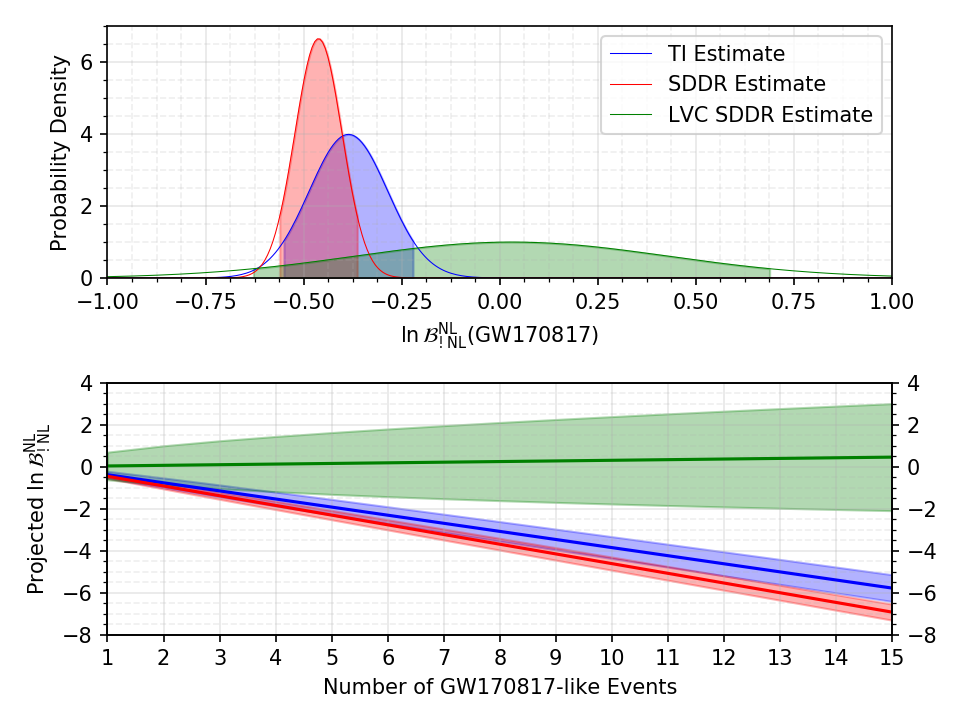
\includegraphics[width=0.9\columnwidth]{figs/chapter6/sim_many_gw170817_evidence_error_prop.png}
\caption{(\textit{Top}) A comparison of Gaussian approximations of the logarithm of the Bayes factor using different estimators or waveform systematics. Note that the LVC estimate here is a rough Gaussian approximation based on the reported bounds in~\cite{abbott2019constraining}. The $90 \%$ confidence regions are shaded in. Positive log Bayes factors are indicative of support for the $p$-$g$ mode hypothesis, while negative log Bayes factors are indicative of support for the null hypothesis. (\textit{Bottom}) For repeated GW170817-like binary neutron star mergers the cumulative logarithm of the Bayes factor for the $p$-$g$ mode hypothesis vs the null hypothesis begin to diverge in estimation. The solid lines represent the cumulative median estimates, while the shaded regions represent the cumulative $90 \%$ confidence intervals. Waveform systematics or uncontrolled variables in the Bayes factor estimation methods may be the main driver of this divergence and future meta-analyses will have to control for these sorts of uncertainty.}
\label{fig:sim_many_gw170817_divergent_bayes}
\end{figure}

A more realistic approach is to consider that the distribution of signal-to-noise ratio for binary neutron star events will not all be repeats of GW170817 but rather will follow some other distribution. To do so explore this we need to model the expected signal-to-noise-ratio, $\rho$, of events that we expect to see with gravitational wave observatories. Fortunately, this work has already been done in~\cite{schutz2011networks, chen2014loudest}. We can expect that for a network of interferometers with a signal to noise ratio detection threshold of $\rho_{\mathrm{threshold}}$ that our distribution will follow the rule:
\begin{equation}\label{eqn:universal_snr}
    p(\rho) = 3 \, \frac{\rho_{\mathrm{threshold}}^3}{\rho^4}.
\end{equation}
This expression is a normalized probability distribution function in so far as we only permit $\rho > \rho_{\mathrm{threshold}}$ and let $\rho$ go to positive infinity. Given this probability distribution we can expect our average $\rho$ to be equal to $\frac{3}{2} \rho_{\mathrm{threshold}}$. If we assume a very conservative $\rho_{\mathrm{threshold}} = 11$, then the probability of attaining gravitational wave neutron star mergers as loud as or louder than GW170817 ($\rho \approx 34$) is slightly higher than $3~\%$. At a signal-to-noise ratio of $\sim 34$ we have found that the $p$-$g$ mode instability hypothesis has a Bayes factor of approximately $1$, and we expect that $97 \%$ of neutron star detections will be quieter than GW170817 for which the Bayes factor will in all likelihood be unity as well due to parameter degeneracies. Thus we see that in the long-term we may have to wait for hundreds of binary neutron star mergers to be able to make a decision on the validity of the $p$-$g$ mode instability hypothesis, for-or-against. Biases and difficulties in the MCMC method for hypothesis testing, the noise in the detector, and waveform systematics in all likelihood will make this endeavor all the more difficult.

And so to answer the question of the subsection, ``Will there ever be a time when we can rule out $p$-$g$ mode instability?", depends on a number of factors. Firstly, what do we mean when we say the $p$-$g$ mode instability, e.g., which priors, which waveform model, with which MCMC method, and under which assumptions? We have ruled out some sorts of $p$-$g$ mode instability in this paper and the marginal posterior densities from~\cite{abbott2019constraining} similarly tell us that some $p$-$g$ mode parameters are not favored by the data.  and (b) whether the theory has yielded any new or interesting observations or features of the data that cannot be explained by another model. In all likelihood the theory will dissolve into obscurity, much as it currently stands today. While the $p$-$g$ mode hypothesis is perhaps not very interesting in its own right, it shows the ambiguities and difficulties inherent in Bayesian gravitational wave astrophysical analysis. We hope that our exploration and explanation of the problem prompts greater thoughtfulness with respect to statistical analysis and experimental design.
